\documentclass[12pt,a4paper,oneside]{book}

% ==============================================================================
% preamble.tex - הגדרות חבילות, עברית מלאה RTL, גופנים, כותרות ספר, טבלאות וגרפים
% מותאם לקומפילציה מהירה ב-LuaLaTeX לפי כללי "מהבעיה אל ה-PDF" ושיעור L03 (ד"ר יורם סגל)
% ==============================================================================

\usepackage{geometry}
\geometry{
  a4paper,
  top=2.5cm,
  bottom=2.5cm,
  inner=3.0cm,   % 2.5cm + 0.5cm Gutter (שוליים + תוספת כריכה לפי טבלה 11.1)
  outer=2.5cm,
  headheight=16pt
}

% מתמטיקה ונוסחאות
\usepackage{amsmath,amssymb,amsfonts}

% כיווניות ושפות ב-LuaLaTeX באמצעות babel + bidi=basic (תקן L03 ופרק 12)
\makeatletter\@namedef{ver@luatexbase.sty}{2015/10/04 v1.3}\makeatother
\usepackage[bidi=basic,provide=*,shorthands=off]{babel}
\babelprovide[import,main]{hebrew}
\babelprovide[import]{english}
\usepackage{fontspec}

% הגדרת גופנים תקניים מתוך מערכת ההפעלה Windows (לפי טבלה 11.1 וטבלה 12.1)
\babelfont{rm}[
  Path=C:/Windows/Fonts/,
  UprightFont=times.ttf,
  BoldFont=timesbd.ttf,
  ItalicFont=timesi.ttf,
  BoldItalicFont=timesbi.ttf
]{Times New Roman}

\babelfont[hebrew]{rm}[
  Script=Hebrew,
  Path=C:/Windows/Fonts/,
  UprightFont=david.ttf,
  BoldFont=davidbd.ttf,
  ItalicFont=david.ttf,
  BoldItalicFont=davidbd.ttf
]{David}

\babelfont{sf}[
  Path=C:/Windows/Fonts/,
  UprightFont=arial.ttf,
  BoldFont=arialbd.ttf,
  ItalicFont=ariali.ttf,
  BoldItalicFont=arialbi.ttf
]{Arial}

\babelfont[hebrew]{sf}[
  Script=Hebrew,
  Path=C:/Windows/Fonts/,
  UprightFont=arial.ttf,
  BoldFont=arialbd.ttf,
  ItalicFont=ariali.ttf,
  BoldItalicFont=arialbi.ttf
]{Arial}

\babelfont{tt}[
  Path=C:/Windows/Fonts/,
  UprightFont=cour.ttf,
  BoldFont=courbd.ttf
]{Courier New}

\babelfont[hebrew]{tt}[
  Script=Hebrew,
  Path=C:/Windows/Fonts/,
  UprightFont=cour.ttf,
  BoldFont=courbd.ttf
]{Courier New}

\newcommand{\hebrewfont}{\rmfamily}
\newcommand{\hebrewfontsf}{\sffamily}
\newcommand{\hebrewfonttt}{\ttfamily}
\newcommand{\englishfont}{\rmfamily}
\newcommand{\englishfontsf}{\sffamily}
\newcommand{\englishfonttt}{\ttfamily}

% תאימות מלאה לפקודות polyglossia/babel עבור טקסט דו-כיווני (BiDi) - בטוח גם במצב מתמטיקה
\providecommand{\texthebrew}[1]{\ifmmode\mbox{\foreignlanguage{hebrew}{#1}}\else\foreignlanguage{hebrew}{#1}\fi}
\providecommand{\textenglish}[1]{\ifmmode\mathrm{#1}\else\foreignlanguage{english}{#1}\fi}
\newenvironment{hebrew}{\begin{otherlanguage}{hebrew}}{\end{otherlanguage}}
\newenvironment{english}{\begin{otherlanguage}{english}}{\end{otherlanguage}}

% ריווח שורות 1.5 ומניעת כותרות יתומות (טבלה 11.1 ופרק 19.4)
\linespread{1.28}\selectfont
\newcommand{\onehalfspacing}{\linespread{1.28}\selectfont}
\newcommand{\needspace}[1]{\par\nopagebreak\vspace{0pt}}

% תמיכה בפרמטרים אופציונליים ברשימות enumerate ו-itemize
\let\origenumerate\enumerate
\let\endorigenumerate\endenumerate
\renewenvironment{enumerate}[1][]{\origenumerate}{\endorigenumerate}
\let\origitemize\itemize
\let\endorigitemize\enditemize
\renewenvironment{itemize}[1][]{\origitemize}{\endorigitemize}

% צבעים ארגוניים עקביים לכל המסמך (פרק 15 ופרק 16.6)
\usepackage{xcolor}
\definecolor{BrandNavy}{RGB}{18, 48, 89}
\definecolor{BrandBlue}{RGB}{32, 92, 168}
\definecolor{BrandLightBlue}{RGB}{235, 243, 252}
\definecolor{BrandTeal}{RGB}{16, 112, 104}
\definecolor{BrandLightTeal}{RGB}{234, 247, 245}
\definecolor{BrandGold}{RGB}{184, 115, 20}
\definecolor{BrandLightGold}{RGB}{253, 247, 234}
\definecolor{BrandRed}{RGB}{178, 34, 45}
\definecolor{BrandLightRed}{RGB}{253, 237, 238}
\definecolor{BrandGray}{RGB}{244, 246, 249}
\definecolor{TableHeaderBg}{RGB}{218, 229, 244}

% גרפיקה, איורים, TikZ ו-pgfplots (פרק 16)
\usepackage{graphicx}
\graphicspath{{figures/}}
\usepackage{tikz}
\usetikzlibrary{arrows.meta,positioning,shapes.geometric,calc,patterns,backgrounds,fit,babel}
\usepackage{pgfplots}
\pgfplotsset{compat=1.18}

% טבלאות מעוצבות (פרק 11 ופרק 16.5)
\usepackage{array}
\usepackage{tabularx}
\newcommand{\toprule}{\noalign{\hrule height 1.1pt\vspace{3pt}}}
\newcommand{\midrule}{\noalign{\vspace{2pt}\hrule height 0.6pt\vspace{3pt}}}
\newcommand{\bottomrule}{\noalign{\vspace{2pt}\hrule height 1.1pt}}
\newcommand{\addlinespace}[1][4pt]{}
\newcommand{\rowcolors}[3]{}
\newcommand{\rowcolor}[1]{}
\newcolumntype{R}[1]{>{\raggedleft\arraybackslash}p{#1}}
\newcolumntype{L}[1]{>{\raggedright\arraybackslash}p{#1}}
\newcolumntype{C}[1]{>{\centering\arraybackslash}p{#1}}
\newcolumntype{Y}{>{\raggedleft\arraybackslash}X}

% הגנה מלאה על מספור פרקים, סעיפים, איורים, טבלאות ומשוואות מפני היפוך BiDi (טבלה 14.3 וטבלה 15.5)
\setcounter{secnumdepth}{3}
\setcounter{tocdepth}{3}
\renewcommand{\thechapter}{\textenglish{\arabic{chapter}}}
\renewcommand{\thesection}{\textenglish{\arabic{chapter}.\arabic{section}}}
\renewcommand{\thesubsection}{\textenglish{\arabic{chapter}.\arabic{section}.\arabic{subsection}}}
\renewcommand{\thesubsubsection}{\textenglish{\arabic{chapter}.\arabic{section}.\arabic{subsection}.\arabic{subsubsection}}}
\renewcommand{\thefigure}{\textenglish{\arabic{chapter}.\arabic{figure}}}
\renewcommand{\thetable}{\textenglish{\arabic{chapter}.\arabic{table}}}
\renewcommand{\theequation}{\arabic{chapter}.\arabic{equation}}

% עיצוב כותרות פרקים וסעיפים וכותרות רצות (ללא תלות בחבילות חיצוניות)
\makeatletter
\def\@makechapterhead#1{%
  \vspace*{10\p@}%
  {\parindent \z@ \raggedleft \normalfont\sffamily
    \ifnum \c@secnumdepth >\m@ne
      \Large\bfseries\color{BrandBlue} \@chapapp\space \thechapter
      \par\nobreak
      \vskip 6\p@
    \fi
    \interlinepenalty\@M
    {\color{BrandNavy}\hrule height 1.5pt}\vskip 8\p@
    \Huge \bfseries \color{BrandNavy} #1\par\nobreak
    \vskip 8\p@
    {\color{BrandNavy}\hrule height 0.8pt}
    \vskip 22\p@
  }}
\def\@makeschapterhead#1{%
  \vspace*{10\p@}%
  {\parindent \z@ \raggedleft \normalfont\sffamily
    \interlinepenalty\@M
    {\color{BrandNavy}\hrule height 1.5pt}\vskip 8\p@
    \Huge \bfseries \color{BrandNavy} #1\par\nobreak
    \vskip 8\p@
    {\color{BrandNavy}\hrule height 0.8pt}
    \vskip 22\p@
  }}
\renewcommand\section{\@startsection {section}{1}{\z@}%
  {-3.2ex \@plus -1ex \@minus -.2ex}%
  {1.8ex \@plus.2ex}%
  {\normalfont\sffamily\Large\bfseries\color{BrandNavy}}}
\renewcommand\subsection{\@startsection{subsection}{2}{\z@}%
  {-2.8ex\@plus -1ex \@minus -.2ex}%
  {1.2ex \@plus .2ex}%
  {\normalfont\sffamily\large\bfseries\color{BrandBlue}}}
\renewcommand\subsubsection{\@startsection{subsubsection}{3}{\z@}%
  {-2.2ex\@plus -1ex \@minus -.2ex}%
  {0.8ex \@plus .2ex}%
  {\normalfont\sffamily\normalsize\bfseries\color{BrandTeal}}}

% כותרות עליונות ותחתונות עם כיוון מפורש בכל משבצת (טבלה 14.3 ופרק 15.10)
\def\ps@fancy{%
  \def\@oddhead{\vbox to \headheight{\hbox to \textwidth{\footnotesize\color{BrandNavy}\texthebrew{דוח מכין לפרויקט מחקר: מבצעי המימון בנדל"ן וקיר המסירות }\textenglish{2026--2027}\hfill\color{BrandBlue}\texthebrew{סמינריון מחקרי בניהול טכנולוגיות ומימון}}\vss\hrule height 0.5pt}}%
  \def\@evenhead{\@oddhead}%
  \def\@oddfoot{\vbox{\hrule height 0.4pt\vskip 3pt\hbox to \textwidth{\footnotesize\color{BrandNavy}\textenglish{\copyright\ 2026}\ \texthebrew{כל הזכויות שמורות לצוות המחקר}\hfill\texthebrew{עמוד }\textenglish{\thepage}}}}%
  \def\@evenfoot{\@oddfoot}%
}
\def\ps@plain{%
  \def\@oddhead{}%
  \def\@evenhead{}%
  \def\@oddfoot{\vbox{\hrule height 0.4pt\vskip 3pt\hbox to \textwidth{\footnotesize\color{BrandNavy}\textenglish{\copyright\ 2026}\ \texthebrew{כל הזכויות שמורות לצוות המחקר}\hfill\texthebrew{עמוד }\textenglish{\thepage}}}}%
  \def\@evenfoot{\@oddfoot}%
}
\makeatother
\pagestyle{fancy}

% תיבות מעוצבות (tcolorbox) - מסגרת ב-LTR ותוכן ב-RTL לפי כלל 6 בפרומפט B1 (פרק 14.7)
\usepackage{tcolorbox}

% 1. תיבת "למה זה חשוב למנהל / לקובע המדיניות"
\newenvironment{managerbox}[1][למה זה חשוב למנהל ולקובע המדיניות]{%
  \par\medskip%
  \begin{english}%
  \begin{tcolorbox}[
    colback=BrandLightGold,
    colframe=BrandGold,
    colbacktitle=BrandGold,
    coltitle=white,
    boxrule=1pt,
    arc=3pt,
    left=10pt,right=10pt,top=8pt,bottom=8pt,
    title={\hfill\textbf{\sffamily\texthebrew{#1}}}
  ]%
  \begin{hebrew}%
}{%
  \end{hebrew}%
  \end{tcolorbox}%
  \end{english}%
  \par\medskip%
}

% 2. תיבת הגדרה / מודל מתמטי / מסר מרכזי
\newenvironment{modelbox}[1][הגדרה ומודל אנליטי]{%
  \par\medskip%
  \begin{english}%
  \begin{tcolorbox}[
    colback=BrandLightBlue,
    colframe=BrandNavy,
    colbacktitle=BrandNavy,
    coltitle=white,
    boxrule=1pt,
    arc=3pt,
    left=10pt,right=10pt,top=8pt,bottom=8pt,
    title={\hfill\textbf{\sffamily\texthebrew{#1}}}
  ]%
  \begin{hebrew}%
}{%
  \end{hebrew}%
  \end{tcolorbox}%
  \end{english}%
  \par\medskip%
}

% 3. תיבת מלכודת מתודולוגית / אזהרת סיכון
\newenvironment{warningbox}[1][מלכודת מתודולוגית ומוקד סיכון]{%
  \par\medskip%
  \begin{english}%
  \begin{tcolorbox}[
    colback=BrandLightRed,
    colframe=BrandRed,
    colbacktitle=BrandRed,
    coltitle=white,
    boxrule=1pt,
    arc=3pt,
    left=10pt,right=10pt,top=8pt,bottom=8pt,
    title={\hfill\textbf{\sffamily\texthebrew{#1}}}
  ]%
  \begin{hebrew}%
}{%
  \end{hebrew}%
  \end{tcolorbox}%
  \end{english}%
  \par\medskip%
}

% 4. תיבת יישום בפרויקט המחקר ("בפרויקט שלנו")
\newenvironment{projectbox}[1][יישום בפרויקט המחקר שלנו]{%
  \par\medskip%
  \begin{english}%
  \begin{tcolorbox}[
    colback=BrandLightTeal,
    colframe=BrandTeal,
    colbacktitle=BrandTeal,
    coltitle=white,
    boxrule=1pt,
    arc=3pt,
    left=10pt,right=10pt,top=8pt,bottom=8pt,
    title={\hfill\textbf{\sffamily\texthebrew{#1}}}
  ]%
  \begin{hebrew}%
}{%
  \end{hebrew}%
  \end{tcolorbox}%
  \end{english}%
  \par\medskip%
}

% פקודות עזר דו-כיווניות (BiDi) לפי Prompt B1 (פרק 14.7) - בטוחות במצב טקסט ובמצב מתמטיקה
\newcommand{\en}[1]{\ifmmode\mathrm{#1}\else\foreignlanguage{english}{#1}\fi}
\newcommand{\num}[1]{\ifmmode#1\else\foreignlanguage{english}{#1}\fi}
\newcommand{\pct}[1]{\ifmmode#1\%\else\foreignlanguage{english}{#1\%}\fi}
\newcommand{\nis}[1]{\ifmmode#1\;\mbox{\foreignlanguage{hebrew}{ש"ח}}\else\foreignlanguage{english}{#1}\ \foreignlanguage{hebrew}{ש"ח}\fi}
\newcommand{\usd}[1]{\ifmmode\$#1\else\foreignlanguage{english}{\$#1}\fi}
\newcommand{\hebmath}[1]{\mbox{\foreignlanguage{hebrew}{#1}}}

% הדפסת ביבליוגרפיה בתקן IEEE מתוך קובץ references.bib המסונכרן ל-resources/bibliography_items.tex
\newcommand{\printbibliography}{%
  \chapter{רשימת מקורות וביבליוגרפיה (\en{References})}%
  \IfFileExists{resources/bibliography_items.tex}{% Auto-generated IEEE bibliography items from references.bib
\begin{english}
\begin{thebibliography}{99}
\small
\bibitem{segal2026prep} \textbf{Segal, Yoram}, ``From Problem to PDF: The Professional Preparatory Report (מהבעיה אל ה-PDF: המדריך לדוח המכין המקצועי),'' \textit{Bar-Ilan University, Department of Management}, 2026.
\bibitem{ulrich2020product} \textbf{Ulrich, Karl T. and Eppinger, Steven D. and Yang, Maria C.}, ``Product Design and Development,'' \textit{McGraw-Hill Education}, 2020.
\bibitem{boi2024annual} \textbf{Bank of Israel}, ``Bank of Israel Annual Report for 2024 -- Chapter 9: The Housing Market and Construction Sector,'' \textit{Bank of Israel Research Department}, 2025.
\bibitem{boi2025stability} \textbf{Bank of Israel}, ``Financial Stability Report -- First Half of 2025: Credit Risks in Real Estate and Developer Promotions,'' \textit{Bank of Israel Financial Stability Division}, 2025.
\bibitem{mof2025economist} \textbf{Chief Economist Department}, ``Real Estate Market Review: Analysis of Contractor Cash-Flow Promotions (20/80) and Investor Purchases,'' \textit{Israel Ministry of Finance}, 2025.
\bibitem{cbs2026dwellings} \textbf{Central Bureau of Statistics (CBS)}, ``New Dwellings Sold and Unsold Inventory in Israel: Statistical Bulletin Q1--Q3 2026,'' \textit{Israel Central Bureau of Statistics}, 2026.
\bibitem{boi2025directive} \textbf{Banking Supervision Department}, ``Temporary Order Amending Proper Conduct of Banking Business Directives 329 and 311: Restrictions on Bullet/Balloon Housing Loans and Project Accompaniment Risk Weights (March 2025),'' \textit{Bank of Israel}, 2025.
\bibitem{mian2009consequences} \textbf{Mian, Atif and Sufi, Amir}, ``The Consequences of Mortgage Credit Expansion: Evidence from the U.S. Mortgage Default Crisis,'' \textit{The Quarterly Journal of Economics}, vol.~124, no.~4, pp.~1449--1496, 2009. DOI: \texttt{10.1162/qjec.2009.124.4.1449}.
\bibitem{mayer2009rise} \textbf{Mayer, Christopher and Pence, Karen and Sherlund, Shane M.}, ``The Rise in Mortgage Defaults,'' \textit{Journal of Economic Perspectives}, vol.~23, no.~1, pp.~27--50, 2009. DOI: \texttt{10.1257/jep.23.1.27}.
\bibitem{segal2026l03} \textbf{Segal, Yoram}, ``L03: Create PDF Documents with LaTeX Vibe Coding (שיעור 3: מסמך PDF מקצועי בלטך),'' \textit{University of Haifa, Course Lecture Notes}, 2026.
\bibitem{doran1981smart} \textbf{Doran, George T.}, ``There's a S.M.A.R.T. Way to Write Management's Goals and Objectives,'' \textit{Management Review}, vol.~70, no.~11, pp.~35--36, 1981.
\bibitem{ita2025carman} \textbf{Israel Tax Authority}, ``CARMAN Real Estate Transactions Database : Methodological Documentation and Reporting Standards,'' \textit{Ministry of Finance, Jerusalem}, 2025.
\bibitem{webster2002analyzing} \textbf{Webster, Jane and Watson, Richard T.}, ``Analyzing the Past to Prepare for the Future: Writing a Literature Review,'' \textit{MIS Quarterly}, vol.~26, no.~2, pp.~xiii--xxiii, 2002.
\bibitem{stiglitz1981credit} \textbf{Stiglitz, Joseph E. and Weiss, Andrew}, ``Credit Rationing in Markets with Imperfect Information,'' \textit{The American Economic Review}, vol.~71, no.~3, pp.~393--410, 1981.
\bibitem{jensen1976theory} \textbf{Jensen, Michael C. and Meckling, William H.}, ``Theory of the Firm: Managerial Behavior, Agency Costs and Ownership Structure,'' \textit{Journal of Financial Economics}, vol.~3, no.~4, pp.~305--360, 1976. DOI: \texttt{10.1016/0304-405X(76)90026-X}.
\bibitem{minsky1992financial} \textbf{Minsky, Hyman P.}, ``The Financial Instability Hypothesis,'' \textit{The Jerome Levy Economics Institute Working Paper}, no.~74, pp.~1--10, 1992.
\bibitem{kindleberger2011manias} \textbf{Kindleberger, Charles P. and Aliber, Robert Z.}, ``Manias, Panics, and Crashes: A History of Financial Crises,'' \textit{Palgrave Macmillan}, 2011.
\bibitem{reinhart2009this} \textbf{Reinhart, Carmen M. and Rogoff, Kenneth S.}, ``This Time Is Different: Eight Centuries of Financial Folly,'' \textit{Princeton University Press}, 2009.
\bibitem{keys2010did} \textbf{Keys, Benjamin J. and Mukherjee, Tanmoy and Seru, Amit and Vig, Vikrant}, ``Did Securitization Lead to Lax Screening? Evidence from Subprime Loans,'' \textit{The Quarterly Journal of Economics}, vol.~125, no.~1, pp.~307--362, 2010. DOI: \texttt{10.1162/qjec.2010.125.1.307}.
\bibitem{gorton2009securitized} \textbf{Gorton, Gary B.}, ``Slapped in the Face by the Invisible Hand: Banking and the Panic of 2007,'' \textit{Federal Reserve Bank of Atlanta Financial Markets Conference}, pp.~1--43, 2009.
\bibitem{ben2011inflated} \textbf{Ben-David, Itzhak}, ``Financial Constraints and Inflated Home Prices during the Real Estate Boom,'' \textit{American Economic Journal: Applied Economics}, vol.~3, no.~3, pp.~55--87, 2011. DOI: \texttt{10.1257/app.3.3.55}.
\bibitem{ghent2011recourse} \textbf{Ghent, Andra C. and Kudlyak, Marianna}, ``Recourse and Residential Mortgage Default: Evidence from US States,'' \textit{The Review of Financial Studies}, vol.~24, no.~9, pp.~3139--3186, 2011. DOI: \texttt{10.1093/rfs/hhr055}.
\bibitem{salelaw1974} \textbf{Knesset of Israel}, ``Sale (Apartments) (Assurance of Investments of Persons Acquiring Apartments) Law, 5735-1974 (חוק המכר  , התשל"ה-1974),'' \textit{Book of Laws (Sefer HaChukim)}, 1974.
\bibitem{sandberg2011ways} \textbf{Sandberg, J\"orgen and Alvesson, Mats}, ``Ways of Constructing Research Questions: Gap-Spotting or Problematization?,'' \textit{Organization}, vol.~18, no.~1, pp.~23--44, 2011.
\bibitem{bernanke2010monetary} \textbf{Bernanke, Ben S.}, ``Monetary Policy and the Housing Bubble,'' \textit{Speech at the Annual Meeting of the American Economic Association}, pp.~1--22, 2010.
\bibitem{foote2008subprime} \textbf{Foote, Christopher L. and Gerardi, Kristopher and Goette, Lorenz and Willen, Paul S.}, ``Subprime Facts: What (We Think) We Know about the Subprime Crisis and What We Don't,'' \textit{Federal Reserve Bank of Boston Public Policy Discussion Papers}, no.~08-2, pp.~1--64, 2008.
\bibitem{pugh1991total} \textbf{Pugh, Stuart}, ``Total Design: Integrated Methods for Successful Product Engineering,'' \textit{Addison-Wesley}, 1991.
\bibitem{pmbok2021} \textbf{Project Management Institute}, ``A Guide to the Project Management Body of Knowledge (PMBOK Guide),'' \textit{Project Management Institute}, 2021.
\bibitem{iso31000} \textbf{International Organization for Standardization}, ``ISO 31000:2018 -- Risk Management -- Guidelines,'' \textit{ISO}, 2018.
\end{thebibliography}
\end{english}}{\input{bibliography_items.tex}}%
}

% קישורים פנימיים וחיצוניים (hyperref נטען אחרון)
\usepackage[unicode]{hyperref}
\hypersetup{
  colorlinks=true,
  linkcolor=BrandNavy,
  citecolor=BrandBlue,
  urlcolor=BrandTeal,
  pdftitle={דוח מכין לפרויקט מחקר: מבצעי המימון הקבלניים וקיר המסירות 2026-2027},
  pdfauthor={צוות המחקר בהנחיית מתודולוגיית ד"ר יורם סגל}
}


\begin{document}

% ==============================================================================
% החלקים המקדמיים (Frontmatter) - ממוספרים בספרות רומיות קטנות (פרק 2 ופרק 12)
% ==============================================================================
\frontmatter

% ------------------------------------------------------------------------------
% 1. דף השער (ללא מספר עמוד וללא מילות מפתח - סעיפים 2.1 ו-12.2 בספר של ד"ר סגל)
% ------------------------------------------------------------------------------
\begin{titlepage}
\thispagestyle{empty}
\begin{english}
\begin{tikzpicture}[remember picture, overlay]
  % מסגרת כפולה ממלכתית סביב עמוד השער (איור 12.2)
  \draw[line width=2.2pt, color=BrandNavy]
    ($(current page.north west) + (1.2cm,-1.2cm)$)
    rectangle
    ($(current page.south east) + (-1.2cm,1.2cm)$);
  \draw[line width=0.8pt, color=BrandBlue]
    ($(current page.north west) + (1.42cm,-1.42cm)$)
    rectangle
    ($(current page.south east) + (-1.42cm,1.42cm)$);
\end{tikzpicture}
\end{english}

\begin{center}
  \vspace*{0.2cm}
  {\hebrewfontsf\large\bfseries\color{BrandNavy}
  אוניברסיטת חיפה / אוניברסיטת בר-אילן --- הפקולטה לניהול וכלכלה\\
  המחלקה לניהול טכנולוגיות ומימון --- סמינריון מחקרי (\en{5523001})\\[0.5cm]}

  % איור שער וקטורי בסגנון חוברות הקורס (איור 12.2)
  \begin{english}
  \begin{tikzpicture}[scale=0.92, transform shape]
    \fill[BrandNavy] (0,0) rectangle (11.6,4.2);
    \fill[BrandBlue!85!black] (0.2,0.2) rectangle (11.4,4.0);
    \node[anchor=north, text=white, font=\Large\bfseries] at (5.8,3.75)
      {\texthebrew{מהבעיה המאקרו-מימונית אל סימולציית העמידות}};

    % כרטיסייה 1: שוק הדיור 2022-2026
    \fill[white, rounded corners=4pt] (0.7,0.55) rectangle (3.8,2.85);
    \fill[BrandGold] (0.7,2.45) rectangle (3.8,2.85);
    \node[text=white, font=\small\bfseries] at (2.25,2.65) {\texthebrew{מבצעי קבלן }\en{20/80}};
    \node[text=BrandNavy, font=\small\bfseries] at (2.25,1.85) {\en{>85,000}\ \texthebrew{דירות}};
    \node[text=BrandRed, font=\footnotesize\bfseries] at (2.25,1.25) {\texthebrew{הנחת }\en{NPV}\ \texthebrew{סמויה}};
    \node[text=gray!80!black, font=\scriptsize] at (2.25,0.80) {\en{2022--2026}};

    % כרטיסייה 2: המנוע האנליטי
    \fill[white, rounded corners=4pt] (4.25,0.55) rectangle (7.35,2.85);
    \fill[BrandTeal] (4.25,2.45) rectangle (7.35,2.85);
    \node[text=white, font=\small\bfseries] at (5.8,2.65) {\texthebrew{מודל }\en{Monte Carlo}};
    \node[text=BrandNavy, font=\small\bfseries] at (5.8,1.85) {\en{Payment Shock}};
    \node[text=BrandTeal, font=\footnotesize\bfseries] at (5.8,1.25) {\en{Stress Test (DSCR)}};
    \node[text=gray!80!black, font=\scriptsize] at (5.8,0.80) {\en{Python + LaTeX}};

    % כרטיסייה 3: קיר המסירות 2026-2027
    \fill[white, rounded corners=4pt] (7.8,0.55) rectangle (10.9,2.85);
    \fill[BrandRed] (7.8,2.45) rectangle (10.9,2.85);
    \node[text=white, font=\small\bfseries] at (9.35,2.65) {\texthebrew{קיר המסירות}};
    \node[text=BrandNavy, font=\small\bfseries] at (9.35,1.85) {\en{2026--2027}};
    \node[text=BrandBlue, font=\footnotesize\bfseries] at (9.35,1.25) {\texthebrew{יציבות }\en{CET1}\ \texthebrew{ויזמים}};
    \node[text=gray!80!black, font=\scriptsize] at (9.35,0.80) {\texthebrew{מול ארה"ב }\en{2008}};
  \end{tikzpicture}
  \end{english}

  \vspace{0.55cm}

  {\hebrewfontsf\LARGE\bfseries\color{BrandNavy}
  מבצעי המימון הקבלניים, הלוואות הבלון ומינוף היזמים בשוק הדיור הישראלי (\num{2022--2026}) בראי משבר הסאב-פריים האמריקאי (\num{2008})\\[0.25cm]}

  {\hebrewfontsf\Large\bfseries\color{BrandBlue}
  ניתוח השוואתי ומודל סימולציה לבחינת עמידות המערכת הבנקאית והיזמית לקראת "קיר המסירות" (\num{2026--2027})\\[0.35cm]}

  \begin{english}
  {\large\bfseries\color{BrandNavy}
  Developer Financing Promotions, Balloon Loans, and Developer Leverage in the Israeli Housing Market (2022--2026) vs.\ the 2008 U.S.\ Subprime Crisis:\\[0.12cm]
  \normalsize\bfseries\color{BrandBlue}
  A Comparative Analysis and Stress-Testing Framework for the 2026--2027 ``Delivery Wall''}
  \end{english}

  \vspace{0.45cm}
  {\hebrewfontsf\large\bfseries\color{BrandTeal}
  דוח מכין לפרויקט מחקר (\en{Preliminary Research \& Design Report})\\[0.4cm]}

  {\normalsize
  \textbf{מוגש על ידי צוות המחקר:} יחידת המחקר למימון נדל"ן ויציבות פיננסית\\
  \textbf{מנחה מתודולוגי ואקדמי:} על פי מתווה "מהבעיה אל ה-\en{PDF}" מאת ד"ר יורם סגל (\en{Dr.\ Yoram Segal})\\
  \textbf{מוסד שותף למחקר:} מעבדת סימולציות סיכוני אשראי ומאקרו-יציבות\\[0.35cm]
  \textbf{תאריך הגשה:} \num{15-11-2026} (\texthebrew{סמסטר א', שנת הלימודים תשפ"ז})\\[0.35cm]}

  {\small\color{BrandNavy}
  כל הזכויות שמורות לצוות המחקר ולד"ר יורם סגל \en{\copyright\ 2026}\\
  \en{\copyright\ 2026 All Rights Reserved --- Research Team \& Dr.\ Yoram Segal.}}
\end{center}
\end{titlepage}

% ------------------------------------------------------------------------------
% 2. עמוד זכויות ושיוך אקדמי (עמוד ii)
% ------------------------------------------------------------------------------
\newpage
\vspace*{\fill}
\begin{center}
  \textbf{דוח מכין לפרויקט מחקר כלכלי-מימוני השוואתי (\en{Preliminary Research Report})}\\[0.3cm]
  נכתב, עומד וקומפל ב-\en{LuaLaTeX} בהתאם לכללי המבנה, הכיווניות (\en{BiDi}) ובקרת האיכות\\
  מתוך הספר \textbf{"מהבעיה אל ה-\en{PDF}: המדריך לדוח המכין המקצועי"} וסיכום מפגש \en{L03}\\
  מאת \textbf{ד"ר יורם סגל (\en{Dr.\ Yoram Segal})}\\[0.4cm]
  כל הנתונים האמפיריים בדוח נשענים על פרסומי הלשכה המרכזית לסטטיסטיקה (הלמ"ס),\\
  חטיבת המחקר והפיקוח על הבנקים בבנק ישראל, אגף הכלכלן הראשי ומאגר כרמ"ן ברשות המסים,\\
  הספרות האקדמית השפיטה על משבר הסאב-פריים בארה"ב (\num{2008}), וסימולציות \en{Monte Carlo} ב-\en{Python}.\\[0.4cm]
  כל הזכויות שמורות \en{\copyright\ 2026}\\
  \en{All Rights Reserved --- 2026}
\end{center}
\vspace*{\fill}

% ------------------------------------------------------------------------------
% 3. תקציר מנהלים ומילות מפתח (סעיף 2.2 בספר של ד"ר סגל: 250-350 מילים + 5-7 מילות מפתח)
% ------------------------------------------------------------------------------
\chapter*{תקציר מנהלים}
\addcontentsline{toc}{chapter}{תקציר מנהלים}

המעבר החד של המשק הישראלי מסביבת ריבית אפסית (\pct{0.1} ברבעון הראשון של \num{2022}) לסביבת ריבית מרסנת של \pct{4.0} עד \pct{4.75} בשנים \num{2023--2026} חולל זעזוע מבני בשוק הדיור הראשוני בישראל. כדי להימנע מהורדת מחירי המחירון הנומינליים ("מחירי המדף") שעלולה הייתה לשחוק את יחסי הכיסוי בדוחות הליווי הבנקאיים, אימצו קבלנים ויזמים באופן נרחב מבצעי מימון אגרסיביים --- בראשם עסקאות דחיית תשלומים במתכונת \num{20/80} ו-\num{10/90} והלוואות בלון ("בולט") מסובסדות על ידי היזם. תופעה זו הובילה להצטברות שיא היסטורי של מעל \num{85,000} דירות חדשות לא-מכורות ולדחיית מבחן החיתום הבנקאי האמיתי של עשרות אלפי משקי בית אל מועד אכלוס הפרויקטים בשנים \num{2026--2027}, המכונה בדוח זה \textbf{"קיר המסירות" (\en{The Delivery Wall})}.

דוח מכין זה מגדיר כמותית את מרחב הבעיה ובוחן באיזו מידה מבצעי המימון הקבלניים ומינוף היזמים בישראל (\num{2022--2026}) משחזרים את מנגנוני הכשל של משבר הסאב-פריים בארצות הברית (\num{2008}), ומהי עמידות המערכת הבנקאית והיזמית בישראל בפני גל ביטולי חוזים וחדלות פירעון במועד המסירה. לצורך כך גובשה ארכיטקטורה מתודולוגית שנבחרה באמצעות מטריצת החלטה משוקללת (\en{Pugh Decision Matrix}) מתוך שלוש חלופות תכן, והוטמעו במלואם עקרונות התכנון של ד"ר יורם סגל: מפרט דרישות כמותי (\en{REQ-RES}), סקירת ספרות תמטית המעוגנת במאמר הדגל של \en{Mian \& Sufi (2009)}, ופילוח שוק בשלוש שכבות (\en{TAM/SAM/SOM}).

תוצאות הסימולציה המקדימה (\en{Monte Carlo} על \num{10,000} משקי בית ו-\num{500} פרויקטים יזמיים) מלמדות כי מבצעי ה-\num{20/80} מגלמים הנחת ערך נוכחי נקי (\en{NPV}) סמויה של \pct{9.99}, וכי במועד המסירה צפויים \pct{54.91} מרוכשי הבלון לחצות את רף יחס ההחזר להכנסה של \pct{40} (\en{PTI}). עם זאת, בניגוד לארה"ב ב-\num{2008}, מנגנוני ההגנה המוסדיים בישראל --- הלוואות \en{Recourse}, חוק המכר (התשל"ה-\num{1974}), היעדר איגוח סאב-פריים (\en{MBS/CDO}) וכריות ההון של הבנקים (\en{CET1} מעל \pct{9.38} גם בתרחיש קיצון) --- בולמים קריסה בנקאית מערכתית, אך מותירים מוקד סיכון חריף אצל יזמים קטנים ובינוניים הממונפים באשראי חוץ-בנקאי (\en{Mezzanine}), שבהם יחס כיסוי החוב (\en{DSCR}) צונח ל-\num{0.71x} בתרחיש של \pct{20} ביטולים. תוכנית העבודה מפרטת מבנה פירוק עבודה (\en{WBS}), מטריצת \en{RACI}, תרשים גאנט ל-\num{14} שבועות וניהול סיכונים בכימות כפול (\en{$R = P \times I$}).

\vspace{0.4cm}
\noindent\textbf{מילות מפתח:} דוח מכין (\en{Preliminary Design Report}); מבצעי מימון קבלניים (\en{20/80}); הלוואות בלון וקיר המסירות (\en{Delivery Wall}); משבר הסאב-פריים (\en{Subprime Crisis}); הלם תשלום (\en{Payment Shock}); מבחני קיצון (\en{Stress Testing}); חוק המכר ויציבות בנקאית (\en{CET1}).

% ------------------------------------------------------------------------------
% 4. תוכן העניינים, רשימת האיורים ורשימת הטבלאות (סעיף 2.3 בספר של ד"ר סגל)
% ------------------------------------------------------------------------------
\tableofcontents
\listoffigures
\listoftables

% ------------------------------------------------------------------------------
% 5. רשימת קיצורים ומונחים (טבלה אלפביתית דו-לשונית - סעיף 2.3 בספר של ד"ר סגל)
% ------------------------------------------------------------------------------
\chapter*{רשימת קיצורים ומונחים}
\addcontentsline{toc}{chapter}{רשימת קיצורים ומונחים}

טבלה מקדמית זו מרכזת בסדר אלפביתי את ראשי התיבות והמונחים המקצועיים במימון, בבנקאות ובהנדסת מערכות המופיעים לאורך הדוח המכין, כדי לאפשר קריאה רציפה של מפרט הדרישות, המודלים המתמטיים וסימולציות הקיצון.

\begin{table}[htbp]
\centering
\caption*{רשימת קיצורים וראשי תיבות מרכזיים במסמך}
\small
\begin{tabularx}{\textwidth}{R{2.4cm} R{4.6cm} Y}
\toprule
\rowcolor{TableHeaderBg}
\textbf{ראשי תיבות} & \textbf{מונח מלא באנגלית} & \textbf{הגדרה ומשמעות בעברית} \\
\midrule
\en{ARM} & \en{Adjustable-Rate Mortgage} & משכנתא בריבית משתנה (בעלת תקופת "טיזר" התחלתית קבועה לאחריה מתאפסת הריבית לפי ריבית השוק). \\
\en{BOI} & \en{Bank of Israel} & בנק ישראל (חטיבת המחקר והפיקוח על הבנקים). \\
\en{CARMAN} & \en{Israel Tax Authority Real Estate DB} & מאגר כרמ"ן (קובץ רשומות מקרקעין) של רשות המסים לתיעוד עסקאות נדל"ן בישראל. \\
\en{CBS} & \en{Central Bureau of Statistics} & הלשכה המרכזית לסטטיסטיקה (הלמ"ס). \\
\en{CDO} & \en{Collateralized Debt Obligation} & איגרת חוב מגובת חובות (מכשיר איגוח מובנה המחלק תזרימי משכנתאות לשכבות סיכון --- \en{Tranches}). \\
\en{CDS} & \en{Credit Default Swap} & חוזה החלף לסיכוני אשראי (נגזר פיננסי לביטוח מפני חדלות פירעון של איגרות חוב). \\
\en{CET1} & \en{Common Equity Tier 1} & הון עצמי רובד \num{1} של תאגיד בנקאי ביחס לנכסי הסיכון המשוקללים (\en{RWA}). \\
\en{DSCR} & \en{Debt-Service Coverage Ratio} & יחס כיסוי שירות החוב בפרויקט יזמי (תזרים מזומנים תפעולי פנוי חלקי תשלומי קרן וריבית). \\
\en{LGD} & \en{Loss Given Default} & שיעור ההפסד בהינתן חדלות פירעון (לאחר מימוש בטוחות וערבויות). \\
\en{LTC} & \en{Loan-to-Cost} & יחס ההלוואה לעלות ההקמה הכוללת של פרויקט בנייה בליווי בנקאי. \\
\en{LTV} & \en{Loan-to-Value} & יחס ההלוואה לשווי הבטוחה (שיעור המימון במשכנתא מתוך שווי הדירה). \\
\en{MBS} & \en{Mortgage-Backed Security} & נייר ערך מגובה משכנתאות (איגוח תיקי הלוואות דיור והעברתם לשוק ההון). \\
\en{NINJA} & \en{No Income, No Job, and No Assets} & הלוואות סאב-פריים שניתנו בארה"ב ללווים ללא אימות הכנסה, תעסוקה או נכסים. \\
\en{NPV} & \en{Net Present Value} & ערך נוכחי נקי (היוון תזרימי המזומנים העתידיים למועד החתימה לפי מחיר ההון). \\
\en{PD} & \en{Probability of Default} & ההסתברות לחדלות פירעון של לווה או יזם בטווח זמן מוגדר. \\
\en{PTI} & \en{Payment-to-Income} & יחס ההחזר החודשי בגין המשכנתא מתוך ההכנסה הפנויה נטו של משק הבית. \\
\en{RACI} & \en{Responsible, Accountable, Consulted, Informed} & מטריצת הגדרת אחריות וסמכויות בצוות המחקר והפיתוח. \\
\en{TAM/SAM/SOM} & \en{Total / Serviceable / Obtainable Market} & מודל שלוש השכבות לאומדן היקף השוק וגזירת פלח החשיפה הרלוונטי למחקר. \\
\en{WBS} & \en{Work Breakdown Structure} & מבנה פירוק עבודה היררכי לחבילות עבודה (\en{Work Packages}) ותוצרים מדידים. \\
\bottomrule
\end{tabularx}
\end{table}

% ==============================================================================
% גוף הדוח המכין (Mainmatter) - 7 פרקים ממוספרים 1 עד ~40 (סעיף 1.2 בספר של ד"ר סגל)
% ==============================================================================
\mainmatter

% ==============================================================================
% פרק א': הגדרת המחקר, מסגרת תיאורטית והטמעת מתודולוגיית הדוח המכין (~6 עמודים)
% ==============================================================================

\chapter{הגדרת המחקר, מסגרת תיאורטית והטמעת מתודולוגיית הדוח המכין}
\label{ch:framework}

\begin{managerbox}[למה זה חשוב למנהל ולקובע המדיניות]
כל החלטת אשראי, רגולציה או השקעה המתקבלת לפני שהבעיה הוגדרה כמותית היא הימור. על פי מתודולוגיית הדוח המכין (\en{Preliminary Design Report}) \cite{segal2026prep}, תפקידו של פרק הפתיחה הוא להחליף הערכות איכותניות עמומות בחוזה מחקרי מדויק: להגדיר במספרים את פער הסיכון בשוק הדיור הישראלי (\num{2022--2026}), לגזור ממנו שאלת מחקר והשערות ניתנות להפרכה (\en{$H_1, H_2, H_3$}), לעגן אותן במטריצת ספרות ובמאמר דגל שפיט, ולתרגם אותן למפרט דרישות כמותי (\en{REQ-RES}) שלפיו תיבחן הצלחת המחקר.
\end{managerbox}

\section{מבנה המשפך: מהמגמה המאקרו-כלכלית אל פרויקט המחקר}
\label{sec:ch01_funnel}

דוח מכין מקצועי נפתח בסקירה תמטית הבנויה כמשפך (\en{Funnel Structure}), המוביל את הקורא מהמגמה העולמית והמאקרו-כלכלית הרחבה, דרך ההקשר המוסדי והיישומי בשוק המקומי, אל המוטיבציה המחקרית הממוקדת ואל מבנה הדוח \cite{segal2026prep,ulrich2020product}. איור~\ref{fig:ch01_funnel} מציג ויזואלית את ארבע תחנות המשפך של מחקר זה, המגשרות בין זעזוע הריבית הגלובלי לבין אמידת הסיכון ב"קיר המסירות" (\en{The Delivery Wall}) של שוק הדיור בישראל בשנים \num{2026--2027}.

\begin{figure}[htbp]
\centering
\begin{english}
\begin{tikzpicture}[scale=0.95, transform shape]
  % שכבה 1: מאקרו ורגולציה
  \fill[BrandBlue!20, draw=BrandNavy, line width=1pt]
    (-6.0, 4.2) -- (6.0, 4.2) -- (4.8, 3.15) -- (-4.8, 3.15) -- cycle;
  \node[font=\small\bfseries, text=BrandNavy] at (0, 3.68)
    {\texthebrew{1. מגמות מאקרו ורגולציה: זינוק ריבית (}\en{0.1\% $\to$ 4.75\%}\texthebrew{) והוראת השעה של בנק ישראל (}\en{2025}\texthebrew{)}};

  % שכבה 2: ההקשר היישומי
  \fill[BrandBlue!35, draw=BrandNavy, line width=1pt]
    (-4.7, 3.05) -- (4.7, 3.05) -- (3.6, 2.0) -- (-3.6, 2.0) -- cycle;
  \node[font=\small\bfseries, text=BrandNavy] at (0, 2.52)
    {\texthebrew{2. ההקשר היישומי: שוק הדיור בישראל --- }\en{>85,000}\texthebrew{ דירות לא-מכורות ומבצעי קבלן }\en{20/80}};

  % שכבה 3: המוטיבציה ופער הידע
  \fill[BrandGold!30, draw=BrandGold!90!black, line width=1pt]
    (-3.5, 1.9) -- (3.5, 1.9) -- (2.4, 0.85) -- (-2.4, 0.85) -- cycle;
  \node[font=\small\bfseries, text=BrandNavy] at (0, 1.38)
    {\texthebrew{3. המוטיבציה: היעדר מודל המאחד הלם תשלום (}\en{PTI}\texthebrew{) ומבחן קיצון ליזמים (}\en{DSCR}\texthebrew{)}};

  % שכבה 4: תוצר הדוח המכין
  \fill[BrandTeal!30, draw=BrandTeal, line width=1pt]
    (-2.3, 0.75) -- (2.3, 0.75) -- (1.5, -0.25) -- (-1.5, -0.25) -- cycle;
  \node[font=\small\bfseries, text=BrandNavy] at (0, 0.25)
    {\texthebrew{4. המחקר הנוכחי: סימולציית קיר המסירות }\en{2026--2027}};
\end{tikzpicture}
\end{english}
\caption{מבנה המחקר כמשפך: מהמגמה המאקרו-מימונית הרחבה אל ארכיטקטורת הסימולציה של הדוח המכין (בהשראת מתווה ד"ר סגל \cite{segal2026prep})}
\label{fig:ch01_funnel}
\end{figure}

\textbf{התחנה הראשונה במשפך (מגמות מאקרו-כלכליות ומוניטריות):} בין הרבעון הראשון של שנת \num{2022} לרבעון השלישי של שנת \num{2023} ביצעו הבנקים המרכזיים בעולם, ובראשם הבנק הפדרלי בארה"ב (\en{Federal Reserve}) ובנק ישראל (\en{BOI}), את מהלך ההידוק המוניטרי המהיר ביותר בארבעת העשורים האחרונים \cite{boi2024annual}. בישראל זינקה הריבית המוניטרית מרמת שפל היסטורית של \pct{0.1} במרץ \num{2022} לרמה של \pct{4.75} במאי \num{2023}, והתייצבה ברמה מרסנת של \pct{4.00} עד \pct{4.50} לאורך השנים \num{2024--2026} \cite{boi2025stability}. שינוי משטר הריבית ייקר באחת הן את עלות המשכנתאות למשקי הבית והן את עלות אשראי הליווי הבנקאי ליזמי הבנייה (המתומחר לרוב בריבית פריים בתוספת מרווח סיכון של \pct{1.0} עד \pct{2.5}).

\textbf{התחנה השנייה (ההקשר היישומי בשוק הדיור הישראלי):} בניגוד למחזורי האטה קודמים שבהם התכווצות הביקושים תורגמה לירידת מחירים נומינלית מהירה, שוק הדיור הראשוני בישראל בשנים \num{2022--2026} פיתח מנגנון עקיפה פיננסי: \textbf{מבצעי המימון הקבלניים}. יזמים הכבולים להסכמי ליווי בנקאי סגור (\en{Closed Project Accompaniment}) נמנעו מהפחתת "מחירי המדף" הנומינליים של הדירות, מחשש ששחיקת המחיר המוצהר תפגע ביחס ההלוואה לשווי (\en{LTV}) ובעודפי הפרויקט החזויים בדוח האפס. תחת זאת, העניקו היזמים לרוכשים הטבות מימון עמוקות: דחיית תשלומים במתכונת \num{20/80}, \num{15/85} או \num{10/90} (תשלום הון עצמי מינימלי בחתימה ודחיית היתרה למסירה ללא הצמדה למדד תשומות הבנייה), או העמדת הלוואות גישור ("בלון" / \en{Bullet}) שבהן היזם מסבסד את תשלומי הריבית לבנק המלווה במשך \num{36} עד \num{48} חודשי הבנייה \cite{boi2025stability,mof2025economist}.

\textbf{התחנה השלישית (המוטיבציה המחקרית):} בעקבות מדיניות זו צמח מלאי הדירות החדשות הלא-מכורות בידי קבלנים מרמה של \num{44,200} יחידות דיור בתחילת \num{2022} לשיא היסטורי של \num{87,400} יחידות דיור בתחילת \num{2026} (ו-\num{85,900} ברבעון השלישי של \num{2026}) \cite{cbs2026dwellings}. במקביל, עשרות אלפי משקי בית שרכשו דירות "על הנייר" בשנים \num{2023--2024} מתקרבים כעת למועד קבלת טופס \num{4} ומסירת החזקה בשנים \num{2026--2027} ("קיר המסירות"). במועד זה יידרשו הרוכשים להמיר את הלוואת הבלון הקבלנית או את יתרת החוב הדחויה (\pct{80} עד \pct{90} ממחיר הדירה) למשכנתא בנקאית קבועה בריבית שוק גבוהה, תחת מגבלות יחס החזר להכנסה (\en{PTI}) קשיחות של בנק ישראל \cite{boi2025directive}. הדיווחים הקיימים בוחנים את משקי הבית, היזמים והבנקים כגזרות נפרדות, אך חסרים מודל כמותי אינטגרטיבי הבוחן את שרשרת ההדבקה הדו-כיוונית ביניהם בהשוואה למשבר הסאב-פריים האמריקאי של שנת \num{2008} \cite{mian2009consequences,mayer2009rise}.

\textbf{התחנה הרביעית (מבנה הדוח ותקציב העמודים):} כדי להבטיח איזון אנליטי ומניעת הטיה מבנית, תוכנן הדוח המכין לפי "מפת \num{40} העמודים" של ד"ר סגל \cite{segal2026prep,segal2026l03}. טבלה~\ref{tab:ch01_page_budget} מפרטת את מתווה הקצאת העמודים בין החלקים המקדמיים, שבעת פרקי הליבה ורשימת המקורות.

\begin{table}[htbp]
\centering
\caption{מתווה הקצאת העמודים בדוח המכין (בהתאם למפת העמודים של ד"ר סגל \cite{segal2026prep})}
\label{tab:ch01_page_budget}
\small
\begin{tabularx}{\textwidth}{R{3.3cm} Y C{1.6cm} C{2.2cm}}
\toprule
\rowcolor{TableHeaderBg}
\textbf{פרק / רכיב במסמך} & \textbf{תכולה מרכזית ותוצרים אנליטיים} & \textbf{היקף יעד} & \textbf{מספור עמודים} \\
\midrule
חלקים מקדמיים & דף שער ממלכתי, זכויות, תקציר מנהלים (\num{250--350} מילים), מילות מפתח, תוכן עניינים, רשימות איורים וטבלאות, קיצורים. & \num{6} עמ' & \en{i--vi} \\
\addlinespace[2pt]
פרק \num{1}: מסגרת המחקר & מבנה משפך, הגדרת בעיה כמותית, שאלת מחקר והשערות (\en{$H_1$--$H_3$}), מפרט דרישות (\en{REQ-RES}), מטריצת ספרות ומאמר הדגל. & \num{6} עמ' & \num{1--6} \\
\addlinespace[2pt]
פרק \num{2}: ארה"ב \num{2008} & אנטומיה של משבר הסאב-פריים (\num{2001--2008}): הלוואות \en{ARM} ו-\en{NINJA}, שרשרת האיגוח (\en{MBS/CDO}) וקיר איפוס הריביות. & \num{6} עמ' & \num{7--12} \\
\addlinespace[2pt]
פרק \num{3}: ישראל \num{2022--2026} & שוק הדיור בישראל, מלאי \num{85,000+} דירות, אבולוציית מבצעי \num{20/80} ו-\num{20/50/30}, פילוח \en{TAM/SAM/SOM} ומודל הנחת ה-\en{NPV}. & \num{6} עמ' & \num{13--18} \\
\addlinespace[2pt]
פרק \num{4}: ניתוח השוואתי & השוואה רב-פרמטרית (ישראל \num{2026} מול ארה"ב \num{2008}), תרשים רדאר, מוקדי דמיון מול חוק המכר, \en{Recourse} ומגבלות \en{LTV/PTI}. & \num{6} עמ' & \num{19--24} \\
\addlinespace[2pt]
פרק \num{5}: מתודולוגיה ותכן & מאגרי נתונים (כרמ"ן, למ"ס, בנק ישראל), מטריצת החלטה (\en{Pugh}), משוואות \en{Payment Shock} ו-\en{Stress Testing} ב-\en{Python}. & \num{6} עמ' & \num{25--30} \\
\addlinespace[2pt]
פרק \num{6}: קיר המסירות & ממצאי סימולציית הקיצון: התפלגות \en{PTI} למשקי בית, שחיקת \en{DSCR} של יזמים ממונפים (\en{Mezzanine}) ועמידות הון הבנקים (\en{CET1}). & \num{5} עמ' & \num{31--35} \\
\addlinespace[2pt]
פרק \num{7}: תוכנית וסיכונים & מבנה פירוק עבודה (\en{WBS}), מטריצת \en{RACI}, תרשים גאנט (\num{14} שבועות), מטריצת סיכונים (\en{$R=P\times I$}) ומוכנות למימוש. & \num{4} עמ' & \num{36--39} \\
\addlinespace[2pt]
מקורות ביבליוגרפיים & רשימת מקורות שפיטים, דוחות מוסדיים ותקנים בפורמט \en{IEEE} המנוהלת אוטומטית באמצעות \en{biber}. & \num{2} עמ' & \num{40--41} \\
\bottomrule
\end{tabularx}
\end{table}

\section{ניסוח כמותי של הבעיה, שאלת המחקר והשערות המחקר}
\label{sec:ch01_problem}

על פי סעיף \num{4.1} במדריך של ד"ר סגל \cite{segal2026prep}, הגדרת בעיה מקצועית אינה נשענת על אמירות איכותניות כגון "שוק הנדל"ן מצוי בקיפאון מסוכן", אלא מציגה פער מדיד וחד-משמעי בין המצב המצוי לבין ספי היציבות הפיננסית. איור~\ref{fig:ch01_problem_chain} מתאר את שרשרת הגזירה הלוגית מהמצב המצוי אל מפרט הדרישות של המחקר.

\begin{figure}[htbp]
\centering
\begin{english}
\begin{tikzpicture}[
  node distance=0.65cm,
  box/.style={rectangle, rounded corners=4pt, draw=BrandNavy, line width=1pt, minimum width=2.65cm, minimum height=1.55cm, align=center, font=\footnotesize\bfseries}
]
  \node[box, fill=BrandGray] (curr) at (9.6, 0)
    {\texthebrew{המצב המצוי}\\ \en{85.9K}\ \texthebrew{לא-מכורות}\\ \en{38\%--46\%}\ \texthebrew{עסקאות בלון}};
  \node[box, fill=BrandLightGold] (gap) at (6.4, 0)
    {\texthebrew{הפער האנליטי}\\ \texthebrew{הנחת }\en{NPV}\ \texthebrew{סמויה}\\ \texthebrew{וחיתום דחוי למסירה}};
  \node[box, fill=BrandLightBlue] (rq) at (3.2, 0)
    {\texthebrew{שאלה והשערות}\\ \texthebrew{אמידת }\en{$\Delta\text{PTI}$}\texthebrew{, }\en{DSCR}\\ \texthebrew{ויציבות }\en{CET1}};
  \node[box, fill=BrandLightTeal] (req) at (0, 0)
    {\texthebrew{מפרט דרישות}\\ \en{REQ-RES-01..08}\\ \texthebrew{יעדים ושיטות אימות}};

  \draw[-Stealth, line width=1.2pt, color=BrandNavy] (curr) -- (gap);
  \draw[-Stealth, line width=1.2pt, color=BrandNavy] (gap) -- (rq);
  \draw[-Stealth, line width=1.2pt, color=BrandNavy] (rq) -- (req);
\end{tikzpicture}
\end{english}
\caption{שרשרת גזירת הבעיה: מהמצב המצוי בשוק הדיור והאשראי אל מפרט הדרישות הכמותי (לפי איור \num{4.1} בספר של ד"ר סגל \cite{segal2026prep})}
\label{fig:ch01_problem_chain}
\end{figure}

\subsection{ניסוח כמותי של מרחב הבעיה}
בחינת נתוני בנק ישראל, הלמ"ס ואגף הכלכלן הראשי לשנים \num{2022--2026} \cite{boi2025stability,cbs2026dwellings,mof2025economist} מעלה ארבע עובדות כמותיות המגדירות את הבעיה:
\begin{enumerate}[leftmargin=*, itemsep=3pt]
  \item \textbf{היקף חשיפת עסקאות הקבלן הדחויות:} בין מחצית \num{2023} למרץ \num{2025} הגיע שיעור העסקאות בשוק הדיור החדש שכללו הטבות מימון קבלניות (מבצעי \num{20/80}, \num{10/90} והלוואות בולט/בלון מסובסדות) ל-\pct{38} עד \pct{46} מכלל העסקאות הארציות, ולמעלה מ-\pct{55} באזורי הביקוש במרכז הארץ ובדרומה \cite{boi2025stability}. בסך הכול מוערכת מצבת החוזים הדחויים הצפויים להגיע לאכלוס בשנים \num{2026--2027} בכ-\num{31,500} משקי בית, בהיקף אשראי דחוי מצטבר של כ-\num{68} מיליארד ש"ח.
  \item \textbf{עיוות המחיר הנומינלי מול הערך הכלכלי המהוון (\en{NPV}):} מדד מחירי הדירות של הלמ"ס מודד את המחיר החוזי הנומינלי המדווח לרשות המסים, ואינו מנכה את שווי סבסוד הריבית ופטור ההצמדה למדד תשומות הבנייה שסופג היזם. בהיוון לפי עלות ההון האפקטיבית של היזמים (\pct{5.5} עד \pct{6.5} לשנה בתוספת ויתור על הצמדה של \pct{2.5} לשנה), מחיר החוזה הנומינלי מנופח ב-\pct{8.5} עד \pct{12.4} מעל הערך הכלכלי הריאלי של העסקה (\en{Implicit NPV Discount}).
  \item \textbf{הלם התשלום (\en{Payment Shock}) במועד המסירה:} רוכש טיפוסי שחתם על עסקת \num{20/80} בדירה שמחירה \num{2.65} מיליון ש"ח (יתרת תשלום של \num{2.12} מיליון ש"ח במסירה) תחת הנחה שהריבית תרד ל-\pct{3.4}, צפה החזר חודשי של כ-\nis{10,490}. בפועל, בהינתן ריבית משכנתא אפקטיבית של \pct{5.25} ותוספת עלויות הצמדה ושדרוגים של \pct{6.8}, מזנק ההחזר החודשי במועד המסירה ל-\nis{13,570} --- תוספת הלם תשלום ממוצעת של \nis{3,080} לחודש.
  \item \textbf{צוואר הבקבוק היזמי והבנקאי:} מלאי של \num{85,900} דירות לא-מכורות מחייב את היזמים לממן הוצאות ריבית שוטפות בגין אשראי ליווי וקרקע בהיקף חסר תקדים. חברות יזמיות מהשורה השנייה והשלישית, שהשלימו הון עצמי לפרויקטים באמצעות הלוואות מזנין (\en{Mezzanine}) חוץ-בנקאיות בריבית של \pct{10.5} עד \pct{13.5}, חשופות לשחיקת יחס כיסוי החוב (\en{DSCR}) מתחת לסף חדלות הפירעון (\num{1.00x}) כבר בתרחיש של \pct{10} עד \pct{20} עיכובים או ביטולי חוזים מצד רוכשים שיידחו בחיתום הבנקאי במסירה.
\end{enumerate}

\subsection{שאלת המחקר המרכזית, שאלות המשנה והשערות המחקר}
בהתאם להבחנה שבטבלה \num{4.1} במדריך של ד"ר סגל \cite{segal2026prep} בין פרויקט מחקרי (הבוחן קשר סיבתי בין פרמטרים באמצעות השערות כמותיות) לבין פרויקט תכן מערכתי (המוגדר לפי יעדי \en{SMART} \cite{doran1981smart}), מחקר זה משלב את שתי הגישות:

\begin{modelbox}[שאלת המחקר המרכזית]
\textbf{"באיזו מידה מבצעי המימון הקבלניים, הלוואות הבלון ומינוף היזמים בשוק הנדל"ן הישראלי (\num{2022--2026}) משחזרים את מנגנוני הכשל של משבר הסאב-פריים (\num{2008}), ומהי עמידות המערכת הבנקאית והיזמית בישראל בפני גל חדלות פירעון בעת 'קיר המסירות' של \num{2026--2027}?"}
\end{modelbox}

משאלת-על זו נגזרות שלוש **שאלות משנה מחקריות** ושלוש **השערות מחקר כמותיות (\en{Testable Hypotheses})** הניתנות לאישוש או להפרכה אמפירית:

\begin{itemize}[leftmargin=*, itemsep=4pt]
  \item \textbf{שאלת משנה 1 (עיוות התמחור והלם התשלום למשקי הבית):} מהו שיעור ההנחה הכלכלית הסמויה (\en{$\Delta V_{\text{NPV}}$}) המגולם במבצעי המימון הקבלניים (\num{20/80}, \num{10/90} ו-\num{20/50/30}), ואיזה שיעור ממשקי הבית שרכשו דירות במבצעים אלו יחווה במועד המסירה הלם תשלום (\en{Payment Shock}) שיביא לחציית תקרת יחס ההחזר להכנסה הרגולטורית (\en{$\text{PTI} > 40\%$})?
  \item \textbf{השערת מחקר ראשונה (\en{$H_1$} --- השערת הלם התשלום וחסימת החיתום):} מבצעי הבלון הקבלניים (\num{20/80} ו-\num{15/85}) מגלמים הנחת \en{NPV} סמויה של \pct{8.0} עד \pct{11.0} ממחיר המחירון הנומינלי. בעת "קיר המסירות" (\num{2026--2027}), לפחות \pct{50} מרוכשי הבלון יחוו עלייה של מעל \pct{25} בהחזר החודשי האפקטיבי לעומת תחזית החתימה, ולפחות \pct{18} מהם יחצו את תקרת החיתום הבנקאית הקשיחה (\en{$\text{PTI} \ge 50\%$}) ויידרשו למימוש הנכס, להזרמת הון חיצוני או להסדר חוב.

  \item \textbf{שאלת משנה 2 (פגיעות היזמים תחת מבחני קיצון):} מהי רגישות יחס כיסוי החוב (\en{DSCR}) וכרית ההון העצמי של חברות בנייה יזמיות בישראל (בפילוח לפי גודל החברה ומבנה המינוף הבנקאי והחוץ-בנקאי שלה) לתרחישי ביטול או הפרת חוזים מצד רוכשים בשיעורים של \pct{10}, \pct{20} ו-\pct{30} במועד המסירה?
  \item \textbf{השערת מחקר שנייה (\en{$H_2$} --- השערת הפיצול היזמי וכשל אשראי המזנין):} בעוד שחברות בנייה ציבוריות גדולות (\en{Tier 1}, בעלות יחס הון עצמי למאזן של מעל \pct{20}) ישמרו על יחס כיסוי חוב חיובי (\en{$\text{DSCR} > 1.00\text{x}$}) גם בתרחיש קיצון של \pct{25} ביטולי עסקאות וירידת מחירים של \pct{10}, יזמים קטנים ובינוניים הנשענים על השלמת הון חוץ-בנקאית (\en{Mezzanine} בריבית דו-ספרתית, \en{Tier 3}) ייקלעו לחדלות פירעון תזרימית (\en{$\text{DSCR} < 1.00\text{x}$}) כבר בשיעור ביטולים או דחיית מסירות של \pct{10} עד \pct{12}.

  \item \textbf{שאלת משנה 3 (עמידות המערכת הבנקאית ומנגנוני הבלימה המוסדיים):} באיזו מידה מנגנוני ההגנה המבניים בישראל --- חוק המכר (דירות), ליווי בנקאי סגור, הלוואות \en{Recourse} אישיות, היעדר איגוח סאב-פריים (\en{MBS/CDO}) וכריות ההון של הבנקים (\en{CET1}) --- ימנעו את הפיכתו של משבר נזילות יזמי למשבר בנקאי מערכתי כדוגמת ארה"ב \num{2008}?
  \item \textbf{השערת מחקר שלישית (\en{$H_3$} --- השערת החסינות המערכתית הבנקאית):} בניגוד לקריסת הבנקים בארה"ב ב-\num{2008}, גם בתרחיש המאקרו-קיצוני החמור ביותר (\pct{30} כשל בעסקאות הבלון בשילוב ירידה של \pct{20} במחירי הדירות), יחס ההון העצמי רובד \num{1} (\en{CET1}) המצרפי של חמשת הבנקים הגדולים בישראל לא ירד מתחת לרף הדרישה הפיקוחית המינימלית (\pct{9.0}), הודות לכרית הספיגה הכפולה של הון הפרויקט בחשבון הליווי הסגור והערבות האישית (\en{Full Recourse}) של משקי הבית.
\end{itemize}

\section{מפרט הדרישות של המחקר: החוזה ההנדסי-אנליטי (\en{REQ-RES})}
\label{sec:ch01_requirements}

על פי פרק \num{4.3} בספרו של ד"ר סגל \cite{segal2026prep}, "דרישה בלי שיטת בדיקה היא משאלה". כדי להבטיח שהדוח המכין ישמש חוזה ביצוע מדויק ומחייב, תורגמו יעדי המחקר למפרט דרישות כמותי (\en{Requirements Specification}) המבחין בין דרישות תפקודיות-אנליטיות (\en{Functional / Analytical Requirements}) לבין אילוצי תכן ומתודולוגיה (\en{Constraints}). טבלה~\ref{tab:ch01_requirements} מציגה את מפרט הדרישות המלא של הפרויקט.

\begin{table}[htbp]
\centering
\caption{מפרט הדרישות הכמותי של פרויקט המחקר: החוזה ההנדסי-אנליטי (לפי טבלה \num{4.2} במדריך של ד"ר סגל \cite{segal2026prep})}
\label{tab:ch01_requirements}
\footnotesize
\begin{tabularx}{\textwidth}{R{2.1cm} R{3.2cm} C{1.5cm} R{2.8cm} Y}
\toprule
\rowcolor{TableHeaderBg}
\textbf{מזהה דרישה} & \textbf{תיאור הדרישה} & \textbf{סיווג} & \textbf{ערך יעד כמותי (\en{SMART})} & \textbf{שיטת אימות ותיקוף} \\
\midrule
\en{REQ-RES-01} & כיסוי אמפירי של עסקאות דירות חדשות ומלאי לא-מכור בישראל & נתונים & מדגם של \num{18} רבעונים (\num{2022Q1--2026Q2}), \num{N \ge 45,000} עסקאות & הצלבת קובצי כרמ"ן (רשות המסים) מול סדרות הלמ"ס ובנק ישראל \cite{cbs2026dwellings,ita2025carman}. \\
\addlinespace[2pt]
\en{REQ-RES-02} & מודל היוון (\en{NPV}) לחילוץ ההנחה הכלכלית הסמויה במבצעי קבלן & אנליטית & אמידת \en{$\Delta V_{\text{NPV}}$} בדיוק של \pct{\pm 0.25} עבור \num{4} מתווים (\num{20/80}, \num{15/85}, \num{10/90}, \num{20/50/30}) & הרצת מודל היוון תזרימי ב-\en{Python} מול תנאי המימון בדוחות בנק ישראל \cite{boi2025stability}. \\
\addlinespace[2pt]
\en{REQ-RES-03} & סימולציית \en{Monte Carlo} להלם תשלום (\en{Payment Shock}) למשקי בית & תפקודית & \num{N = 10,000} משקי בית; שגיאת תקן של אומדן \en{PTI} קטנה מ-\pct{0.3} & בדיקת התכנסות מונטה-קרלו (\en{Seed=20261115}) והשוואה להתפלגות ההכנסות של הלמ"ס. \\
\addlinespace[2pt]
\en{REQ-RES-04} & מודל מבחני קיצון (\en{Stress Test}) ליחס כיסוי חוב (\en{DSCR}) של יזמים & תפקודית & בחינת \num{3} קבוצות יזמים (\en{Tiers 1--3}) תחת \num{4} שיעורי ביטולים (\pct{0, 10, 20, 30}) & אימות מול דוחות כספיים מבוקרים של \num{25} חברות בנייה בורסאיות ב-\en{TASE}. \\
\addlinespace[2pt]
\en{REQ-RES-05} & מודל ספיגת הפסדי אשראי ויחס הלימות הון בנקאי (\en{CET1}) & תפקודית & סימולציה רבעונית על פני \num{8} רבעונים (\en{T0} עד \en{T+8Q}) מול רף פיקוחי של \pct{9.0} & השוואה למתודולוגיית מבחני הקיצון של חטיבת היציבות הפיננסית בבנק ישראל \cite{boi2025stability}. \\
\addlinespace[2pt]
\en{REQ-RES-06} & מטריצת השוואה רב-פרמטרית: ישראל \num{2026} מול ארה"ב \num{2008} & מחקרית & השוואה כמותית על פני \num{10} פרמטרים מוסדיים, משפטיים ומימוניים & תיקוף מול נתוני ה-\en{Fed} ומאמר הדגל של \en{Mian \& Sufi (2009)} \cite{mian2009consequences}. \\
\addlinespace[2pt]
\en{REQ-RES-07} & איכות עימוד, כיווניות (\en{BiDi}) וקומפילציה דטרמיניסטית ב-\en{LuaLaTeX} & אילוץ תכן & היקף של \num{40 \pm 5} עמודים; \num{0} שגיאות קומפילציה; \num{0} חריגות שוליים מעל \en{5pt} & הרצת \num{4} סבבי \en{lualatex + biber} ובדיקת דוח הדטקטור (\en{Prompt B2}) \cite{segal2026l03}. \\
\addlinespace[2pt]
\en{REQ-RES-08} & לוח זמנים וניהול סיכונים כמותי למימוש המחקר & ניהולית & תרשים גאנט של \num{14} שבועות; כימות \en{$R = P \times I$} ותוכנית מגירה לכל \en{$R \ge 12$} & בקרת אבני דרך (\en{Milestones}) ואימות שבוע רזרבה לפני כל אבן דרך \cite{segal2026prep}. \\
\bottomrule
\end{tabularx}
\end{table}

\section{סקירת ספרות תמטית וביקורתית, מטריצת ספרות ומאמר הדגל}
\label{sec:ch01_literature}

בהתאם להנחיות פרק \num{5} בספרו של ד"ר סגל \cite{segal2026prep} ומאמר המתודולוגיה של \en{Webster \& Watson (2002)} \cite{webster2002analyzing}, סקירת הספרות בדוח זה אינה מסכמת מאמרים ברצף כרונולוגי, אלא מחלקת את הידע המדעי לארבעה צירי ליבה תמטיים, מנתחת ביקורתית את ההנחות המפשטות של כל זרם מחקרי, ומזהה את **פער הידע (\en{Research Gap})** באמצעות מטריצת ספרות ומאמר דגל.

\subsection{ציר תמטי א': אסימטריית מידע, בחירה שלילית וקיצוב אשראי}
הבסיס התיאורטי לניתוח כשלים בשוקי האשראי לדיור הונח במודל הקלאסי של \en{Stiglitz \& Weiss (1981)} \cite{stiglitz1981credit}. המודל מוכיח כי בשוק אשראי המאופיין באסימטריית מידע (\en{Information Asymmetry}) בין המלווה ללווה, העלאת שער הריבית מעבר לנקודת שיווי משקל קריטית אינה מגדילה את תוחלת התשואה של הבנק, משום שהיא מפעילה שני מנגנונים הרסניים:
\begin{enumerate}[leftmargin=*, itemsep=2pt]
  \item \textbf{בחירה שלילית (\en{Adverse Selection}):} לווים סולידיים בעלי הסתברות החזר גבוהה יוצאים מהשוק כאשר הריבית מתייקרת, בעוד שלווים ספקולטיביים בעלי תיאבון סיכון גבוה מוכנים לחתום על חוזי הלוואה בריבית גבוהה או בתנאי דחיית תשלום קיצוניים.
  \item \textbf{סיכון מוסרי (\en{Moral Hazard}) והסטת סיכונים (\en{Risk Shifting}):} כפי שהראו \en{Jensen \& Meckling (1976)} \cite{jensen1976theory}, כאשר שיעור ההון העצמי של הלווה או היזם בעסקה נמוך מאוד (מינוף גבוה), פונקציית התשואה שלו הופכת לאופציית רכש (\en{Call Option}) על ערך הנכס: אם מחיר הנכס עולה, הלווה גורף את מלוא רווח ההון הממונף; אם המחיר יורד, ההפסד מוגבל להון העצמי הדל או מתגלגל אל המלווה.
\end{enumerate}
בישראל של השנים \num{2022--2026}, מבצעי ה-\num{10/90} וה-\num{20/80} יצרו בדיוק את עיוות התמריצים הזה: רוכשים בעלי הון עצמי נמוך או משקיעים ספקולטיביים ("פליפרים") נכנסו לעסקאות רכישה של דירות בשווי \num{2.5} עד \num{4.0} מיליון ש"ח תוך סיכון הון ראשוני של \num{250} עד \num{400} אלף ש"ח בלבד, בהנחה שיוכלו למכור את הזכות החוזית לפני המסירה או למחזר את החוב בריבית נמוכה יותר \cite{boi2025stability,mof2025economist}.

\subsection{ציר תמטי ב': השערת אי-היציבות הפיננסית ומחזורי אשראי בנדל"ן}
היימן מינסקי (\en{Minsky, 1992}) \cite{minsky1992financial} פיתח את **השערת אי-היציבות הפיננסית (\en{Financial Instability Hypothesis})**, המבחינה בין שלושה משטרי מימון המתפתחים לאורך מחזור גאות בנדל"ן:
\begin{enumerate}[leftmargin=*, itemsep=2pt]
  \item \textbf{מימון מגודר (\en{Hedge Financing}):} תזרימי ההכנסה השוטפים של הלווה מכסים במלואם הן את תשלומי הריבית והן את פירעון קרן החוב בכל תקופה.
  \item \textbf{מימון ספקולטיבי (\en{Speculative Financing}):} תזרימי ההכנסה מכסים את הריבית השוטפת בלבד, אך הלווה נדרש לגלגל (\en{Roll Over}) את קרן החוב במועד הפירעון.
  \item \textbf{מימון פונזי (\en{Ponzi Financing}):} תזרימי ההכנסה השוטפים אינם מכסים אפילו את תשלומי הריבית או הקרן, והיכולת לעמוד בהתחייבויות נשענת בלעדית על המשך עליית מחירי הנכסים (\en{Asset Price Appreciation}) או על הזרמת אשראי חדש ברגע המיחזור.
\end{enumerate}
מחקריהם המקיפים של \en{Kindleberger \& Aliber (2011)} \cite{kindleberger2011manias} ושל \en{Reinhart \& Rogoff (2009)} \cite{reinhart2009this} מוכיחים כי משברי נדל"ן ובנקאות היסטוריים פורצים בדיוק בנקודת המעבר ממשטר מימון ספקולטיבי למשטר מימון פונזי ("רגע מינסקי" --- \en{Minsky Moment}), כאשר זעזוע ריבית מוניטרי עוצר את עליית מחירי הנכסים וחוסם את ערוץ המחזור במועד פקיעת הלוואות הגישור.

\subsection{ציר תמטי ג': איגוח, שחיקת החיתום וניפוח מחירים באמצעות הטבות מוכר}
בבחינת משבר הסאב-פריים האמריקאי של \num{2008}, הראו \en{Keys et al.\ (2010)} \cite{keys2010did} ו-\en{Gorton (2009)} \cite{gorton2009securitized} כי מעבר הבנקים ממודל של החזקת הלוואות במאזן (\en{Originate-to-Hold}) למודל של הפצה ואיגוח (\en{Originate-to-Distribute}) באמצעות מכשירי \en{MBS} ו-\en{CDO} שחק את תמריצי הבנקים לבצע חיתום קפדני. במקביל, מחקרו פורץ הדרך של פרופ' יצחק בן-דוד (\en{Ben-David, 2011}) \cite{ben2011inflated} בכתב העת \en{American Economic Journal} הדגים מנגנון קריטי הזהה במהותו למבצעי הקבלנים בישראל: כאשר מוכרי דירות ויזמים מעניקים לרוכשים תמריצי מימון או החזרי מזומן סמויים (\en{Seller-Funded Concessions}) כדי לאפשר לרוכשים לעקוף מגבלות הון עצמי, מחיר העסקה הנומינלי המדווח מתנפח באופן מלאכותי ב-\pct{5} עד \pct{10} מעל שווי השוק הכלכלי האמיתי של הדירה, מה שמייצר אשליית יציבות במדדי המחירים הרשמיים ומגדיל את שיעור הכשל של הלווים בהמשך.

\subsection{מטריצת הספרות (\en{Literature Matrix}) ובחירת מאמר הדגל}
כדי למפות באופן שיטתי את תרומת הספרות הקיימת ולבודד את פער הידע (סעיף \num{5.1} במדריך של ד"ר סגל \cite{segal2026prep}), מרכזת טבלה~\ref{tab:ch01_lit_matrix} את ששת המקורות המרכזיים מול חמשת ממדי הניתוח של הפרויקט.

\begin{table}[htbp]
\centering
\caption{מטריצת ספרות השוואתית וזיהוי פער הידע המחקרי (לפי מתווה טבלה \num{5.1} בספר של ד"ר סגל \cite{segal2026prep})}
\label{tab:ch01_lit_matrix}
\footnotesize
\begin{tabularx}{\textwidth}{R{2.9cm} C{2.0cm} C{2.0cm} C{2.1cm} C{2.1cm} Y}
\toprule
\rowcolor{TableHeaderBg}
\textbf{מקור / מחקר} & \textbf{התרחבות אשראי והלם תשלום (\en{PTI})} & \textbf{ניפוח מחיר נומינלי מול \en{NPV}} & \textbf{מבחן קיצון ליזמים ואשראי מזנין} & \textbf{הגנות מוסדיות (חוק המכר ו-\en{Recourse})} & \textbf{סימולציה משולבת לקיר המסירות \num{2026}} \\
\midrule
\en{Mian \& Sufi (2009)} \cite{mian2009consequences} \textbf{(מאמר הדגל)} & \textbf{נבחן לעומק} & חלקי & לא נבחן & לא נבחן (\en{Non-Recourse}) & לא נבחן \\
\addlinespace[2pt]
\en{Mayer et al.\ (2009)} \cite{mayer2009rise} & \textbf{נבחן לעומק} & חלקי & לא נבחן & חלקי & לא נבחן \\
\addlinespace[2pt]
\en{Ben-David (2011)} \cite{ben2011inflated} & חלקי & \textbf{נבחן לעומק} & לא נבחן & לא נבחן & לא נבחן \\
\addlinespace[2pt]
\en{Ghent \& Kudlyak (2011)} \cite{ghent2011recourse} & חלקי & לא נבחן & לא נבחן & \textbf{נבחן לעומק} (\en{Recourse}) & לא נבחן \\
\addlinespace[2pt]
דוח יציבות בנק ישראל (\num{2025}) \cite{boi2025stability} & חלקי (מאקרו) & חלקי & חלקי (בנקאי בלבד) & \textbf{נבחן לעומק} & חלקי (ללא מיקרו-סימולציה) \\
\addlinespace[2pt]
\rowcolor{BrandLightTeal}
\textbf{המחקר הנוכחי (\num{2026})} & \textbf{נבחן (\en{Monte Carlo})} & \textbf{נבחן (\en{NPV})} & \textbf{נבחן (\en{DSCR + Mezzanine})} & \textbf{נבחן (ישראל מול ארה"ב)} & \textbf{זה הפער (משולב ומכומת)} \\
\bottomrule
\end{tabularx}
\end{table}

\textbf{ניתוח מאמר הדגל (\en{Flagship / Benchmark Paper}):} על פי שלושת הקריטריונים של ד"ר סגל (סעיף \num{5.2} ואיור \num{5.1} במדריך \cite{segal2026prep}: פרסום בבמה שפיטה מובילה, קרבה ישירה לבעיה, וחזרתיות כמותית), נבחר מחקרם של \textbf{\en{Atif Mian \& Amir Sufi (2009)}}, \en{``The Consequences of Mortgage Credit Expansion: Evidence from the U.S.\ Mortgage Default Crisis''}, שפורסם בכתב העת המוביל \en{The Quarterly Journal of Economics} \cite{mian2009consequences}, כמאמר הדגל של הפרויקט (בשילוב המשוואה המבנית של \en{Ben-David, 2011} \cite{ben2011inflated}).

\en{Mian \& Sufi} ניתחו נתוני מיקרו של כ-\num{3,000} אזורי מיקוד (\en{ZIP Codes}) בארה"ב בין השנים \num{1996--2007}, והוכיחו באמצעות מודל הפרשים-בהפרשים (\en{Differences-in-Differences}) ומשתני עזר כי התרחבות היצע האשראי ללווים שוליים בעלי יחס החזר להכנסה גבוה הובילה תחילה לעלייה חדה במחירי הדירות הנומינליים, אך ברגע שהריבית התאפסה ב-\num{2007--2008} קרסו שיעורי הפירעון באותם אזורים בדיוק. המשוואה האקונומטרית השולטת במאמר הדגל היא:
\begin{equation}
\label{eq:mian_sufi_flagship}
\Delta \text{Default}_{z, t_0 \to t_1} = \alpha + \beta_1 \cdot \Delta \text{CreditExpansion}_{z, t_{-1} \to t_0} + \beta_2 \cdot \Delta \text{HousePrice}_{z} + \boldsymbol{\gamma}' \mathbf{X}_{z} + \varepsilon_{z}
\end{equation}
כאשר \en{$\Delta \text{Default}_{z, t_0 \to t_1}$} הוא השינוי בשיעור חדלות הפירעון באזור \en{$z$} בעת קיר איפוס הריביות, \en{$\Delta \text{CreditExpansion}$} הוא שיעור חדירת הלוואות המינוף והבלון בתקופת הגאות, ו-\en{$\mathbf{X}_{z}$} הוא וקטור בקרות דמוגרפיות ותעסוקתיות. עם זאת, המודל של \en{Mian \& Sufi} מניח סביבה אמריקאית של הלוואות \en{Non-Recourse}, איגוח מלא (\en{MBS}) וחיתום המבוצע במועד החתימה בלבד, ואינו מתחשב במבנה הישראלי הייחודי שבו **היזם עצמו** מממן את הלוואת הבלון בתקופת הבנייה תחת ליווי בנקאי סגור וחוק המכר \cite{salelaw1974}. מתוך ניתוח זה נגזר **פער הידע (\en{Research Gap})** של מחקרנו \cite{sandberg2011ways}:

\begin{modelbox}[פער הידע המחקרי (\en{Research Gap})]
\textbf{עד כה לא נבדק במודל סימולציה כמותי מאוחד כיצד אינטראקציה בין דחיית חיתום משקי הבית במבצעי קבלן (\num{20/80}) לבין מינוף חוץ-בנקאי (\en{Mezzanine}) של יזמים מתורגמת לשיעורי ביטול עסקאות, לשחיקת יחס כיסוי החוב היזמי (\en{DSCR}) ולפגיעה בהלימות ההון הבנקאית (\en{CET1}) תחת משטר הגנת חוק המכר והלוואות \en{Recourse} בישראל בעת "קיר המסירות" של \num{2026--2027}.}
\end{modelbox}

\section{מטרות המחקר, גבולות גזרה (\en{Scope}) ומדדי הצלחה}
\label{sec:ch01_scope}

\textbf{מטרות המחקר:} (א) לבנות מודל תמחור מהוון (\en{NPV}) המבודד את ההנחה הכלכלית האמיתית המגולמת במחירי הדירות החדשות בישראל בשנים \num{2022--2026}; (ב) לאמוד באמצעות סימולציית \en{Monte Carlo} את התפלגות הלם התשלום (\en{Payment Shock}) של משקי הבית במועד האכלוס; (ג) לבצע מבחני קיצון (\en{Stress Testing}) למאזני חברות הבנייה ולמערכת הבנקאית תחת תרחישי ביטול חוזים וירידות מחירים; (ד) לגבש המלצות מדיניות מבוססות-נתונים עבור הפיקוח על הבנקים, רשות המסים ורשות ניירות ערך.

\textbf{גבולות הגזרה (\en{Project Scope}):} המחקר מתמקד בשוק הדיור למגורים בישראל (בדגש על דירות חדשות מקבלנים שנמכרו בין \num{2022Q1} ל-\num{2026Q3} ועתידות להימסר בשנים \num{2026--2027}), בחמשת הבנקים הגדולים בישראל ובמדגם מייצג של חברות בנייה יזמיות (ציבוריות ופרטיות), אל מול אמת המידה ההיסטורית של משבר הסאב-פריים בארה"ב (\num{2001--2008}). המחקר אינו עוסק בנדל"ן מניב משרדי או מסחרי.

\begin{warningbox}[מלכודת מתודולוגית: בלבול בין מחיר חוזי נומינלי לבין שווי כלכלי ריאלי]
הסתמכות נאיבית על מדד מחירי הדירות הנומינלי בתקופה של מבצעי מימון אגרסיביים יוצרת הטיה כלפי מעלה באומדן שווי הבטוחות של הבנקים: כאשר קבלן מוכר דירה ב-\num{2.80} מיליון ש"ח במבצע \num{10/90} ללא הצמדה למדד ובסבסוד הלוואת קבלן ל-\num{3} שנים, השווי הכלכלי הנוכחי של העסקה (\en{NPV}) הוא כ-\num{2.48} מיליון ש"ח בלבד. כל מודל סיכון המתעלם מפער זה שוגה באמידת יחס ה-\en{LTV} האמיתי של הפרויקט.
\end{warningbox}

% ==============================================================================
% chapters/ch02_us_subprime_2008.tex
% פרק ב': מבוא היסטורי I – אנטומיה של משבר הסאב-פריים בארה"ב (2001–2008)
% ==============================================================================

\chapter{מבוא היסטורי \en{I} – אנטומיה של משבר הסאב-פריים בארה"ב (\num{2001}--\num{2008})}
\label{ch:us_subprime}

הבנת הסיכונים האורבים לשוק הנדל"ן הישראלי לקראת \en{"}קיר המסירות\en{"} של שנות \num{2026}--\num{2027} מחייבת פירוק אנליטי מדויק של אב-הטיפוס ההיסטורי המובהק ביותר של משבר נדל"ן מונע-הנדסה-פיננסית: משבר הסאב-פריים בארצות הברית (\num{2001}--\num{2008}). בניגוד לתפיסה הפופולרית הרואה במשבר \num{2008} תוצאה של \en{"}תאוות בצע\en{"} אמורפית בלבד, המחקר האמפירי המודרני מראה כי המשבר נבע משילוב הנדסי של ארבעה רכיבים מבניים: (א) סביבת ריבית מרחיבה שיצרה תיאבון לתשואה והנפחת הון עצמי; (ב) חוזי משכנתאות היברידיים דחויי-תשלום (\en{Hybrid ARMs}) שסבסדו מלאכותית את ההחזר החודשי בשנתיים הראשונות; (ג) שרשרת איגוח (\en{Originate-to-Distribute}) שניתקה את מעניק האשראי מסיכון החדלות; ו-(ד) משטר משפטי של הלוואות \en{Non-Recourse} שהפך ירידת מחירים מתונה לאופציית נטישה רציונלית (\en{Put Option}) עבור הלווה \cite{mian2009consequences,mayer2009rise,keys2010did,gorton2009securitized}. פרק זה מנתח רכיבים אלו לעומקם, מנסח מתמטית את מנגנון \en{"}קיר איפוס הריביות\en{"} (\en{Rate Reset Wall}), ומניח את תשתית הייחוס (\en{Benchmark}) להשוואה מול מבצעי הקבלנים בישראל בפרקים הבאים.

\section{הרקע המאקרו-כלכלי: סביבת הריבית הנמוכה וצמיחת אשראי הסאב-פריים}
\label{sec:subprime_macro}

שורשיו המאקרו-כלכליים של משבר הסאב-פריים נעוצים בתגובה המוניטרית של הבנק הפדרלי (\en{Federal Reserve}) להתפוצצות בועת הדוט-קום בשנת \num{2000} ולאירועי ה-\num{11} בספטמבר \num{2001}. בין ינואר \num{2001} ליוני \num{2003} הפחית הפדרל ריזרב את ריבית היעד הפדרלית (\en{Federal Funds Rate}) מ-\pct{6.50} לשפל היסטורי של \pct{1.00}, והותיר אותה ברמה זו במשך שנה שלמה \cite{bernanke2010monetary}. במקביל, עודפי חיסכון עולמיים ממדינות מזרח אסיה ויצואניות נפט (\en{Global Saving Glut}) זרמו אל שוק האג"ח האמריקאי והורידו את תשואות איגרות החוב הממשלתיות ל-\num{10} שנים מרמה של \pct{6.2} בשנת \num{2000} לכ-\pct{3.3} בשנת \num{2003} \cite{bernanke2010monetary,reinhart2009this}.

סביבת הריבית הנמוכה חוללה שני תהליכים מקבילים בשוק הדיור והאשראי האמריקאי:
\begin{enumerate}[label=\textbf{\arabic*.},rightmargin=0.6cm]
  \item \textbf{מיצוי קהל הלווים האיכותיים (\en{Prime Saturation}):} בשנים \num{2001}--\num{2003} מרבית משקי הבית בעלי דירוג האשראי הגבוה (\en{Prime Borrowers}, בעלי ציון \en{FICO} מעל \num{660} ויחס החזר להכנסה מתועדת תקין) השלימו מחזורי משכנתא (\en{Refinancing}) או רכישת דירה. כדי לשמר את נפח ההנפקות והעמלות של תעשיית המשכנתאות, נדרשו הבנקים וחברות המימון החוץ-בנקאיות להרחיב את גבולות החיתום אל עבר פלחי אוכלוסייה בעלי הון עצמי אפסי והיסטוריית אשראי פגומה (\en{Subprime}, ציון \en{FICO} מתחת ל-\num{620}) או לווים בעלי תיעוד הכנסה חלקי (\en{Alt-A}) \cite{mian2009consequences,mayer2009rise}.
  \item \textbf{מדיניות עידוד הבעלות על דירות (\en{Homeownership Push}):} ממשלי ארה"ב קידמו מאז שלהי שנות ה-\num{90} יעד פוליטי של העלאת שיעור הבעלות על דירות לשיא היסטורי (שחצה ב-\num{2004} את רף ה-\pct{69.2}). יעדי הדיור בר-ההשגה שהושתו על סוכנויות המשכנתאות הממשלתיות למחצה (\en{Fannie Mae} ו-\en{Freddie Mac}) לצד הקלות רגולטוריות על בנקאי משכנתאות עצמאיים (\en{Independent Mortgage Originators}) יצרו תמריץ מוסדי להענקת אשראי בשיעורי מימון של \pct{95}--\pct{100} משווי הנכס \cite{foote2008subprime,reinhart2009this}.
\end{enumerate}

הנתונים הכמותיים משקפים שינוי מבני חד בהרכב השוק: היקף העמדת משכנתאות הסאב-פריים בארה"ב זינק מ-\usd{120} מיליארד בשנת \num{2001} (כ-\pct{7.9} מסך הנפקות המשכנתאות בארה"ב) ל-\usd{625} מיליארד בשנת \num{2005} ו-\usd{600} מיליארד בשנת \num{2006} — שיעור של \pct{20.1} מסך השוק \cite{mayer2009rise,foote2008subprime}. יחד עם הלוואות \en{Alt-A} (שצמחו מ-\pct{2.0} ל-\pct{13.4} מהשוק), הלוואות בסיכון גבוה (\en{Non-Prime}) היוו בשנת \num{2006} למעלה משליש (\pct{33.5}) מכלל המשכנתאות החדשות בארה"ב.

\begin{managerbox}[תובנה השוואתית למנהל: דמיון במחזור הריבית והנפחים]
התנהגות שוק המשכנתאות האמריקאי בשנים \num{2004}--\num{2006} מדגימה תופעה מבנית החוזרת על עצמה בשוק הדיור הישראלי בשנים \num{2023}--\num{2026}: כאשר העלאת ריבית של הבנק המרכזי (בארה"ב מ-\pct{1.00} ל-\pct{5.25} בין \num{2004} ל-\num{2006}; בישראל מ-\pct{0.10} ל-\pct{4.75} בין \num{2022} ל-\num{2023}) פוגשת מחירי שיא של דירות, הקונים הרגילים נפלטים מהשוק בגלל מגבלת ההחזר החודשי. כדי למנוע ירידת מחירים נומינלית וצניחה בנפח העסקאות, השוק מפתח \textbf{מכשירי מימון דחויי-תשלום} שנועדו להסוות את עליית הריבית בטווח הקצר \cite{mayer2009rise,boi2025stability}.
\end{managerbox}

\section{מנגנוני הכשל בפועל: הלוואות \en{ARM}, הלוואות \en{NINJA}, איגוח וכשל הדירוג}
\label{sec:subprime_mechanisms}

התרחבות אשראי הסאב-פריים לא התבצעה באמצעות משכנתאות קלאסיות בריבית קבועה ל-\num{30} שנה (\en{30-Year Fixed-Rate Mortgage}), אלא באמצעות חוזים היברידיים מתוחכמים שתוכננו להקטין מלאכותית את ההחזר החודשי בשנתיים-שלוש הראשונות של ההלוואה.

\subsection{הנדסת חוזי הטיזר (\en{Hybrid 2/28 \& 3/27 ARMs}) והלוואות \en{NINJA}}
המכשיר הנפוץ ביותר בשוק הסאב-פריים (למעלה מ-\pct{75} מהנפקות הסאב-פריים בשנים \num{2004}--\num{2006}) היה משכנתת \en{Hybrid ARM} במבנה \num{2/28} או \num{3/27} \cite{mayer2009rise,foote2008subprime}. בחוזה \num{2/28}, הריבית מקובעת למשך \num{24} החודשים הראשונים ברמת \en{"}פיתיון\en{"} נמוכה (\en{Teaser Rate}, לרוב בין \pct{5.2} ל-\pct{6.5}), המאפשרת ללווה לעמוד לכאורה במבחן ההחזר החודשי הראשוני. אולם בתום \num{24} חודשים (\en{Reset Date}), ההלוואה עוברת ל-\num{28} השנים הנותרות למסלול ריבית משתנה המחושבת כריבית בסיס (\en{6-Month LIBOR}) בתוספת מרווח סיכון גבוה (\en{Margin} של \pct{5.5} עד \pct{6.75}), מה שהקפיץ את הריבית האפקטיבית ל-\pct{9.8}--\pct{11.5}.

במקביל התפתחו שלושה מכשירים קיצוניים עוד יותר, המרוכזים בטבלה~\ref{tab:subprime_products}:
\begin{enumerate}[label=\textbf{\arabic*.},rightmargin=0.6cm]
  \item \textbf{הלוואות \en{Option ARM (Pick-a-Pay)}:} חוזים שאפשרו ללווה לבחור מדי חודש לשלם החזר נמוך אף מריבית ההלוואה השוטפת. הפער שלא שולם הוון והתווסף לקרן ההלוואה (\en{Negative Amortization}), עד שהקרן תפחה ל-\pct{110}--\pct{115} מהסכום המקורי וכפתה איפוס אוטומטי אלים של ההחזר החודשי \cite{mayer2009rise}.
  \item \textbf{מימון משלים (\en{Piggyback Loans / 80-20})}: כדי לעקוף את הצורך בהון עצמי של \pct{20} ולחסוך ביטוח משכנתא (\en{PMI}), העמידו המלווים משכנתא ראשונה של \pct{80} והלוואת גישור שנייה של \pct{20} (\en{Silent Second Lien}), כך שיחס המינוף המצרפי (\en{CLTV -- Combined Loan-to-Value}) הגיע ל-\pct{95}--\pct{100} \cite{mayer2009rise,foote2008subprime}.
  \item \textbf{הלוואות \en{Stated Income} ו-\en{NINJA} (\en{No Income, No Job, and Assets}):} חיתום מבוסס הצהרה עצמית ללא אימות תלושי שכר או דוחות מס (\en{"Liar Loans"}). שיעור ההלוואות עם תיעוד חסר או אפסי זינק מ-\pct{28} בשנת \num{2001} ל-\pct{50.8} במשכנתאות הסאב-פריים ולמעלה מ-\pct{80} בהלוואות ה-\en{Alt-A} בשנת \num{2006} \cite{keys2010did,mayer2009rise}.
\end{enumerate}

\begin{table}[htbp]
\caption{אנטומיה השוואתית של מכשירי האשראי המרכזיים במשבר הסאב-פריים בארה"ב (\num{2004}--\num{2006}) \cite{mayer2009rise,foote2008subprime,keys2010did}}
\label{tab:subprime_products}
\centering
\small
\renewcommand{\arraystretch}{1.28}
\rowcolors{2}{BrandGray}{white}
\begin{tabularx}{\textwidth}{R{2.6cm} Y R{1.8cm} R{2.1cm} R{2.1cm} R{2.0cm}}
\toprule
\rowcolor{TableHeaderBg}
\textbf{מכשיר אשראי} & \textbf{מנגנון הנדסי ותקופת גרייס / טיזר} & \textbf{\en{CLTV} חציוני} & \textbf{שיעור תיעוד חסר (\en{Low/No-Doc})} & \textbf{זינוק בהחזר באיפוס (\en{Payment Shock})} & \textbf{שיעור כשל מצטבר (\num{2009})} \\
\midrule
\textbf{\en{Hybrid 2/28 ARM}} & ריבית טיזר קבועה ל-\num{24} חודשים; איפוס ל-\en{LIBOR + 6\%} בחודש \num{25} & \pct{95.0} & \pct{50.4} & \pct{+32}--\pct{+48} & \pct{38.4} \\
\textbf{\en{Hybrid 3/27 ARM}} & ריבית טיזר קבועה ל-\num{36} חודשים; איפוס לריבית משתנה בחודש \num{37} & \pct{92.5} & \pct{46.2} & \pct{+28}--\pct{+40} & \pct{31.7} \\
\textbf{\en{Option ARM}} & תשלום מינימלי נמוך מהריבית; צבירת קרן שלילית (\en{Neg-Am}) עד תקרת \pct{115} & \pct{90.0} & \pct{78.5} & \pct{+60}--\pct{+95} & \pct{44.2} \\
\textbf{\en{Piggyback 80/20}} & משכנתא ראשונה (\pct{80}) + הלוואה שנייה (\pct{20}) בריבית גבוהה ללא הון עצמי & \pct{100.0} & \pct{54.0} & \pct{+35}--\pct{+55} & \pct{49.6} \\
\textbf{\en{NINJA / Stated Alt-A}} & הלוואת \en{Interest-Only} ללא אימות הכנסה, תעסוקה או נכסים נזילים & \pct{95.0} & \pct{100.0} & \pct{+45}--\pct{+70} & \pct{52.8} \\
\bottomrule
\end{tabularx}
\end{table}

\subsection{מודל מתמטי של הלם ההחזר (\en{Payment Shock}) ואופציית הנטישה (\en{Non-Recourse Put})}
כדי להבין מדוע חוזי ה-\en{ARM} פעלו כפצצת זמן מתקתקת, ננסח מתמטית את דינמיקת התשלומים של הלווה. נסמן ב-$L_0$ את קרן ההלוואה המקורית ל-$N=360$ חודשים (\num{30} שנה), וב-$r_{\text{teaser}}$ את הריבית החודשית המסובסדת בשנתיים הראשונות ($t \in [1, 24]$). ההחזר החודשי הראשוני $M_{\text{initial}}$ עומד על:
\begin{equation}
\label{eq:arm_initial}
M_{\text{initial}} = L_0 \cdot \frac{r_{\text{teaser}}\left(1 + r_{\text{teaser}}\right)^{360}}{\left(1 + r_{\text{teaser}}\right)^{360} - 1}
\end{equation}

בתום \num{24} חודשים ($t = 24$), יתרת הקרן הבלתי-מסולקת $L_{24}$ (אשר בהלוואות \en{Interest-Only} שווה ל-$L_0$, ובהלוואות \en{Option ARM} אף עולה ל-$1.10 L_0$) עוברת לחישוב מחדש ל-\num{336} החודשים הנותרים לפי ריבית האיפוס החודשית $r_{\text{reset}} = \left(\text{LIBOR}_{24} + m_{\text{subprime}}\right)/12$. שיעור הלם ההחזר היחסי ($\Delta M_{\text{shock}}$) במועד האיפוס מוגדר על ידי משוואה~\eqref{eq:arm_shock}:
\begin{equation}
\label{eq:arm_shock}
\Delta M_{\text{shock}} = \frac{M_{\text{reset}} - M_{\text{initial}}}{M_{\text{initial}}} = \left(\frac{L_{24}}{L_0}\right) \cdot \frac{r_{\text{reset}}\left(1 + r_{\text{reset}}\right)^{336}}{\left(1 + r_{\text{reset}}\right)^{336} - 1} \cdot \frac{\left(1 + r_{\text{teaser}}\right)^{360} - 1}{r_{\text{teaser}}\left(1 + r_{\text{teaser}}\right)^{360}} - 1
\end{equation}

כל עוד מחירי הבתים בארה"ב עלו בקצב של \pct{10}--\pct{14} בשנה (\num{2002}--\num{2005}), הלווה לא נדרש לשלם את $M_{\text{reset}}$ בפועל: לפני חודש \num{24}, הלווה מיחזר את המשכנתא (\en{Refinance}) מול שמאות חדשה וגבוהה יותר של הבית, והתחיל מחדש תקופת טיזר של \num{24} חודשים \cite{gorton2009securitized,foote2008subprime}. במילים אחרות, חוזה הסאב-פריים לא תוכנן להיפרע מהכנסת העבודה של הלווה, אלא תפקד כ\textbf{חוזה גישור ספקולטיבי התלוי בהמשך עליית מחירי הנדל"ן} \cite{gorton2009securitized}.

יתרה מכך, במדינות מפתח בארה"ב (כגון קליפורניה, אריזונה, נבאדה ופלורידה), משכנתאות דיור הן הלוואות \textbf{\en{Non-Recourse}} (ללא זכות חזרה לנכסים האישיים או להכנסות העתידיות של הלווה מעבר לבית הממושכן עצמו) \cite{ghent2011recourse}. במונחי תורת המימון, משכנתת \en{Non-Recourse} מעניקה ללווה אופציית מכר אירופית/אמריקאית (\en{Put Option}) על הבית במחיר מימוש השווה ליתרת החוב $L_t$. ערך ההון העצמי האפקטיבי של הלווה בנכס בזמן $t$, המסומן ב-$E_t^{\text{US}}$, מקיים את משוואה~\eqref{eq:non_recourse_put}:
\begin{equation}
\label{eq:non_recourse_put}
E_t^{\text{US}} = \max\left(P_t - L_t - C_{\text{default}},\, 0\right) \quad \Longrightarrow \quad \text{Default Trigger: } P_t < L_t - C_{\text{default}}
\end{equation}
כאשר $P_t$ הוא שווי השוק של הבית בזמן $t$ ו-$C_{\text{default}}$ היא עלות החיכוך של פגיעה בדירוג האשראי (\en{FICO}) והמעבר לדיור חלופי. כאשר ההון העצמי ההתחלתי היה אפסי ($L_0 \approx P_0$), אפילו ירידת מחירים מתונה של \pct{5}--\pct{10} ב-$P_t$ הכניסה את הלווה למצב של \textbf{הון עצמי שלילי (\en{Negative Equity / Underwater}: $P_t < L_t$)}, חסמה את יכולתו למחזר את המשכנתא במועד האיפוס ($t=24$), והפכה את מסירת המפתחות לבנק (\en{Strategic Default / Jingle Mail}) לבחירה כלכלית רציונלית \cite{foote2008subprime,ghent2011recourse}.

\subsection{שרשרת האיגוח (\en{Originate-to-Distribute}) וכשל סוכנויות הדירוג}
השאלה המרכזית בספרות המימונית היא מדוע בנקים ומשקיעים מוסדיים הסכימו לממן הלוואות שבהן הסיכון במשוואות~\eqref{eq:arm_shock}--\eqref{eq:non_recourse_put} היה כה שקוף. התשובה טמונה בפירוק האנכי של שרשרת האשראי במודל \en{Originate-to-Distribute (OTD)}, המוצג באיור~\ref{fig:otd_securitization_chain}.

\begin{figure}[htbp]
\centering
\begin{english}
\begin{tikzpicture}[
    node distance=0.45cm,
    stage/.style={
        rectangle,
        rounded corners=4pt,
        draw=BrandNavy,
        line width=1.0pt,
        fill=BrandLightBlue,
        text width=14.4cm,
        minimum height=1.02cm,
        align=center,
        font=\small
    },
    dangerstage/.style={
        rectangle,
        rounded corners=4pt,
        draw=BrandRed,
        line width=1.1pt,
        fill=BrandLightRed,
        text width=14.4cm,
        minimum height=1.05cm,
        align=center,
        font=\small
    },
    arrow/.style={-{Stealth[length=2.8mm,width=2.2mm]}, line width=1.1pt, color=BrandBlue},
    redarrow/.style={-{Stealth[length=2.8mm,width=2.2mm]}, line width=1.2pt, color=BrandRed}
]
    \node[stage] (s1) {\textbf{\color{BrandNavy}1. Origination (2/28 ARM \& NINJA Loans):} \texthebrew{לווי סאב-פריים חותמים על הלוואות טיזר ב-\en{CLTV} של \pct{95}--\pct{100} מול ברוקרים מתוגמלי-עמלות ללא בדיקת החזר אמיתית}};
    
    \node[stage, below=of s1] (s2) {\textbf{\color{BrandNavy}2. Warehouse Lines \& MBS Pooling:} \texthebrew{בנקי השקעות רוכשים אלפי משכנתאות, אורזים אותן באיגוח מגובה משכנתאות (\en{Private-Label RMBS}) ומוציאים אותן מהמאזן}};
    
    \node[stage, below=of s2] (s3) {\textbf{\color{BrandNavy}3. CDO Tranching \& Rating Agency Stamp:} \texthebrew{פיצול ה-\en{RMBS} לשכבות (\en{Senior AAA 80\%, Mezzanine BBB 15\%, Equity 5\%}); איגוח חוזר של שכבות ה-\en{BBB} לתוך \en{Abs CDO} בדירוג \en{AAA} כוזב}};
    
    \node[stage, below=of s3] (s4) {\textbf{\color{BrandNavy}4. CDS Leverage \& Repo Shadow Banking:} \texthebrew{הנפקת חוזי ביטוח אשראי (\en{CDS}) סינתטיים ומימון החזקות ה-\en{MBS/CDO} באשראי \en{Repo} overnight קצר-מועד במערכת הבנקאות המקבילה}};
    
    \node[dangerstage, below=of s4] (s5) {\textbf{\color{BrandRed}5. Rate Reset Wall (2007--2008) \& Negative Equity:} \texthebrew{איפוס ריביות ב-\usd{1.2} טריליון הלוואות \en{ARM} + ירידת מחירי בתים חוסמים מחזור משכנתא ומציתים גל עיקולים (\en{Foreclosures})}};
    
    \node[dangerstage, below=of s5] (s6) {\textbf{\color{BrandRed}6. Systemic Contagion \& Liquidity Freeze:} \texthebrew{קריסת שווי ה-\en{CDO}, דרישות ביטחונות (\en{Margin Calls / Repo Haircuts}), נפילת \en{Bear Stearns} ו-\en{Lehman Brothers} ושיתוק אשראי עולמי}};

    \draw[arrow] (s1.south) -- (s2.north);
    \draw[arrow] (s2.south) -- (s3.north);
    \draw[arrow] (s3.south) -- (s4.north);
    \draw[redarrow] (s4.south) -- (s5.north);
    \draw[redarrow] (s5.south) -- (s6.north);
\end{tikzpicture}
\end{english}
\caption{שרשרת האיגוח (\en{Originate-to-Distribute}) ומנגנון ההדבקה המערכתית במשבר הסאב-פריים בארה"ב (\num{2001}--\num{2008}) \cite{keys2010did,gorton2009securitized}}
\label{fig:otd_securitization_chain}
\end{figure}

כפי שממחיש איור~\ref{fig:otd_securitization_chain}, בכל חוליה בשרשרת פעל כשל תמריצים חריף:
\begin{itemize}[rightmargin=0.6cm]
  \item \textbf{ניתוק החיתום מסיכון האשראי (\en{Moral Hazard in Origination}):} מחקרם הקלאסי של \en{Keys et al. (2010)} \cite{keys2010did} הוכיח כי עצם היכולת לאגח ולמכור הלוואות סאב-פריים למשקיעים חיצוניים הקטינה את מאמץ הסינון (\en{Screening}) של הבנקאים והגדילה ב-\pct{20} את שיעור חדלות הפירעון של לווים בעלי מאפיינים זהים.
  \item \textbf{אלכימיית הטראנשים (\en{CDO Tranching}) וכשל סוכנויות הדירוג:} בנקי ההשקעות קיבצו אלפי הלוואות סאב-פריים לתוך איגרות חוב מגובות משכנתאות (\en{RMBS}), וחילקו את תזרימי המזומנים לשכבות (\en{Tranches}) לפי קדימות בספיגת הפסדים. כאשר שכבות הביניים (\en{Mezzanine BBB}) לא נמכרו, הן אוגחו מחדש לתוך מכשיר נגזר מסדר שני — \en{Collateralized Debt Obligation (CDO)} \cite{gorton2009securitized}. סוכנויות הדירוג (\en{Moody's, S\&P, Fitch}), אשר תוגמלו ישירות על ידי המנפיקים (\en{Issuer-Pays Conflict}), העניקו ל-\pct{75}--\pct{80} מתוך ה-\en{CDO} דירוג אשראי מושלם של \en{AAA}. הדירוג התבסס על מודל קופולה גאוסית (\en{Gaussian Copula}) שהניח כי מתאם חדלות הפירעון ($\rho_{\text{default}}$) בין משכנתאות במדינות שונות בארה"ב הוא נמוך מאוד ($\rho \approx 0.15$), תוך התעלמות מהעובדה שירידה ארצית במחירי הדיור או עליית ריבית פדרלית מזניקה את המתאם קרוב ל-$\rho \to 1.0$ \cite{gorton2009securitized,reinhart2009this}.
\end{itemize}

\section{אפקט הדומינו: \en{"}קיר איפוס הריביות\en{"} (\num{2007}--\num{2008}) וקריסת המערכת}
\label{sec:subprime_domino}

המפנה הדרמטי התרחש כאשר הפדרל ריזרב העלה את הריבית ב-\num{17} פעימות רצופות מ-\pct{1.00} ביוני \num{2004} ל-\pct{5.25} ביוני \num{2006}. העלאת הריבית ייקרה את עלות המשכנתאות החדשות ובלמה את עליית מחירי הבתים, שהגיעו לשיאם ברבעון השני של \num{2006} והחלו לרדת.

בשנים \num{2007}--\num{2008} הגיע מועד האיפוס (\en{24-Month / 36-Month Reset}) של הלוואות ה-\en{Hybrid ARM} שהונפקו בשנות השיא \num{2005}--\num{2006} בהיקף מצרפי של כ-\usd{1.2} טריליון — אירוע שכונה בשווקים הפיננסיים \textbf{\en{"}קיר איפוס הריביות\en{"} (\en{The Rate Reset Wall})} \cite{mayer2009rise,foote2008subprime}. איור~\ref{fig:us_subprime_delinquency} מציג את הדינמיקה האמפירית של המפגש בין קיר איפוס הריביות לבין היפוך מגמת מחירי הבתים בארה"ב.

\begin{figure}[htbp]
\centering
\begin{english}
\begin{tikzpicture}
\begin{axis}[
    width=14.2cm,
    height=7.2cm,
    xlabel={\textbf{Year}},
    ylabel={\textbf{Delinquency Rate 90+ Days / Foreclosure (\%)}},
    xmin=2001, xmax=2009,
    ymin=0, ymax=30,
    xtick={2001,2002,2003,2004,2005,2006,2007,2008,2009},
    xticklabel style={/pgf/number format/1000 sep={}},
    ytick={0,5,10,15,20,25,30},
    grid=major,
    grid style={dashed, gray!35},
    legend pos=north west,
    legend style={font=\small, draw=BrandNavy, fill=white},
    title={\textbf{\color{BrandNavy}US Mortgage Serious Delinquency Rates by Segment (2001--2009)}}
]
\addplot[color=BrandRed, line width=2.0pt, mark=square*, mark size=2.2pt] coordinates {
    (2001, 7.2) (2002, 7.8) (2003, 6.9) (2004, 5.6) (2005, 6.2) (2006, 9.8) (2007, 16.4) (2008, 23.8) (2009, 28.4)
};
\addlegendentry{Subprime Adjustable-Rate (Hybrid ARM)}

\addplot[color=BrandGold, line width=1.8pt, mark=triangle*, mark size=2.4pt] coordinates {
    (2001, 5.1) (2002, 5.4) (2003, 4.8) (2004, 4.1) (2005, 4.3) (2006, 5.5) (2007, 8.9) (2008, 14.2) (2009, 18.6)
};
\addlegendentry{Subprime Fixed-Rate \& Alt-A}

\addplot[color=BrandBlue, line width=1.8pt, mark=*, mark size=2.0pt] coordinates {
    (2001, 0.8) (2002, 0.9) (2003, 0.8) (2004, 0.7) (2005, 0.8) (2006, 0.9) (2007, 1.4) (2008, 3.1) (2009, 5.4)
};
\addlegendentry{Prime Conventional Mortgages}

\draw[dashed, line width=1.2pt, color=BrandNavy] (axis cs:2006.5,0) -- (axis cs:2006.5,30);
\node[anchor=west, font=\footnotesize\bfseries, color=BrandNavy] at (axis cs:2006.6, 26.5) {Rate Reset Wall \& Price Peak};
\end{axis}
\end{tikzpicture}
\end{english}
\caption{שיעורי פיגורים חמורים (\num{90}+ יום ובהליכי עיקול) במשכנתאות בארה"ב לפי פלח שוק בשנים \num{2001}--\num{2009}: הזינוק החד בפיגורי ה-\en{Subprime ARM} עם ההגעה לקיר איפוס הריביות ב-\num{2007}--\num{2008} \cite{mayer2009rise,foote2008subprime}}
\label{fig:us_subprime_delinquency}
\end{figure}

כפי שעולה מאיור~\ref{fig:us_subprime_delinquency}, ברגע שמחירי הבתים הפסיקו לעלות באמצע \num{2006}, נסגר חלון המחזור (\en{Refinancing Window}) בפני לווי הסאב-פריים. שיעור הפיגורים החמורים (\num{90} יום ומעלה ובהליכי עיקול) בהלוואות ה-\en{Subprime ARM} זינק מ-\pct{5.6} בשנת \num{2004} ל-\pct{16.4} בשנת \num{2007} ול-\pct{28.4} בשנת \num{2009}. מעגל ההיזון החוזר (\en{Feedback Loop}) פעל בשלושה שלבים הרסניים \cite{mian2009consequences,gorton2009securitized}:
\begin{enumerate}[label=\textbf{\arabic*.},rightmargin=0.6cm]
  \item \textbf{ספירלת מכירות חיסול (\en{Foreclosure Fire-Sales}):} מיליוני בתים שעוקלו על ידי הבנקים נזרקו לשוק במכירות כפויות, מה שהאיץ את צניחת מדד מחירי הבתים הלאומי (\en{S\&P/Case-Shiller 20-City Index}) ב-\pct{31.8} מהשיא של \num{2006} (ובמעל \pct{50} בלאס וגאס, פיניקס ומיאמי). ירידת המחירים דחפה מיליוני לווים נוספים אל מתחת למים ($P_t < L_t$) והציתה גל עיקולים שני.
  \item \textbf{ריצה על בנקאות הצללים (\en{Run on Repo}):} כפי שהראה \en{Gorton (2009)} \cite{gorton2009securitized}, חוסר השקיפות באשר למיקום חשיפות הסאב-פריים בתוך מכשירי ה-\en{CDO} גרם למלווים בשוק ה-\en{Repo} לדרוש תספורות ביטחונות (\en{Haircuts}) שעלו מ-\pct{0} ל-\pct{45} ואף ל-\pct{100}. בנקי השקעות שמימנו נכסים ארוכי-טווח באשראי \en{Overnight} (\en{Bear Stearns} במרץ \num{2008} ו-\en{Lehman Brothers} בספטמבר \num{2008}) איבדו את נזילותם תוך ימים ספורים.
  \item \textbf{שחיקת הון הבנקים המסחריים:} מחיקות שווי (\en{Mark-to-Market Writedowns}) על איגרות \en{RMBS/CDO} והפרשות להפסדי אשראי מחקו למעלה מ-\usd{1.1} טריליון מהון המערכת הפיננסית ושחקו את יחס הון רובד \num{1} האפקטיבי (\en{Tier-1 / CET1}) של הבנקים הגדולים מתחת ל-\pct{5.5}, מה שחייב חילוץ ממשלתי פדרלי חסר תקדים (\en{TARP}) \cite{reinhart2009this,bernanke2010monetary}.
\end{enumerate}

\begin{projectbox}[גזירת הלקחים המבניים לפרק ג' ולפרק ד' בפרויקט המחקר]
הניתוח ההיסטורי בפרק זה חושף כי משבר הסאב-פריים לא נגרם מעצם קיומן של משכנתאות בריבית משתנה, אלא מצירוף של \textbf{שני תנאים הכרחיים}:
\begin{enumerate}[label=\textbf{(\alph*)},rightmargin=0.5cm]
  \item \textbf{תנאי ההצתה המיקרו-כלכלי:} חוזי מימון דחויי-תשלום המבוססים על הנחה סמויה שהלווה יוכל למכור את הנכס או למחזר את החוב בריבית נמוכה יותר במועד האיפוס/המסירה (\textbf{תנאי זה מתקיים במלואו במבצעי הקבלנים בישראל \num{2022}--\num{2026}}).
  \item \textbf{תנאי ההדבקה המערכתית:} היעדר חיתום בנקאי, משטר \en{Non-Recourse} ושרשרת איגוח ממונפת (\en{MBS/CDO/Repo}) שהעבירה את ההפסד ישירות לליבת ההון של הבנקים (\textbf{תנאי זה שונה מהותית בישראל בזכות חוק המכר, מגבלות בנק ישראל ומשטר ה-\en{Full Recourse}}).
\end{enumerate}
בפרק ג' ננתח כיצד נבנה תנאי ההצתה בשוק הדיור הישראלי בשנים \num{2022}--\num{2026}, ובפרק ד' נעמיד את שני השווקים למבחן השוואתי כמותי מדויק.
\end{projectbox}

% ==============================================================================
% chapters/ch03_israel_housing_2022_2026.tex
% פרק ג': מבוא II – שוק הדיור בישראל ומבצעי הקבלן (2022–2026)
% ==============================================================================

\chapter{מבוא \en{II} – שוק הדיור בישראל ומבצעי הקבלן (\num{2022}--\num{2026})}
\label{ch:israel_housing}

בשנים \num{2022}--\num{2026} עבר שוק הדיור למגורים בישראל טלטלה מבנית חסרת תקדים בעשורים האחרונים. מעבר חד מעידן של ריבית אפסית (\pct{0.10}) לסביבת ריבית מרסנת (\pct{4.00}--\pct{4.75}), בשילוב זעזוע ביטחוני ומאקרו-כלכלי מתמשך שהאריך את משכי הבנייה, יצר דיסוננס חריף בין מחירי הדירות הנומינליים לבין כושר ההחזר החודשי של משקי הבית \cite{boi2024annual,boi2025stability}. בניגוד למחזורי האטה קודמים שבהם התאמת השוק התבצעה באמצעות ירידת מחירים נומינלית, בשנים \num{2022}--\num{2026} התבצעה ההתאמה באמצעות \textbf{הנדסה פיננסית קבלנית}: מבצעי תשלום נדחים (\num{20/80}, \num{10/90}), הלוואות בלון מסובסדות ומוטציות מימון עוקפות-רגולציה (\num{20/50/30}). פרק זה מנתח את הדינמיקה המאקרו-כלכלית שהובילה להצטברות שיא של מעל \num{85,000} דירות חדשות לא-מכורות, ממפה כמותית את פלחי השוק לפי מודל \en{TAM/SAM/SOM} מהספר \en{"}מהבעיה אל ה-\en{PDF}\en{"} \cite{segal2026prep}, ומפתח את המודל המתמטי של הנחת הערך הנוכחי הנקי (\en{NPV}) הסמויה הגלומה במבצעי הקבלנים.

\section{הזעזוע המוניטרי, קיפאון הביקושים וזינוק מלאי הדירות הלא-מכורות}
\label{sec:israel_macro_inventory}

בין שנת \num{2015} לאפריל \num{2022} פעל שוק הדיור הישראלי בסביבת ריבית בנק ישראל קרובה לאפס (\pct{0.10}--\pct{0.25}). ריבית המשכנתאות הממוצעת המשוקללת עמדה על \pct{2.1}--\pct{2.6} בלבד, מה שאיפשר למשקי בית ליטול משכנתאות בהיקף של \num{1.2}--\num{1.8} מיליון ש"ח בהחזר חודשי מתון, והזניק את מדד מחירי הדירות של הלמ"ס בכ-\pct{52} תוך שבע שנים (כולל זינוק חד של כ-\pct{20} בשנים \num{2021}--\num{2022} לבדן) \cite{boi2024annual,cbs2026dwellings}.

במקביל לזינוק במחירי הדירות, יזמי הנדל"ן ניצלו את הריבית הנמוכה לרכישת קרקעות במכרזי רשות מקרקעי ישראל (רמ"י) ובפרויקטים של התחדשות עירונית במינוף גבוה, תוך נטילת אשראי קרקע בריבית משתנה מבוססת פריים (\en{Prime + 1.5\%--3.0\%}).

המפנה המוניטרי שהחל באפריל \num{2022} שינה את כללי המשחק מן היסוד:
\begin{enumerate}[label=\textbf{\arabic*.},rightmargin=0.6cm]
  \item \textbf{זינוק עלות המימון למשקי הבית:} העלאת ריבית בנק ישראל מ-\pct{0.10} ל-\pct{4.75} בתוך \num{14} חודשים (והתייצבותה ברמת \pct{4.00}--\pct{4.50} בשנים \num{2024}--\num{2026}) הקפיצה את הריבית האפקטיבית על משכנתאות חדשות מרמה של כ-\pct{2.4} לרמה של \pct{5.4}--\pct{6.1}. עבור משכנתא ממוצעת של \num{1.5} מיליון ש"ח ל-\num{25} שנה, המשמעות הייתה התייקרות מיידית של כ-\nis{2,650} בהחזר החודשי — שחסמה אוטומטית עשרות אלפי רוכשים פוטנציאליים בשל מגבלת יחס ההחזר להכנסה (\en{PTI}) של בנק ישראל \cite{boi2025stability}.
  \item \textbf{מלחמת הסכינים התזרימית של היזמים:} ריבית הפריים בישראל זינקה מ-\pct{1.60} ל-\pct{6.25} (ובהמשך \pct{5.50}--\pct{6.00}). חברות יזמיות שנטלו הלוואות גישור למימון קרקעות ספגו הכפלה ושילוש של הוצאות המימון השוטפות. במקביל, מלחמת \en{"}חרבות ברזל\en{"} שפרצה באוקטובר \num{2023} גרמה למחסור חריף בעובדי בניין והאריכה את משך הביצוע הממוצע של פרויקט מגורים בישראל מ-\num{30} חודשים לכ-\num{38}--\num{42} חודשים \cite{boi2024annual,cbs2026dwellings}.
\end{enumerate}

\begin{figure}[htbp]
\centering
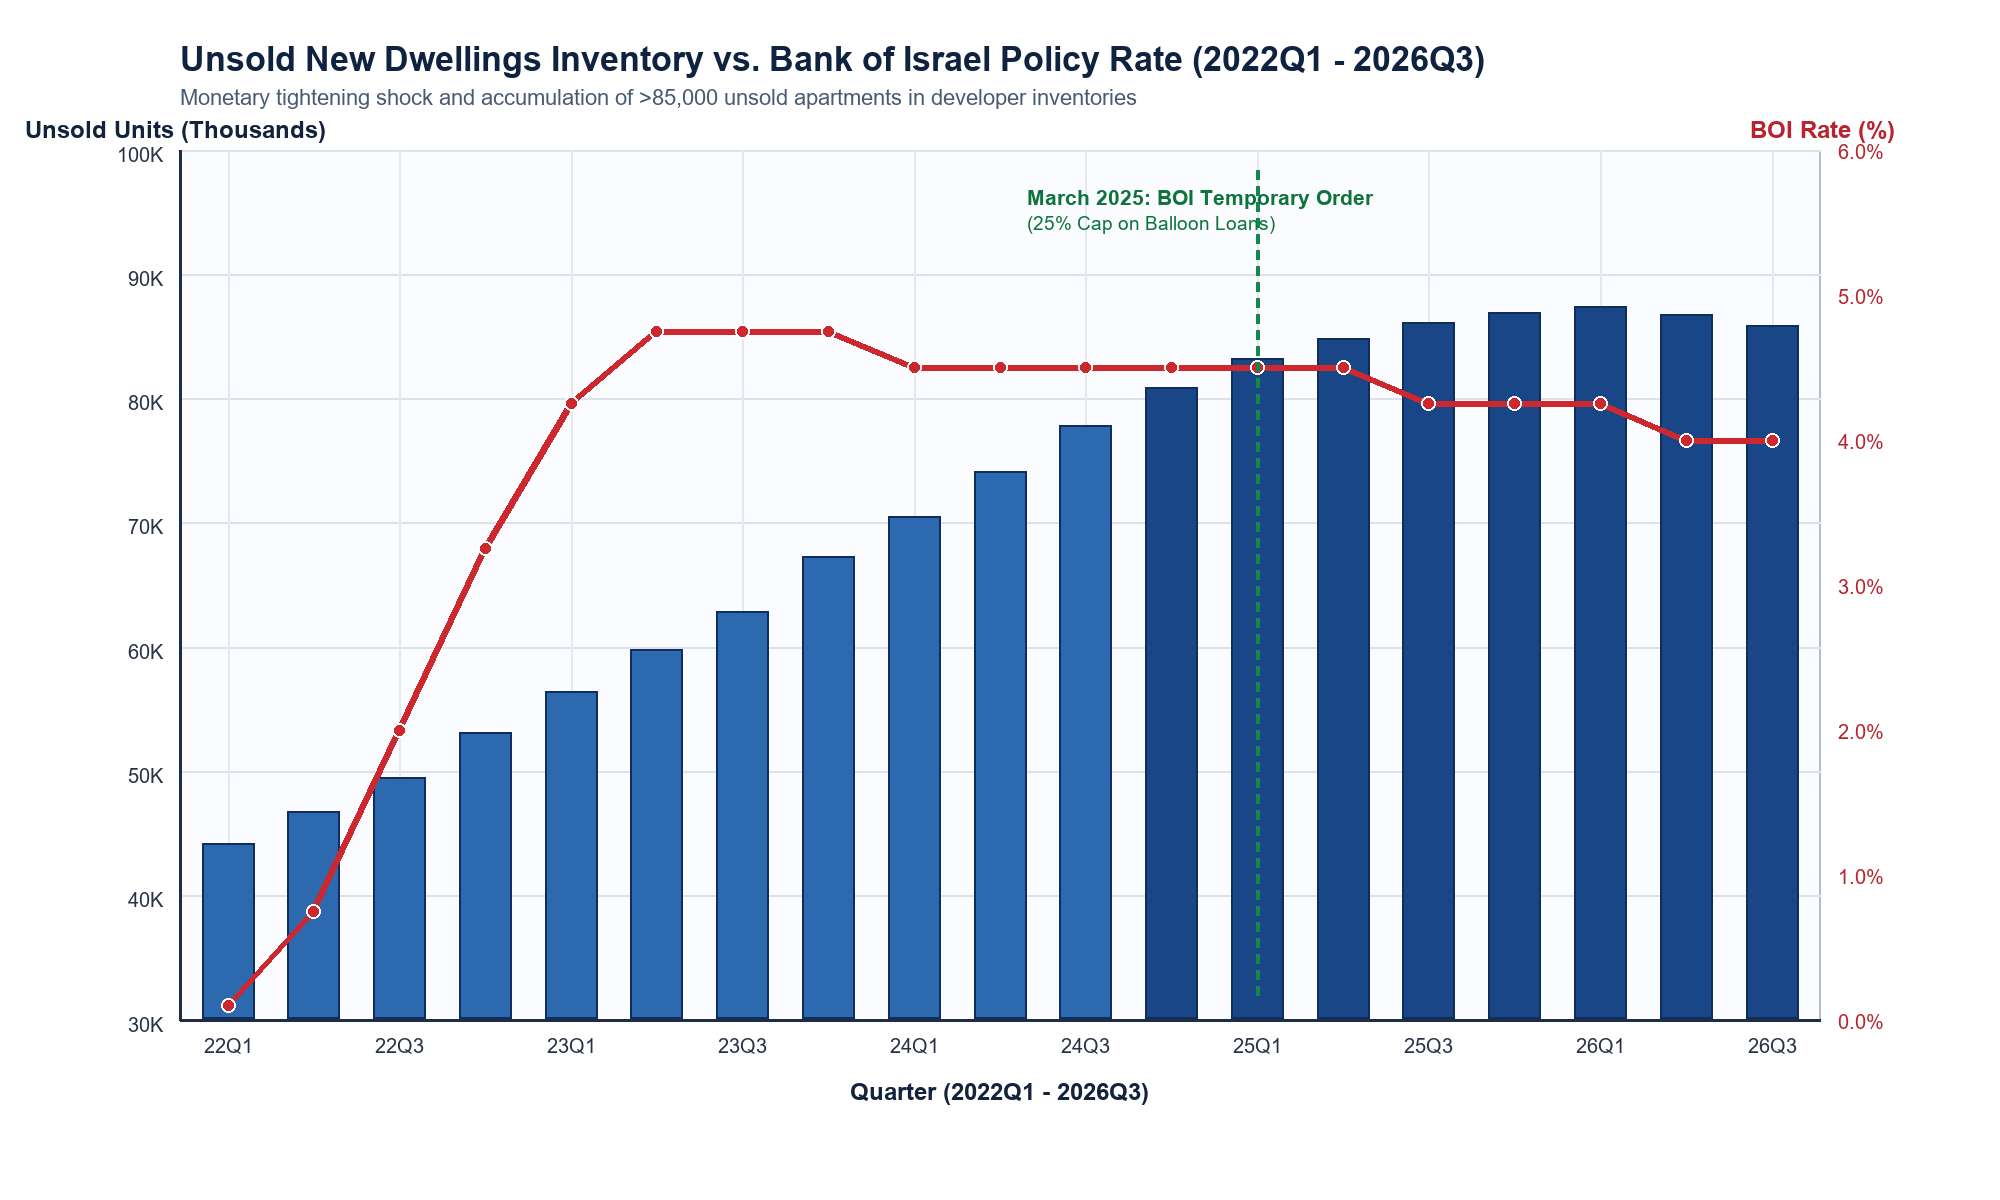
\includegraphics[width=0.96\textwidth]{fig03_israel_inventory_vs_rates.png}
\caption{התפתחות מלאי הדירות החדשות הלא-מכורות בישראל (באלפי יח"ד, ציר שמאל) מול נתיב ריבית בנק ישראל (באחוזים, ציר ימין) בשנים \num{2022}--\num{2026}: זינוק המלאי מ-\num{44,200} יח"ד לשיא של \num{87,400} יח"ד והתייצבות מעל \num{85,000} יח"ד \cite{cbs2026dwellings,boi2025stability}}
\label{fig:israel_inventory_rates}
\end{figure}

איור~\ref{fig:israel_inventory_rates} מציג את התוצאה המאקרו-כלכלית של כוחות אלו. בעוד שקצב מכירת הדירות החדשות צנח ב-\num{2023} בכ-\pct{42} לעומת שיא \num{2021}, התחלות הבנייה של פרויקטים שתוכננו ומומנו בשנות הגאות המשיכו להיכנס לצנרת הביצוע. כתוצאה מכך, מלאי הדירות החדשות הלא-מכורות שבידי הקבלנים זינק מ-\num{44,200} דירות ברבעון הראשון של \num{2022} ל-\num{67,900} דירות בסוף \num{2023}, חצה לראשונה את רף ה-\num{80,000} בסוף \num{2024}, והגיע לשיא היסטורי של \textbf{\num{87,400} דירות לא-מכורות} ברבעון הראשון של \num{2026} (ו-\num{85,900} יח"ד ברבעון השלישי של \num{2026} — שווה-ערך לכ-\num{28.5} חודשי היצע בקצב המכירות השוטף) \cite{cbs2026dwellings}.

\section{פילוח שוק תלת-שכבתי (\en{TAM / SAM / SOM}) של חשיפת מבצעי הקבלן}
\label{sec:tam_sam_som}

בהתאם להנחיות פרק \num{6.1} בספר \en{"}מהבעיה אל ה-\en{PDF}\en{"} \cite{segal2026prep}, אפיון מדויק של היקף התופעה הכלכלית מחייב פילוח כמותי תלת-שכבתי: השוק הכולל (\en{TAM -- Total Addressable Market}), השוק הנגיש (\en{SAM -- Serviceable Available Market}) ופלח השוק בר-המימוש העומד במוקד הסיכון של המחקר (\en{SOM -- Serviceable Obtainable Market}). איור~\ref{fig:tam_sam_som} וטבלה~\ref{tab:tam_sam_som} מציגים את הכימות המדויק של שלוש השכבות בשוק הדיור והאשראי הישראלי בשנים \num{2022}--\num{2026}.

\begin{figure}[htbp]
\centering
\begin{english}
\begin{tikzpicture}[font=\small]
    % Outer TAM Box
    \draw[fill=BrandLightBlue, draw=BrandNavy, line width=1.3pt, rounded corners=8pt] (0,0) rectangle (14.4,5.6);
    \node[anchor=north west, font=\normalsize\bfseries, color=BrandNavy] at (0.35, 5.3) {TAM -- Total Addressable Market (\texthebrew{כלל שוק עסקאות הדיור בישראל 2022--2026})};
    \node[anchor=north west, font=\small, color=BrandNavy] at (0.35, 4.75) {\texthebrew{היקף מצרפי: \num{385,000} עסקאות דיור (חדשות + יד שנייה) בשווי כולל של כ-\nis{885} מיליארד (\usd{242B})}};

    % Middle SAM Box
    \draw[fill=BrandLightTeal, draw=BrandTeal, line width=1.3pt, rounded corners=7pt] (0.6,0.35) rectangle (13.8,4.15);
    \node[anchor=north west, font=\normalsize\bfseries, color=BrandTeal] at (0.95, 3.85) {SAM -- Serviceable Available Market (\texthebrew{שוק הדירות החדשות מקבלן ומלאי לא-מכור})};
    \node[anchor=north west, font=\small, color=BrandTeal] at (0.95, 3.30) {\texthebrew{\num{148,000} דירות חדשות שנמכרו + \num{85,900} דירות לא-מכורות בביצוע; שווי מצרפי כ-\nis{584} מיליארד (\usd{160B})}};

    % Inner SOM Box
    \draw[fill=BrandLightRed, draw=BrandRed, line width=1.5pt, rounded corners=6pt] (1.2,0.70) rectangle (13.2,2.65);
    \node[anchor=north west, font=\normalsize\bfseries, color=BrandRed] at (1.55, 2.38) {SOM -- Target Risk Cohort (\texthebrew{פלח המטרה במחקר: עסקאות מבצעי מימון ובלון בקיר המסירות})};
    \node[anchor=north west, font=\small, color=BrandRed] at (1.55, 1.82) {\texthebrew{\textbf{\num{54,200} משקי בית} שרכשו במבצעי \num{20/80}, \num{10/90}, \num{20/50/30} והלוואות בלון (\num{2023}--\num{2026})}};
    \node[anchor=north west, font=\small\bfseries, color=BrandRed] at (1.55, 1.25) {\texthebrew{חוב נדחה לפירעון במועד המסירה (\num{2026}--\num{2027}): כ-\nis{108.4} מיליארד (\usd{29.7B}) + אשראי יזמי ממונף של כ-\nis{68} מיליארד}};
\end{tikzpicture}
\end{english}
\caption{פילוח שוק תלת-שכבתי (\en{TAM / SAM / SOM}) של שוק הדיור הישראלי ופלח הסיכון של מבצעי הקבלנים לקראת קיר המסירות (\num{2026}--\num{2027}) \cite{segal2026prep,cbs2026dwellings,boi2025stability}}
\label{fig:tam_sam_som}
\end{figure}

\begin{table}[htbp]
\caption{כימות שכבות השוק (\en{TAM / SAM / SOM}) ביחידות דיור, בשקלים חדשים ובדולרים (\num{2022}--\num{2026}) \cite{cbs2026dwellings,boi2025stability,mof2025economist}}
\label{tab:tam_sam_som}
\centering
\small
\renewcommand{\arraystretch}{1.28}
\rowcolors{2}{BrandGray}{white}
\begin{tabularx}{\textwidth}{R{1.8cm} R{3.2cm} R{2.2cm} R{2.3cm} Y}
\toprule
\rowcolor{TableHeaderBg}
\textbf{שכבה} & \textbf{הגדרת הפלח האנליטי} & \textbf{היקף ביח"ד} & \textbf{שווי מצרפי} & \textbf{משמעות מתודולוגית למחקר} \\
\midrule
\textbf{\en{TAM}} & כלל עסקאות הדיור בישראל (יד ראשונה + יד שנייה, \num{2022}--\num{2026}) & \num{385,000} יח"ד & \nis{885B} (\usd{242B}) & מסגרת המאקרו לקביעת מדדי מחירים, עומק אשראי לדיור (\nis{565B}) ויציבות בנקאית. \\
\textbf{\en{SAM}} & סקטור הבנייה החדשה (דירות שנמכרו \en{"}על הנייר\en{"} + מלאי לא-מכור של \num{85.9K}) & \num{233,900} יח"ד & \nis{584B} (\usd{160B}) & זירת הפעילות של חברות הבנייה וחשיפת האשראי הבנקאי והחוץ-בנקאי לביצוע ולקרקע. \\
\textbf{\en{SOM}} & עסקאות מבצעי מימון (\num{20/80}, \num{10/90}, \num{20/50/30}, בלון קבלן) המסתימות ב-\num{2026}--\num{2027} & \num{54,200} יח"ד & \nis{135.5B} שווי חוזי (\nis{108.4B} חוב נדחה) & \textbf{אוכלוסיית היעד של הסימולציות:} משקי הבית והיזמים שיעמדו למבחן סילוק היתרה בקיר המסירות. \\
\bottomrule
\end{tabularx}
\end{table}

\section{התפתחות מבצעי המימון: מ-\num{20/80} דרך התערבות בנק ישראל ועד מוטציות \num{20/50/30}}
\label{sec:promotions_evolution}

ניתוח כרונולוגי של שוק הראשוני בישראל בשנים \num{2022}--\num{2026} חושף אבולוציה בת שלושה שלבים במבנה חוזי המכר הקבלניים, המשקפת משחק אסטרטגי מתמשך בין היזמים לבין הפיקוח על הבנקים \cite{boi2025stability,boi2025directive,mof2025economist}:

\subsection{שלב א' (\num{2022Q4}--\num{2024Q4}): פריצת מבצעי \num{20/80}, \num{10/90} והלוואות בלון מסובסדות}
כדי להניע רוכשים לחתום על חוזים למרות זינוק הריבית, החלו הקבלנים בסוף \num{2022} להחליף את לוח התשלומים החוקי הקלאסי (שבו הרוכש משלם בשיעורים מדורגים לפי קצב התקדמות הבנייה וצמוד למדד תשומות הבנייה) בשני מנגנונים משולבים:
\begin{enumerate}[label=\textbf{\arabic*.},rightmargin=0.6cm]
  \item \textbf{דחיית תשלום ליניארית (\num{20/80}, \num{15/85}, \num{10/90} ואף \num{5/95}):} הרוכש משלם במועד החתימה \pct{10} עד \pct{20} בלבד ממחיר הדירה מההון העצמי, ופטור מכל תשלום נוסף עד לקבלת טופס \num{4} ומסירת המפתח (\num{36}--\num{42} חודשים קדימה). יתרת ה-\pct{80}--\pct{90} נדחית לתשלום אחד במועד המסירה, לרוב תוך מתן \textbf{פטור מלא או חלקי מהצמדה למדד תשומות הבנייה} על היתרה הנדחית.
  \item \textbf{הלוואת קבלן / הלוואת בלון מסובסדת (\en{Subsidized Bullet Loan}):} בפרויקטים שבהם הבנק המלווה דרש תזרים מזומנים לחשבון הליווי כבר בעת החתימה, הרוכש נטל הלוואת גישור בנקאית (\en{Bullet / Balloon}) של \pct{40}--\pct{75} משווי הדירה לתקופת הבנייה, כאשר \textbf{היזם משלם לבנק את מלוא תשלומי הריבית השוטפים} במקום הרוכש עד למועד המסירה \cite{boi2025stability,boi2025directive}. במועד המסירה פוקעת הלוואת הבלון, והרוכש נדרש לפרוע אותה באמצעות נטילת משכנתא רגילה בריבית השוק או ממכירת הדירה.
\end{enumerate}

\subsection{שלב ב' (מרץ \num{2025}): התערבות הפיקוח על הבנקים (הוראת השעה)}
לאחר ששיעור עסקאות המימון בערים מובילות חצה ברבעון הרביעי של \num{2024} את רף ה-\pct{45} מהעסקאות בדירות חדשות \cite{mof2025economist}, פרסם הפיקוח על הבנקים במרץ \num{2025} הוראת שעה מחייבת שנועדה לצנן את החשיפה המערכתית \cite{boi2025directive}. הוראת השעה קבעה שני בלמים כמותיים:
\begin{itemize}[rightmargin=0.6cm]
  \item \textbf{תוספת הקצאת הון על ליווי פרויקטים עתירי דחייה:} בפרויקטי בנייה שבהם למעלה מ-\pct{25} מחוזי המכר כוללים דחיית תשלום ליניארית (שבה שיעור התשלום במועד המסירה עולה על \pct{80} או שלוח התשלומים אינו תואם את קצב התקדמות הבנייה), חויבו הבנקים להגדיל את משקל הסיכון (\en{Risk Weight}) להקצאת הון בגין אשראי הליווי של הפרויקט.
  \item \textbf{תקרה כמותית של \pct{10} על הלוואות בלון מסובסדות:} היקף הלוואות הגישור (\en{Bullet/Balloon}) לדיור שבהן הקבלן מסבסד את הריבית הוגבל ל-\pct{10} לכל היותר מסך הביצועים החודשיים של משכנתאות חדשות בכל בנק \cite{boi2025directive}.
\end{itemize}

\subsection{שלב ג' (\num{2025Q2}--\num{2026Q4}): מוטציות עוקפות רגולציה (\num{20/50/30} ואשראי חוץ-בנקאי)}
התגובה בשוק לא הייתה הורדת מחירי המחירון של הדירות, אלא פיתוח מהיר של \textbf{מוטציות חוזיות עוקפות רגולציה} שתוכננו לעמוד פורמלית בתנאי הוראת השעה של בנק ישראל תוך שימור דחיית התשלום בפועל עבור הרוכש:
\begin{enumerate}[label=\textbf{\arabic*.},rightmargin=0.6cm]
  \item \textbf{מבנה מדורג סינתטי (\num{20/50/30} ו-\num{15/55/30}):} כדי שחוזה המכר לא יסווג כעסקה שבה \pct{80} משולמים במסירה (ובכך יפגע במכסת ה-\pct{25} של פרויקט הליווי הבנקאי), החוזה מחולק ל-\pct{20} בחתימה, \pct{50} באמצע תקופת הבנייה (למשל בחודש ה-\num{18} או ה-\num{20}), ו-\pct{30} במסירה. בפועל, עבור תשלום הביניים של ה-\pct{50}, היזם מעמיד לרוכש הלוואת גישור דרך גוף מימון חוץ-בנקאי או חברת ביטוח שותפה, או מעניק זכות דחייה חוזית מותנית עד למסירה.
  \item \textbf{הלוואות רוכשים חוץ-בנקאיות (\en{Non-Bank Buyer Bullet}):} מכיוון שמגבלת ה-\pct{10} של בנק ישראל חלה על המערכת הבנקאית בלבד, קרנות אשראי חוץ-בנקאיות וגופים מוסדיים נכנסו לוואקום והעמידו הלוואות בלון במימון של \pct{85}--\pct{90} לרוכשי דירות \en{"}על הנייר\en{"} בריביות גבוהות המסובסדות על ידי היזם מתוך תקציב השיווק של הפרויקט.
\end{enumerate}

\section{המנגנון הכלכלי והמתמטי: \en{"}מחיר מדף\en{"} נומינלי מול הנחת \en{NPV} סמויה}
\label{sec:npv_hidden_discount}

מדוע יזמי הנדל"ן בישראל מוכנים לספוג עלויות מימון וויתור על הצמדה למדד בשווי של מאות אלפי שקלים לדירה במקום להפחית ישירות את מחיר הדירה הנומינלי ב-\pct{8}--\pct{12}? התשובה טמונה במבנה המוסדי של \textbf{חשבון הליווי הבנקאי הסגור ודוח האפס}:

בליווי בנקאי סגור בישראל, הבנק מעמיד ליזם קו אשראי לביצוע הפרויקט בכפוף לשני תנאים פיננסיים קשיחים (\en{Financial Covenants}): (א) שמירה על שיעור רווח יזמי מינימלי חזוי בדוח האפס (לרוב \pct{15}--\pct{18} מהעלויות); ו-(ב) עמידה בקצב מכירות מינימלי במחיר ממוצע למ"ר שאינו נופל ממחיר הבסיס בדוח השמאי (\en{Zero Report}) \cite{boi2024annual,salelaw1974}. אם יזם מוריד רשמית את מחיר המחירון של דירה מ-\num{3.00} מיליון ש"ח ל-\num{2.70} מיליון ש"ח (\pct{-10}), שמאי הפרויקט מחויב לעדכן כלפי מטה את שווי כלל המלאי הלא-מכור בפרויקט. עדכון זה מוחק מיידית את כרית הרווח היזמי בדוח הליווי ומחייב את הבנק לדרוש מהיזם \textbf{הזרמת הון עצמי מיידית במזומן (\en{Equity Cure})} — מזומן שאין ליזמים ממונפים. לעומת זאת, כאשר היזם מוכר את הדירה במחיר חוזי נקוב (\en{Headline Price}) של \num{3.00} מיליון ש"ח במבצע \num{20/80} או בהלוואת בלון מסובסדת, המחיר הנומינלי נשמר בדוח המכירות ובדיווח לרשות המסים, בעוד שעלות הסבסוד נרשמת כ\en{"}הוצאות מימון ושיווק\en{"} הנפרסות לאורך חיי הפרויקט.

\subsection{פיתוח נוסחת הנחת הערך הנוכחי הנקי (\en{Implicit NPV Discount})}
נגדיר מתמטית את שיעור ההנחה הכלכלית הסמויה הגלומה במבצעי המימון. נסמן ב-$P_{\text{nom}}$ את מחיר החוזה הנומינלי של הדירה, וב-$T$ את תקופת הבנייה בשנים עד למסירה ($T = 3.0$ שנים, או \num{36} חודשים). בעסקת רכישה תקנית הצמודה לקצב הבנייה (\en{Benchmark Standard Contract}), הרוכש משלם סדרת תשלומים $\{\alpha_k P_{\text{nom}}\}_{k=1}^{K}$ במועדים $t_k \in [0, T]$ ($\sum_{k=1}^K \alpha_k = 1$), כאשר כל תשלום עתידי צמוד למדד תשומות הבנייה בקצב שנתי $\pi_c$, ומהוון לפי עלות ההון האלטרנטיבית / ריבית המימון השנתית $r$. הערך הנוכחי הנקי של התשלומים בעסקה תקנית (בהנחה שגם בה \pct{20} הראשונים משולמים ב-$t=0$ והיתרה נפרסת באופן שווה לאורך הבנייה) הוא:
\begin{equation}
\label{eq:pv_standard}
\text{PV}_{\text{std}} = P_{\text{nom}} \left[ \alpha_0 + \sum_{k=1}^{K} \alpha_k \left(\frac{1 + \pi_c}{1 + r}\right)^{t_k} \right]
\end{equation}

לעומת זאת, בעסקת מבצע קבלן עם דחיית תשלום ליניארית ($\alpha_0 \in \{0.10, 0.20\}$ בחתימה, ויתרה של $1 - \alpha_0$ במועד המסירה $T$ עם פטור מלא מהצמדה למדד תשומות הבנייה $\pi_c = 0$ על היתרה הנדחית), הערך הנוכחי הכלכלי שהרוכש משלם (והיזם מקבל במונחי ערך נוכחי לפני עלות מימון הבנק) הוא:
\begin{equation}
\label{eq:pv_promo}
\text{PV}_{\text{promo}}\left(\alpha_0, r, T\right) = P_{\text{nom}} \left[ \alpha_0 + \frac{1 - \alpha_0}{\left(1 + r\right)^T} \right]
\end{equation}

שיעור הנחת ה-\en{NPV} האפקטיבית הסמויה ($\delta_{\text{NPV}}$) לעומת מחיר המחירון המוצהר בעסקה צמודת-מדד מוגדר על ידי משוואה~\eqref{eq:npv_discount_rate}:
\begin{equation}
\label{eq:npv_discount_rate}
\delta_{\text{NPV}}\left(\alpha_0, r, \pi_c, T\right) = 1 - \frac{\alpha_0 + \left(1 - \alpha_0\right)\left(1 + r\right)^{-T}}{\alpha_0 + \left(1 - \alpha_0\right)\left(\frac{1 + \pi_c}{1 + r}\right)^{T/2}}
\end{equation}

\begin{figure}[htbp]
\centering
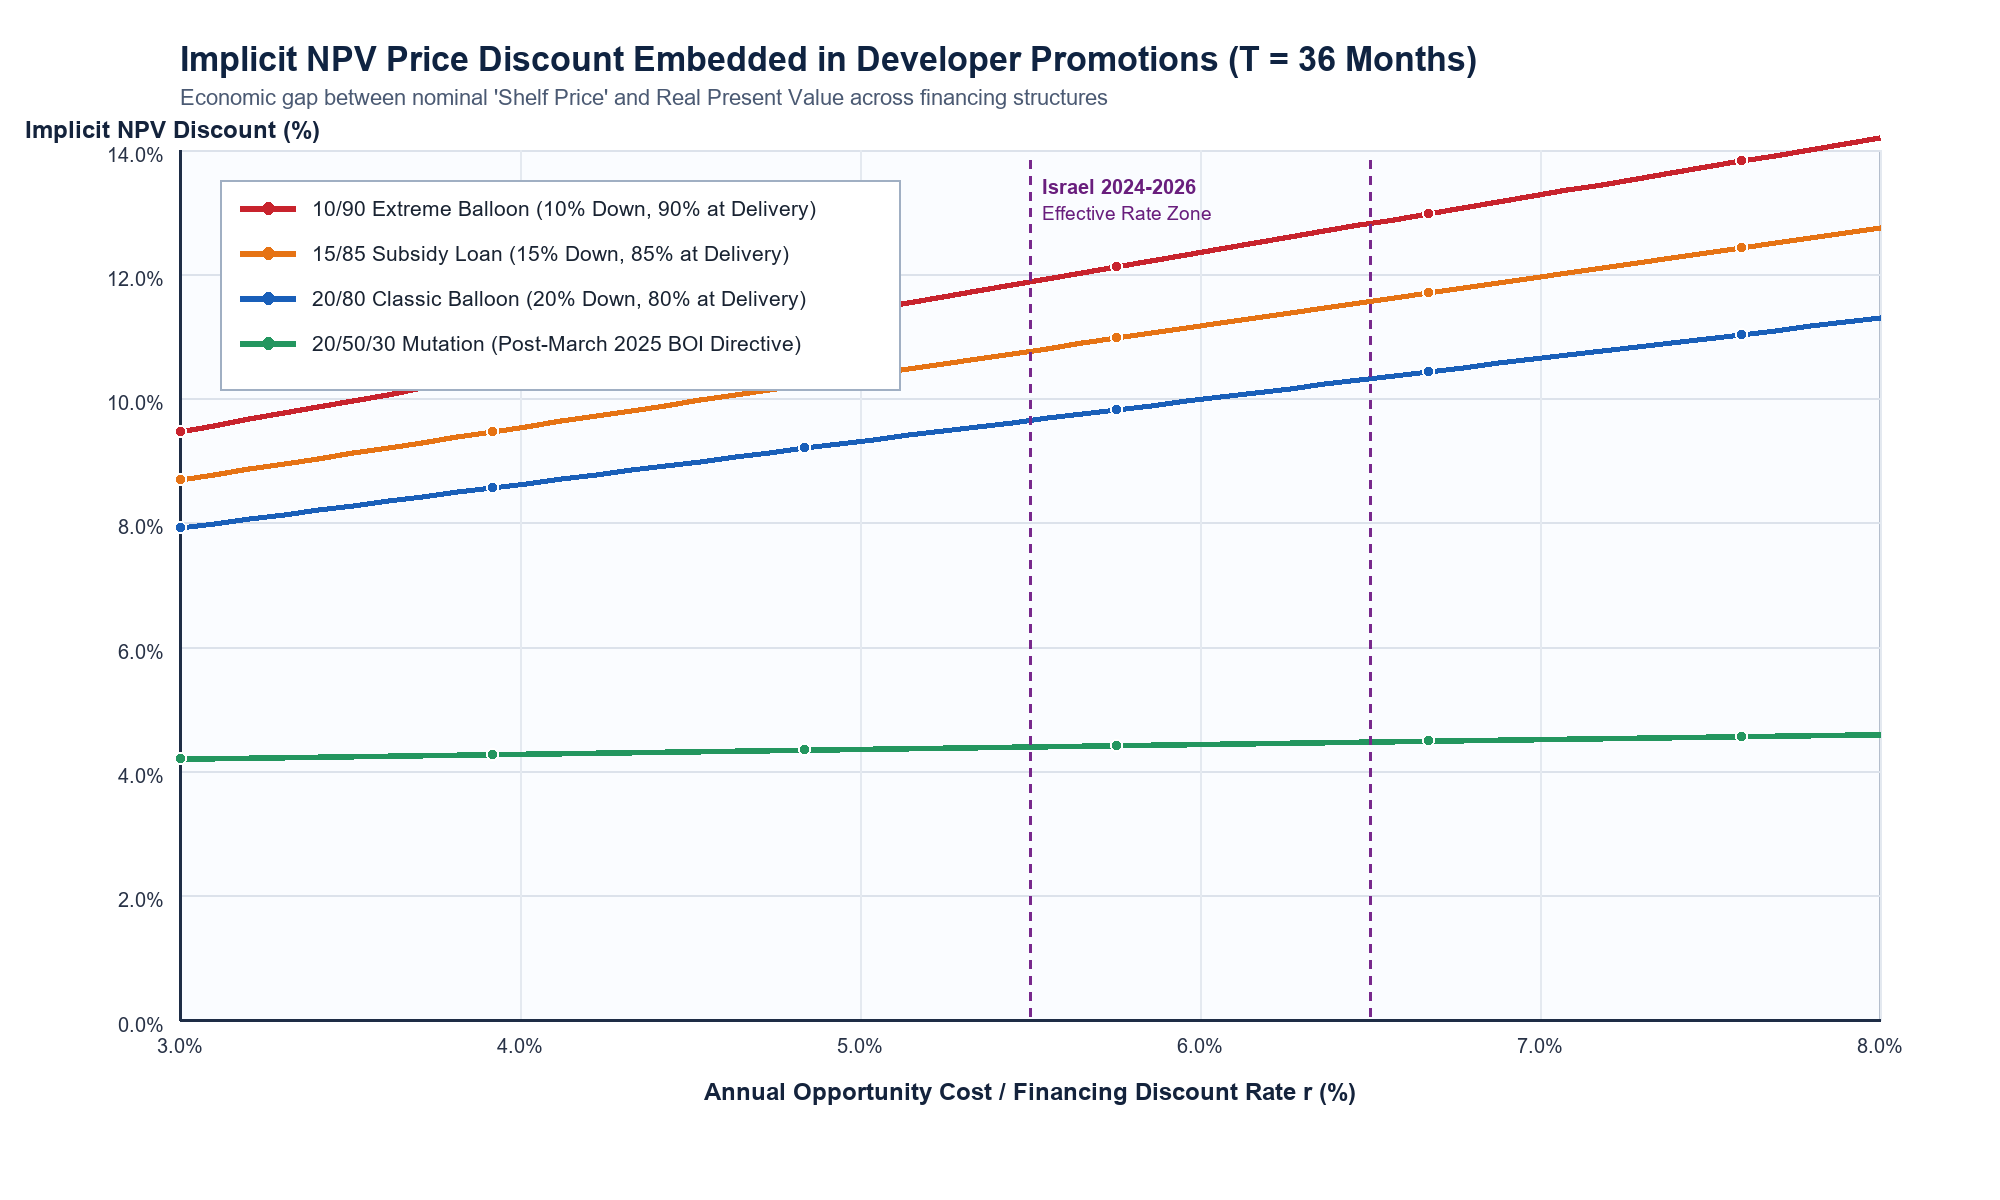
\includegraphics[width=0.95\textwidth]{fig01_npv_discount_curves.png}
\caption{עקומות שיעור ההנחה הכלכלית הסמויה (\en{Implicit NPV Discount}, $\delta_{\text{NPV}}$) כפונקציה של ריבית ההיוון השנתית ($r$) עבור שלוש ארכיטקטורות מבצעי מימון (\num{10/90}, \num{20/80} ומוטציית \num{20/50/30}) לתקופת מסירה של $T=36$ חודשים ופטור ממדד תשומות בנייה של $\pi_c=2.5\%$ לשנה}
\label{fig:npv_discount_curves}
\end{figure}

איור~\ref{fig:npv_discount_curves} וטבלה~\ref{tab:israel_promotions_anatomy} מציגים את תוצאות המודל המתמטי מתוך הרצת הסימולציה בפייתון (\en{\texttt{scripts/run\_simulations\_and\_figures.py}}). בסביבת ריבית מימון אפקטיבית של $r = 6.0\%$ לשנה ואינפלציית מדד תשומות בנייה של $\pi_c = 2.5\%$ לשנה למשך $T = 36$ חודשים:
\begin{itemize}[rightmargin=0.6cm]
  \item עסקת \textbf{\num{20/80}} מגלמת הנחת מחיר אמיתית סמויה של \textbf{\pct{9.99}} (כ-\nis{280,000} על דירה שמחירה החוזי \num{2.80} מיליון ש"ח).
  \item עסקת \textbf{\num{10/90}} (או הלוואת בלון של \pct{90} בריבית מסובסדת במלואה על ידי הקבלן) מגלמת הנחת מחיר סמויה של \textbf{\pct{12.36}} (כ-\nis{346,000} לדירה).
  \item מוטציית \textbf{\num{20/50/30}} שלאחר הוראת השעה של בנק ישראל מגלמת הנחה סמויה של \textbf{\pct{4.44}} כאשר תשלום ה-\pct{50} משולם בפועל באמצע התקופה ($t=18$ חודשים), אך שבה וחוצה את רף ה-\textbf{\pct{9.2}} כאשר תשלום הביניים ממומן באמצעות הלוואת בלון חוץ-בנקאית על חשבון היזם.
\end{itemize}

\begin{table}[htbp]
\caption{אנטומיה השוואתית של מבצעי המימון הקבלניים בישראל (\num{2022}--\num{2026}): מבנה תזרימי, הנחת \en{NPV} סמויה ומוקד סיכון ב\en{"}קיר המסירות\en{"}}
\label{tab:israel_promotions_anatomy}
\centering
\small
\renewcommand{\arraystretch}{1.28}
\rowcolors{2}{BrandGray}{white}
\begin{tabularx}{\textwidth}{R{2.5cm} R{2.8cm} R{1.9cm} R{2.1cm} Y}
\toprule
\rowcolor{TableHeaderBg}
\textbf{מבנה העסקה} & \textbf{פריסת תשלומים (חתימה / ביניים / מסירה)} & \textbf{הנחת \en{NPV} ($\mathbf{r=6\%}$)} & \textbf{חיתום בנקאי לרוכש בחתימה} & \textbf{מנגנון הכשל הפוטנציאלי בקיר המסירות (\num{2026}--\num{2027})} \\
\midrule
\textbf{חוזה תקני (ייחוס)} & \pct{20} / \pct{60} מדורג / \pct{20} (צמוד מדד תשומות) & \pct{0.00} & מלא (נטילת משכנתא מדורגת) & סיכון נמוך: יכולת ההחזר נבדקה והמשכנתא נלקחה ברובה לאורך הבנייה. \\
\textbf{ליניארי \num{20/80} (פטור ממדד)} & \pct{20} בחתימה / \pct{0} בביניים / \pct{80} במסירה & \pct{9.99} & חלקי בלבד (לרוב אישור עקרוני לא מחייב) & \textbf{הלם החזר (\en{Payment Shock}):} הרוכש נדרש לגייס \pct{80} במשכנתא אחת בריבית גבוהה בעת המסירה. \\
\textbf{קיצון \num{10/90} / \num{15/85}} & \pct{10}--\pct{15} בחתימה / \pct{0} בביניים / \pct{85}--\pct{90} במסירה & \pct{12.36} & היעדר חיתום מחייב; משקיעי \en{"}פליפ\en{"} & \textbf{מלכודת \en{LTV} ו-\en{PTI}:} משקיע או משפר דיור שמוגבל ל-\pct{50}--\pct{70} משכנתא אינו יכול להשלים את העסקה ללא מכירה. \\
\textbf{הלוואת בלון קבלן מסובסדת} & \pct{15}--\pct{20} הון עצמי + \pct{65}--\pct{80} בלון בנקאי בריבית על חשבון היזם & \pct{9.80}--\pct{11.50} & חיתום בנקאי מראש על הלוואת הגישור & \textbf{סיכון מחזור (\en{Rollover Risk}):} פקיעת הבלון במסירה מחייבת מעבר להחזר חודשי מלא של קרן וריבית. \\
\textbf{מוטציית \num{20/50/30} (אחרי מרץ \num{2025})} & \pct{20} בחתימה / \pct{50} בחודש \num{18} (בלון חוץ-בנקאי) / \pct{30} במסירה & \pct{4.44} (או \pct{9.20} בסיבסוד חוץ-בנקאי) & עוקף את מגבלת ה-\pct{25} וה-\pct{10} של בנק ישראל & \textbf{זליגת סיכון לאשראי חוץ-בנקאי:} מינוף כפול של הרוכש והיזם מול קרנות מימון פרטיות בריבית גבוהה. \\
\bottomrule
\end{tabularx}
\end{table}

\begin{warningbox}[העיוות הסטטיסטי והמימוני הכפול של מבצעי הקבלן]
הניתוח המתמטי בפרק זה חושף כי מבצעי המימון הקבלניים בשנים \num{2022}--\num{2026} ייצרו שני עיוותים מערכתיים במקביל:
\begin{enumerate}[label=\textbf{\arabic*.},rightmargin=0.5cm]
  \item \textbf{עיוות מדידת האינפלציה ומדד מחירי הדירות:} מאחר שהלמ"ס ורשות המסים קולטים את מחיר החוזה הנומינלי ($P_{\text{nom}}$) ללא ניכוי הנחת ה-\en{NPV} הסמויה ($\delta_{\text{NPV}} \approx 10\%$), מדד מחירי הדירות הרשמי בשנים \num{2023}--\num{2025} הציג יציבות או עלייה מדומה בשעה שהמחיר הכלכלי הריאלי בשוק הראשוני ירד \cite{mof2025economist,ita2025carman}.
  \item \textbf{דחיית החיתום הבנקאי האמיתי למועד האכלוס (\en{Deferred Underwriting}):} בעסקאות \num{20/80} ו-\num{10/90} ליניאריות (שאינן מבוססות על הלוואת בלון בנקאית שנחתמה מראש), הרוכש אינו נוטל משכנתא במועד החתימה. בדיקת כושר ההחזר המחייבת לפי יחס ה-\en{PTI} והערכת שמאי הבנק למשכנתאות נדחות ב-\num{36} חודשים למועד המסירה (\num{2026}--\num{2027}) — בדיוק בנקודת הזמן שבה מצטברות מעל \num{85,000} דירות לא-מכורות מתחרות.
\end{enumerate}
\end{warningbox}

% ==============================================================================
% chapters/ch04_comparative_analysis.tex
% פרק ד': ניתוח השוואתי – ישראל 2026 מול ארה"ב 2008 והסיכונים הגלומים
% ==============================================================================

\chapter{ניתוח השוואתי – ישראל \num{2026} מול ארה"ב \num{2008} והסיכונים הגלומים}
\label{ch:comparative_analysis}

לאחר שניתחנו בפרק ב' את מנגנוני הכשל של משבר הסאב-פריים האמריקאי (\num{2001}--\num{2008}) ובפרק ג' את התפתחות מבצעי המימון הקבלניים בישראל (\num{2022}--\num{2026}), פרק זה מעמיד את שני השווקים למבחן השוואתי שיטתי. בהתאם למתודולוגיית הניתוח ההשוואתי הרב-ממדי בפרק \num{6.2} ו-\num{6.3} בספר \en{"}מהבעיה אל ה-\en{PDF}\en{"} \cite{segal2026prep}, אנו נמנעים מהקבלה שטחית (\en{"}ישראל היא סאב-פריים \num{2.0}\en{"} או מנגד \en{"}בישראל הכל בטוח\en{"}), ומפרקים את ההשוואה לעשרה פרמטרים כמותיים ומוסדיים. הניתוח מראה כי בעוד שבמישור המיקרו-כלכלי של עיצוב החוזה והתנהגות הרוכש קיים דמיון מדאיג למשבר \num{2008}, הרי שבמישור המאקרו-יציבותי והמשפטי ניצבים בישראל ארבעה \en{"}שוברי גלים\en{"} מוסדיים החוסמים התפתחות של קריסה בנקאית מערכתית, אך מנתבים את מלוא הלחץ אל חוליה פגיעה אחרת: **המגזר היזמי הממונף באשראי חוץ-בנקאי ומשקי הבית בבקבוק המסירות**.

\section{מוקדי הדמיון (אזורי הסכנה): אשליית ההון העצמי, הימור הריבית וניגוד העניינים}
\label{sec:similarities_danger}

השוואה מבנית בין חוזי ה-\en{Hybrid ARM} וה-\en{Option ARM} בארה"ב (\num{2004}--\num{2006}) לבין חוזי ה-\num{20/80}, ה-\num{10/90} והלוואות הבלון בישראל (\num{2022}--\num{2026}) מעלה שלושה מנגנוני כשל משותפים המהווים את \en{"}חומר הבעירה\en{"} בשני השווקים:

\begin{enumerate}[label=\textbf{\arabic*.},rightmargin=0.6cm]
  \item \textbf{אשליית הון עצמי נמוך וכניסת רוכשים שוליים (\en{Marginal Buyers}):} בארה"ב אפשרו הלוואות ה-\en{Piggyback 80/20} רכישת בית עם \pct{0}--\pct{5} הון עצמי \cite{mayer2009rise}. בישראל, אף שהוראות בנק ישראל מחייבות הון עצמי של \pct{25}--\pct{50} בעת נטילת המשכנתא הסופית \cite{boi2025stability}, מבצעי ה-\num{10/90} וה-\num{15/85} אפשרו למשקי בית ולמשקיעים להיכנס לעסקה חוזית מחייבת על נכס בשווי \num{2.8}--\num{3.5} מיליון ש"ח באמצעות העמדת מקדמה ראשונית של \num{280}--\num{420} אלף ש"ח בלבד. בכך נוצר מינוף חוזי אפקטיבי של \num{1:7} עד \num{1:10} על ההון העצמי לאורך תקופת הבנייה.
  \item \textbf{הימור ספקולטיבי על ירידת ריבית או עסקת \en{"}פליפ\en{"} לפני המסירה:} כפי שהוכיחו \en{Gorton (2009)} \cite{gorton2009securitized} ו-\en{Mayer et al. (2009)} \cite{mayer2009rise}, הלוואת ה-\en{2/28 ARM} בארה"ב נלקחה מתוך הנחה שהלווה ימחזר את החוב או ימכור את הבית ברווח לפני איפוס הריבית בחודש \num{24}. באופן זהה לחלוטין, פלח משמעותי מרוכשי ה-\num{20/80} וה-\num{10/90} בישראל בשנים \num{2023}--\num{2025} חתם על החוזים תחת שתי הנחות ספקולטיביות: (א) שריבית בנק ישראל תצנח בחזרה ל-\pct{1.5}--\pct{2.0} עד מועד המסירה ב-\num{2026}--\num{2027}; או (ב) שניתן יהיה להמחות את הזכויות (\en{Assignment / Flip}) לקונה אחר ברווח הון לפני מועד התשלום הסופי. כאשר שתי ההנחות מתבדות מול מלאי שיא של \num{85,900} דירות חדשות מתחרות, האופציה הספקולטיבית פוקעת מחוץ לכסף.
  \item \textbf{ניגוד עניינים של יזמים ומשווקים וניפוח מחיר החוזה (\en{Price Distortion}):} עבודתו של \en{Ben-David (2011)} \cite{ben2011inflated} על שוק הסאב-פריים האמריקאי תיעדה כיצד מוכרים העניקו תמריצים כספיים לקונים דלי-הון כדי לנפח מלאכותית את מחיר העסקה המדווח ולחלץ אשראי גבוה יותר מהבנק. בישראל (\num{2022}--\num{2026}), מנגנון זה שוחזר בקנה מידה תעשייתי: שימור \en{"}מחיר המדף\en{"} הנומינלי תוך סבסוד הלוואת הבלון או ויתור על מדד תשומות הבנייה ($\delta_{\text{NPV}} \approx 10\%--12.4\%$) נועד למנוע הפחתת שווי בדוחות השמאות של הליווי הבנקאי הסגור.
\end{enumerate}

\section{מוקדי השוני: ארבעת \en{"}שוברי הגלים\en{"} המוסדיים של ישראל}
\label{sec:differences_shields}

למרות הדמיון המיקרו-כלכלי במבנה החוזים הדחויים, ניתוח מוסדי ומשפטי מעלה ארבעה הבדלים מבניים תהומיים בין ארצות הברית של \num{2008} לבין ישראל של \num{2026}, המוצגים במטריצה ההשוואתית המלאה בטבלה~\ref{tab:us_vs_israel_comparison}.

\begin{table}[htbp]
\caption{מטריצה השוואתית רב-ממדית: ארה"ב במשבר הסאב-פריים (\num{2001}--\num{2008}) מול שוק הדיור והאשראי בישראל (\num{2022}--\num{2026}) \cite{mian2009consequences,keys2010did,ghent2011recourse,boi2025stability,boi2025directive,salelaw1974}}
\label{tab:us_vs_israel_comparison}
\centering
\footnotesize
\renewcommand{\arraystretch}{1.26}
\rowcolors{2}{BrandGray}{white}
\begin{tabularx}{\textwidth}{R{2.3cm} Y Y R{2.1cm}}
\toprule
\rowcolor{TableHeaderBg}
\textbf{ממד השוואה} & \textbf{ארה"ב (\num{2001}--\num{2008} – משבר הסאב-פריים)} & \textbf{ישראל (\num{2022}--\num{2026} – מבצעי קבלן וקיר המסירות)} & \textbf{כיוון ההשפעה על היציבות בישראל} \\
\midrule
\textbf{1. חוזה המימון המרכזי} & משכנתאות \en{Hybrid 2/28 \& 3/27 ARM}, \en{Option ARM (Neg-Am)} והלוואות \en{Interest-Only}. & דחיית תשלום ליניארית (\num{20/80}, \num{10/90}), מוטציית \num{20/50/30} והלוואות בלון קבלן מסובסדות. & \textbf{\color{BrandGold}סיכון דומה} (דחיית הלם ההחזר ל-\num{36} חודשים). \\
\textbf{2. הון עצמי בחתימה ומגבלת \en{LTV}} & הון עצמי אפסי (\pct{0}--\pct{5}); מינוף מצרפי \en{CLTV} של \pct{95}--\pct{100} באמצעות \en{Piggyback 80/20}. & \pct{10}--\pct{20} בחתימה על החוזה, אך תקרת \en{LTV} קשיחה של בנק ישראל במשכנתא: \pct{75} / \pct{70} / \pct{50}. & \textbf{\color{BrandTeal}יתרון לישראל} לבנקים; \textbf{\color{BrandRed}סיכון סגירה} לרוכש במסירה. \\
\textbf{3. חיתום ואימות הכנסה (\en{PTI})} & מעל \pct{50} הלוואות \en{Low/No-Doc} ו-\en{NINJA}; היעדר תקרת יחס החזר להכנסה מחייבת. & אימות הכנסה מלא ותקרת \en{PTI} קשיחה (\pct{40}--\pct{50}), אך בעסקאות ליניאריות החיתום נדחה למסירה. & \textbf{\color{BrandTeal}מגן חזק לבנקים}; חושף רוכשים לדחיית משכנתא במסירה. \\
\textbf{4. משטר משפטי (\en{Recourse})} & \textbf{\en{Non-Recourse}} במדינות מפתח: הלווה מוסר את המפתח לבנק (\en{Put Option}) ופטור מיתרת החוב. & \textbf{\en{Full Personal Recourse}}: אחריות אישית מלאה של הרוכש + פיצוי מוסכם (\pct{10}--\pct{15}) ליזם בביטול חוזה. & \textbf{\color{BrandTeal}מגן קריטי}: מונע נטישה אסטרטגית (\en{Jingle Mail}). \\
\textbf{5. איגוח ומודל החזקת הסיכון} & \textbf{\en{Originate-to-Distribute}}: מכירת ההלוואות ל-\en{RMBS}, \en{CDO} ו-\en{CDS} במינוף \en{Repo} קצר-מועד. & \textbf{\en{Originate-to-Hold}}: המשכנתאות מוחזקות במלואן במאזני הבנקים המסחריים; אפס איגוח סאב-פריים. & \textbf{\color{BrandTeal}מגן מערכתי}: אין הדבקת בנקאות צללים ונגזרים. \\
\textbf{6. ליווי בנייה והגנת הרוכש} & היעדר חוק מכר פדרלי אחיד; קבלנים ספקולטיביים בנו ללא ליווי סגור וערבויות אישיות לרוכש. & \textbf{חוק המכר (\num{1974})}: חשבון ליווי בנקאי סגור (\en{Ring-Fenced}) וערבות חוק מכר בנקאית לכל שקל ששולם. & \textbf{\color{BrandTeal}מגן מוסדי}: מבודד פרויקטים ומונע אובדן מקדמות. \\
\textbf{7. מינוף יזמים ואשראי חוץ-בנקאי} & חברות בנייה מומנו באשראי בנקאי ושוק ההון עם יכולת מחיקת אופציות קרקע. & יזמים קטנים/בינוניים במינוף קרקע של \pct{70}--\pct{85} ואשראי \textbf{מזנין חוץ-בנקאי} בריבית \en{Prime+5\%--8\%}. & \textbf{\color{BrandRed}מוקד פגיעות חריף בישראל} (\en{Tier-2/Tier-3}). \\
\textbf{8. כריות ההון של המערכת הבנקאית} & בנקי השקעות במינוף \num{1:30}--\num{1:40} (הון עצמי מוחשי של \pct{2.5}--\pct{3.5}); בנקים מסחריים עם כריות דקות. & חמישה בנקים ריכוזיים תחת פיקוח הדוק עם יחס הון עצמי רובד \num{1} (\textbf{\en{CET1}}) של \textbf{\pct{10.6}--\pct{10.9}}. & \textbf{\color{BrandTeal}עמידות גבוהה}: כרית ספיגת הפסדים רחבה מאוד. \\
\bottomrule
\end{tabularx}
\end{table}

\subsection{ניתוח מתמטי של אפקט ה-\en{Full Recourse} וחוק המכר בישראל מול ארה"ב}
ההבדל המכריע ביותר בהתנהגות משקי הבית טמון במשטר ה-\en{Full Recourse} בישראל לעומת ה-\en{Non-Recourse} בארה"ב \cite{ghent2011recourse}. כפי שהראינו במשוואה~\eqref{eq:non_recourse_put} בפרק ב', בארה"ב ברגע שמחיר הדירה $P_T$ ירד מתחת ליתרת החוב $L_T$, הלווה מימש את אופציית הנטישה ומסר את המפתח לבנק.

לעומת זאת, בישראל חוזה הרכישה מול הקבלן וחוזה המשכנתא מול הבנק מקימים חבות אישית מלאה (\en{Full Personal Liability}). אם רוכש דירה במבצע \num{20/80} (ששילם מקדמה $\alpha_0 P_{\text{nom}}$ במועד החתימה ונותר חייב $\left(1-\alpha_0\right)P_{\text{nom}}$ במועד המסירה $T$) מבקש להפר את החוזה וליטוש את העסקה עקב ירידת שווי השוק של הדירה ל-$P_T < P_{\text{nom}}$, היזם (והבנק המלווה) רשאים לחלט פיצוי מוסכם קבוע בחוזה בשיעור $\kappa \in [0.10, 0.15]$ ממלוא מחיר החוזה $P_{\text{nom}}$, ובנוסף לתבוע את הפרש הירידה בשווי הנכס מתוך נכסיו האישיים והכנסתו העתידית של הרוכש. לפיכך, תנאי הכדאיות הכלכלית לנטישה אסטרטגית מרצון בישראל דורש:
\begin{equation}
\label{eq:israel_recourse_condition}
\text{Loss}_{\text{complete}}\left(T\right) = P_{\text{nom}} - P_T + \text{PV}\left(\Delta M_{\text{mortgage}}\right) > \kappa P_{\text{nom}} + \theta_{\text{recourse}}\max\left(P_{\text{nom}}\left(1-\kappa\right) - P_T,\, 0\right) + C_{\text{legal}}
\end{equation}
כאשר $\theta_{\text{recourse}} \approx 1$ מייצג את שיעור הגבייה האפקטיבי בהליכי הוצאה לפועל מול משק בית בעל הכנסה או נכסים בישראל. ממשוואה~\eqref{eq:israel_recourse_condition} נובעת תוצאה אנליטית מרכזית: **בישראל אין לרוכש אופציית \en{Put} חינמית על הדירה**. גם אם מחיר הדירה בשוק ירד ב-\pct{10}--\pct{12}, רוכש ישראלי לא \en{"}יזרוק את המפתחות\en{"} מרצונו החופשי, אלא יעשה כל מאמץ למכור את הדירה בשוק המשני (אף בהפסד של רוב ההון העצמי שהפקיד), לגייס הלוואות משפחתיות או לפרוס את המשכנתא ל-\num{30} שנה — וייקלע לחדלות פירעון אך ורק כאשר נחסמת בפניו רגולטורית האפשרות לקבל משכנתא מהבנק (\en{Inability to Close}) וגם נכשלה מכירת הדירה לצד שלישי (\en{Double Liquidity Lock}).

\begin{figure}[htbp]
\centering
\begin{english}
\begin{tikzpicture}
\begin{axis}[
    xbar,
    width=13.8cm,
    height=7.8cm,
    xmin=0, xmax=10.5,
    ytick={1,2,3,4,5,6,7},
    yticklabels={
        {\textbf{7. Bank Capital Thinness (CET1)}},
        {\textbf{6. Securitization Contagion (CDO/Repo)}},
        {\textbf{5. Strategic Default Risk (Non-Recourse)}},
        {\textbf{4. Underwriting Laxity (NINJA/No-Doc)}},
        {\textbf{3. Developer \& Mezzanine Leverage}},
        {\textbf{2. Price-to-Income \& Affordability Stretch}},
        {\textbf{1. Deferred Payment Shock (ARM / 20-80)}}
    },
    xlabel={\textbf{Systemic Vulnerability Score (1 = Minimal Risk, 10 = Extreme Vulnerability)}},
    bar width=7.5pt,
    grid=major,
    grid style={dashed, gray!35},
    legend style={at={(0.5,1.08)}, anchor=south, legend columns=2, font=\small, draw=BrandNavy},
    nodes near coords,
    nodes near coords style={font=\scriptsize\bfseries},
    enlarge y limits=0.12
]
\addplot[fill=BrandRed!80, draw=BrandRed] coordinates {
    (8.8,1) (7.5,2) (6.8,3) (9.5,4) (9.2,5) (9.8,6) (9.0,7)
};
\addlegendentry{US Subprime Crisis (2007--2008)}

\addplot[fill=BrandBlue!80, draw=BrandNavy] coordinates {
    (8.4,1) (8.9,2) (8.6,3) (3.8,4) (2.2,5) (1.2,6) (2.5,7)
};
\addlegendentry{Israel Housing \& Delivery Wall (2026--2027)}
\end{axis}
\end{tikzpicture}
\end{english}
\caption{פרופיל פגיעות השוואתי רב-ממדי (ציון \num{1}--\num{10}): ארה"ב במשבר הסאב-פריים (\num{2007}--\num{2008}) מול ישראל לקראת קיר המסירות (\num{2026}--\num{2027}) בשבעה ממדי סיכון מערכתיים \cite{segal2026prep,boi2025stability}}
\label{fig:comparative_risk_profile}
\end{figure}

\section{מפת הסיכונים הייחודית לישראל: היכן כן עלול להיווצר כשל בקיר המסירות?}
\label{sec:israel_unique_risk_map}

פרופיל הפגיעות ההשוואתי באיור~\ref{fig:comparative_risk_profile} מדגים בבירור את האסימטריה של המקרה הישראלי: בעוד שבארה"ב ציוני הפגיעות היו גבוהים מאוד (\num{8.8}--\num{9.8}) בממדי האיגוח, היעדר החיתום, משטר ה-\en{Non-Recourse} ודקות ההון הבנקאי, בישראל ממדים אלו מוגנים היטב (ציוני פגיעות נמוכים של \num{1.2}--\num{3.8}). לעומת זאת, ישראל מציגה פגיעות גבוהה במיוחד — ואף חמורה יותר מארה"ב — בשלושה מוקדים ספציפיים המרכיבים את **מפת קווי השבר של \num{2026}--\num{2027}** (איור~\ref{fig:israel_fault_line_map}):

\begin{figure}[htbp]
\centering
\begin{english}
\begin{tikzpicture}[
    node distance=0.55cm and 0.6cm,
    faultbox/.style={
        rectangle,
        rounded corners=4pt,
        draw=BrandRed,
        line width=1.1pt,
        fill=BrandLightRed,
        text width=4.4cm,
        minimum height=2.3cm,
        align=center,
        font=\footnotesize
    },
    shieldbox/.style={
        rectangle,
        rounded corners=4pt,
        draw=BrandTeal,
        line width=1.2pt,
        fill=BrandLightTeal,
        text width=14.2cm,
        minimum height=1.2cm,
        align=center,
        font=\small
    },
    corebox/.style={
        rectangle,
        rounded corners=4pt,
        draw=BrandNavy,
        line width=1.2pt,
        fill=BrandLightBlue,
        text width=14.2cm,
        minimum height=1.1cm,
        align=center,
        font=\small\bfseries
    },
    arrow/.style={-{Stealth[length=2.6mm,width=2.0mm]}, line width=1.1pt, color=BrandRed},
    blockarrow/.style={-{Bar[width=4mm,line width=1.5pt]}, line width=1.2pt, color=BrandTeal}
]
    \node[faultbox] (f1) {\textbf{\color{BrandRed}Fault Line A: Buyers}\\[3pt]\texthebrew{רוכשי \num{20/80} ו-\num{10/90} שנדחים במבחן \en{PTI > 40\%} או משפרי דיור שנתקעו עם דירתם הישנה}};
    \node[faultbox, right=of f1] (f2) {\textbf{\color{BrandRed}Fault Line B: Inventory}\\[3pt]\texthebrew{\num{85,900} דירות חדשות לא-מכורות מתחרות המונעות מכירת \en{"}פליפ\en{"} ברווח לפני טופס \num{4}}};
    \node[faultbox, right=of f2] (f3) {\textbf{\color{BrandRed}Fault Line C: Tier-3 Devs}\\[3pt]\texthebrew{יזמים קטנים/בינוניים במינוף קרקע ומזנין חוץ-בנקאי (\en{Prime+6\%}) עם \en{DSCR < 1.0}}};

    \node[shieldbox, below=0.75cm of f2] (shield) {\textbf{\color{BrandTeal}Israeli Institutional Firewall (Sale Law + BOI LTV/PTI + Full Recourse + CET1 10.85\%)}\\[2pt]\texthebrew{בולמת הדבקה מערכתית לבנקים, אך כולאת את ההפסד אצל היזמים הממונפים, קרנות המזנין וההון העצמי של הרוכשים}};

    \node[corebox, below=0.55cm of shield] (bank) {\color{BrandNavy}Commercial Banking Core Stability Preserved (\texthebrew{יציבות המערכת הבנקאית נשמרת: \en{CET1 > 9.38\%} גם בתרחיש קיצון})};

    \draw[arrow] (f1.south) -- ([xshift=-4.8cm]shield.north);
    \draw[arrow] (f2.south) -- (shield.north);
    \draw[arrow] (f3.south) -- ([xshift=4.8cm]shield.north);
    \draw[blockarrow] (shield.south) -- (bank.north);
\end{tikzpicture}
\end{english}
\caption{מפת קווי השבר הייחודית לישראל לקראת קיר המסירות (\num{2026}--\num{2027}): מיקוד הכשל בשלוש חוליות הקצה ובלימת ההדבקה המערכתית על ידי חומת האש המוסדית \cite{boi2025stability,salelaw1974}}
\label{fig:israel_fault_line_map}
\end{figure}

\begin{enumerate}[label=\textbf{\arabic*.},rightmargin=0.6cm]
  \item \textbf{קו שבר א' – מלכודת משפרי הדיור והמשקיעים הממונפים (\en{Double Asset Lock}):} משפרי דיור שרכשו דירה חדשה במבצע \num{15/85} או בהלוואת בלון קבלן מתוך כוונה למכור את דירתם הקיימת סמוך למועד המסירה ב-\num{2026}--\num{2027}, מגלים כי שוק היד השנייה קפוא לחלוטין עקב התחרות מול מבצעי הקבלנים ומלאי ה-\num{85,900} דירות. ללא מכירת הדירה הישנה, הם חסומים רגולטורית מנטילת משכנתא מעל \pct{50}--\pct{70} וחשופים לקנס מס רכישה ולהפרת חוזה.
  \item \textbf{קו שבר ב' – יזמים קטנים ובינוניים (\en{Tier-2 / Tier-3}) הממונפים באשראי מזנין חוץ-בנקאי:} כדי להעמיד את ההון העצמי שנדרש על ידי הבנקים המלווים (\pct{20}--\pct{25} מעלות הפרויקט), יזמים רבים נטלו הלוואות השלמת הון (\en{Mezzanine}) מקרנות אשראי חוץ-בנקאיות בריבית של \pct{11}--\pct{14} (\en{Prime + 5\%--8\%}). בפרויקטים אלו, הבנק המלווה מובטח בשעבוד ראשון על הפרויקט, אך עיכוב של \num{6}--\num{12} חודשים בתקבולי המסירה או גל ביטולים של \pct{15}--\pct{20} מהחוזים מוחק לחלוטין את עודפי הפרויקט וגורם לחדלות פירעון של היזם ושל קרנות המזנין.
  \item \textbf{קו שבר ג' – משקי בית בעשירוני הביניים שנדחקים מעבר לתקרת ה-\en{PTI} במועד המסירה:} רוכשים שחתמו על עסקאות \num{20/80} ליניאריות ללא משכנתא מאושרת מראש ונדרשים לגייס במועד המסירה משכנתא של \num{1.8}--\num{2.4} מיליון ש"ח בריבית של \pct{5.5}, כאשר ההחזר החודשי חוצה את רף ה-\pct{40}--\pct{50} מהכנסתם הפנויה והבנק המסחרי מסרב להעמיד את ההלוואה.
\end{enumerate}

\begin{managerbox}[סיכום פרק ד' לקובעי המדיניות: הבחנה בין סיכון מערכתי לסיכון סקטוריאלי]
הניתוח ההשוואתי בפרק זה מוביל למסקנה אסטרטגית חדה: ישראל של \num{2026} אינה עומדת בפני \en{"}משבר ליהמן ברדרס\en{"} של קריסת בנקים מסחריים, בזכות חומת האש המשולשת של חוק המכר, הוראות ה-\en{LTV/PTI} של בנק ישראל ומשטר ה-\en{Full Recourse}. אולם עצם עוצמתה של חומת האש הבנקאית משמעותה ש\textbf{הבנקים מוגנים על ידי העברת מלוא הלם הנזילות אל החוליות החלשות בשרשרת}: רוכשי \en{"}על הנייר\en{"} שייאלצו למכור דירות במחירי מצוקה לפני טופס \num{4}, יזמי נדל"ן ממונפים שייקלעו לכינוס נכסים, וגופי אשראי חוץ-בנקאיים שהעמידו הלוואות מזנין ובלון ללא כריות ביטחון מספקות. פרק ה' ופרק ו' יכמתו בדיוק מתמטי את עוצמת הפגיעה בכל אחת מחוליות אלו.
\end{managerbox}

% ==============================================================================
% chapters/ch05_methodology_and_data.tex
% פרק ה': מתודולוגיה, מקורות נתונים וארכיטקטורה אנליטית
% ==============================================================================

\chapter{מתודולוגיה, מקורות נתונים וארכיטקטורה אנליטית}
\label{ch:methodology}

פרק זה מתרגם את שאלות המחקר, ההשערות ($H_1, H_2, H_3$) ודרישות המערכת הכמותיות (\en{REQ-RES-01} עד \en{REQ-RES-08} שהוגדרו בפרק א') לארכיטקטורה מתודולוגית ואנליטית בת-ביצוע. בהתאם להנחיות פרק \num{7} בספר \en{"}מהבעיה אל ה-\en{PDF}\en{"} \cite{segal2026prep}, אנו פותחים בהצגת מאגרי הנתונים האמפיריים, ממשיכים בבחירה הנדסית מנומקת בין שלוש חלופות מתודולוגיות באמצעות **מטריצת החלטה משוקללת (\en{Weighted Pugh Decision Matrix})** ובדיקת רגישות למשקולות \cite{pugh1991total,segal2026prep}, מפתחים בשלמותם את המודלים המתמטיים לסימולציית משקי הבית, היזמים והבנקים, ומציגים את תרשים הבלוקים של מערכת הסימולציה בפייתון (\en{Python}) ו-\en{RStudio}.

\section{מאגרי הנתונים האמפיריים ושיטות טיוב המידע}
\label{sec:data_sources}

כדי להתגבר על העובדה שהלמ"ס ורשות המסים אינם מפרסמים שדה מובנה של \en{"}שיעור הנחת קבלן\en{"} בכל עסקה, המחקר מצליב ארבעה מאגרי נתונים רשמיים משלימים לשנים \num{2022}--\num{2026}, המפורטים בטבלה~\ref{tab:data_sources_schema}:

\begin{table}[htbp]
\caption{מערך מאגרי הנתונים האמפיריים של המחקר: מקורות, משתנים נחלצים, היקף מדגם ושיטת כיול \cite{ita2025carman,cbs2026dwellings,boi2025stability,mof2025economist}}
\label{tab:data_sources_schema}
\centering
\footnotesize
\renewcommand{\arraystretch}{1.26}
\rowcolors{2}{BrandGray}{white}
\begin{tabularx}{\textwidth}{R{2.3cm} R{2.8cm} R{2.2cm} Y R{2.4cm}}
\toprule
\rowcolor{TableHeaderBg}
\textbf{מאגר נתונים} & \textbf{גוף מפרסם ורזולוציה} & \textbf{היקף תצפיות (\num{2022}--\num{2026})} & \textbf{משתנים כמותיים מרכזיים נחלצים} & \textbf{אתגר מדידה ושיטת טיוב} \\
\midrule
\textbf{1. מאגר כרמ"ן וסקירות האוצר} & רשות המסים ואגף הכלכלן הראשי (עסקאות פרטניות) & כ-\num{148,000} עסקאות דירות חדשות & מחיר חוזי מוצהר ($P_{\text{nom}}$), תאריך עסקה, תאריך מסירה חזוי, גוש/חלקה, וסוג רוכש (דירה יחידה / משפר / משקיע). & מחיר חוזי אינו מנכה הטבות מימון; מכויל מול תזרים קבלנים לפי מודל ה-\en{NPV}. \\
\textbf{2. סדרות בנייה ומלאי דירות} & הלשכה המרכזית לסטטיסטיקה (הלמ"ס – חודשי/רבעוני) & \num{19} רבעונים (\num{2022Q1}--\num{2026Q3}) & התחלות וגמר בנייה, מלאי דירות חדשות לא-מכורות (\num{87.4K} שיא), חודשי היצע (\num{28.5}), ומדד תשומות הבנייה ($\pi_c$). & פיגור דיווח ברבעון האחרון; מתוקנן מול קצב היתרי בנייה וטופס \num{4}. \\
\textbf{3. דוחות פיקוח ויציבות בנקאית} & בנק ישראל – חטיבת המחקר והפיקוח על הבנקים & \num{5} קבוצות בנקאיות (\pct{98} מהשוק) & ביצועי משכנתאות לפי מסלול, שיעור הלוואות בולט/בלון, התפלגות \en{LTV} ו-\en{PTI}, יחס הון \en{CET1}, והפרשות להפסדי אשראי. & נתונים מקובצים לעשירוני סיכון; משמשים לכיול פרמטרי של התפלגות מונטה-קרלו. \\
\textbf{4. דוחות כספיים בורסאיים (מאי"ה)} & בורסת ת"א (\en{TASE}) – דוחות שנתיים ורבעוניים מבוקרים & \num{25} חברות יזמיות (\en{Tier 1/2/3}) & יחס חוב ל-\en{CAP}, שיעור גבייה מרוכשים מראש (\pct{15}--\pct{22}), יתרות אשראי ליווי ומזנין, הוצאות מימון ורווח גולמי מפרויקטים. & הטיה לחברות ציבוריות; שכבת \en{Tier-3} מכוילת לפי פרויקטים במימון קרנות חוץ-בנקאיות. \\
\bottomrule
\end{tabularx}
\end{table}

\section{חלופות תכן מתודולוגיות ומטריצת החלטה משוקללת (\en{Pugh Matrix})}
\label{sec:pugh_matrix}

לפני נעילת הארכיטקטורה האנליטית של המחקר, נבחנו שלוש חלופות מתודולוגיות מובחנות (בהתאם לכלל \en{"}שלוש חלופות אמיתיות\en{"} בפרק \num{7.1} בספר של ד"ר סגל \cite{segal2026prep}):
\begin{enumerate}[label=\textbf{\arabic*.},rightmargin=0.6cm]
  \item \textbf{חלופה א' (\en{Alt A} – אקונומטריקה מאקרו-כלכלית מצרפית \en{VAR/OLS}):} אמידת מודל אוטו-רגרסיבי וקטורי (\en{Vector Autoregression}) על סדרות עתיות רבעוניות מצרפיות של מחירי דירות, ריבית בנק ישראל ושיעור הפיגורים במשכנתאות. \textbf{יתרון:} פשטות חישובית וזמינות נתונים מיידית. \textbf{חיסרון קריטי:} עיוורון מוחלט לזנב ההתפלגות המיקרו-כלכלי (רוכשי ה-\num{10/90} ויזמי ה-\en{Tier-3}), וחוסר יכולת למדל אירוע לא-ליניארי עתידי כגון \en{"}קיר המסירות\en{"}.
  \item \textbf{חלופה ב' (\en{Alt B} – ניתוח חשבונאי השוואתי של מקרי בוחן יזמיים \en{Case-Study Accounting}):} ניתוח עומק של דוחות כספיים ודוחות אפס של \num{5}--\num{8} חברות בנייה נבחרות בלבד. \textbf{יתרון:} דיוק חשבונאי גבוה ברמת הפרויקט הבודד. \textbf{חיסרון קריטי:} היעדר יכולת הכללה סטטיסטית לאוכלוסיית \num{54,200} משקי הבית וחוסר חיבור למודל הלימות ההון (\en{CET1}) של המערכת הבנקאית.
  \item \textbf{חלופה ג' (\en{Alt C} – ארכיטקטורה היברידית: סימולציית מונטה-קרלו מיקרו-כלכלית + מבחני קיצון מאזניים תלת-שכבתיים – החלופה הנבחרת):} שילוב של מודל תמחור מהוון (\en{NPV}), סימולציית מונטה-קרלו סטוכסטית ($N=10,000$ משקי בית) לאמידת הלם ההחזר ושיעור החריגה מתקרת ה-\en{PTI}, והזנת שיעור הכשל המתקבל לתוך מודל מבחני קיצון (\en{Stress Test}) ליחס כיסוי החוב (\en{DSCR}) של שלוש שכבות יזמים (\en{Tiers 1--3}) וליחס הון \en{CET1} של הבנקים.
\end{enumerate}

ציון ההחלטה המשוקלל $S_j$ עבור כל חלופה $j \in \{A, B, C\}$ מחושב לפי משוואת פיו (\en{Pugh Weighted Sum}) \cite{pugh1991total,segal2026prep}:
\begin{equation}
\label{eq:pugh_score}
S_j = \sum_{i=1}^{6} w_i \cdot c_{ij}, \qquad \text{subject to} \quad \sum_{i=1}^{6} w_i = 1.00, \quad c_{ij} \in [1, 10]
\end{equation}
כאשר $w_i$ הוא משקל החשיבות של קריטריון $i$ ו-$c_{ij}$ הוא הציון ההנדסי של חלופה $j$ בקריטריון $i$. טבלה~\ref{tab:pugh_decision_matrix} ואיור~\ref{fig:pugh_scores_chart} מציגים את תוצאות הדירוג.

\begin{table}[htbp]
\caption{מטריצת החלטה משוקללת (\en{Pugh Matrix}) לבחירת הארכיטקטורה המתודולוגית של המחקר (לפי פרק \num{7.2} בספר \en{"}מהבעיה אל ה-\en{PDF}\en{"} \cite{segal2026prep,pugh1991total})}
\label{tab:pugh_decision_matrix}
\centering
\small
\renewcommand{\arraystretch}{1.25}
\rowcolors{2}{BrandGray}{white}
\begin{tabularx}{\textwidth}{Y C{1.5cm} C{2.2cm} C{2.2cm} C{2.5cm}}
\toprule
\rowcolor{TableHeaderBg}
\textbf{קריטריון הערכה מתודולוגי ($i$)} & \textbf{משקל ($w_i$)} & \textbf{חלופה א': מאקרו \en{VAR/OLS}} & \textbf{חלופה ב': מקרי בוחן חשבונאיים} & \textbf{חלופה ג' (נבחרת): היברידית \en{MC + Stress}} \\
\midrule
1. יכולת זיהוי סיכוני זנב מיקרו-כלכליים (\en{Payment Shock}) & \pct{25} & \num{4.0} (\num{1.00}) & \num{6.0} (\num{1.50}) & \textbf{\num{9.5} (\num{2.375})} \\
2. קישור אנליטי בין משקי בית, יזמים (\en{DSCR}) ובנקים (\en{CET1}) & \pct{20} & \num{5.0} (\num{1.00}) & \num{6.5} (\num{1.30}) & \textbf{\num{9.5} (\num{1.900})} \\
3. יכולת ניטרול הטיית מחיר החוזה הנומינלי (\en{NPV Adjustment}) & \pct{15} & \num{4.5} (\num{0.675}) & \num{7.5} (\num{1.125}) & \textbf{\num{9.0} (\num{1.350})} \\
4. תקפות אמפירית והתאמה לנתוני הלמ"ס, בנק ישראל ומאי"ה & \pct{15} & \num{8.0} (\num{1.20}) & \num{7.0} (\num{1.05}) & \textbf{\num{9.0} (\num{1.350})} \\
5. עמידות להנחות וניתוח רגישות רב-תרחישי (\num{10\%/20\%/30\%}) & \pct{15} & \num{6.5} (\num{0.975}) & \num{6.0} (\num{0.90}) & \textbf{\num{9.0} (\num{1.350})} \\
6. ישימות חישובית בלוח הזמנים של הסמסטר (\num{14} שבועות) & \pct{10} & \num{9.5} (\num{0.95}) & \num{8.5} (\num{0.85}) & \textbf{\num{7.5} (\num{0.750})} \\
\midrule
\rowcolor{TableHeaderBg}
\textbf{ציון משוקלל כולל ($S_j = \sum w_i c_{ij}$)} & \textbf{\pct{100}} & \textbf{\num{5.80} / \num{10}} & \textbf{\num{6.73} / \num{10}} & \textbf{\color{BrandTeal}\num{9.08} / \num{10} (נבחרה)} \\
\bottomrule
\end{tabularx}
\end{table}

\begin{figure}[htbp]
\centering
\begin{english}
\begin{tikzpicture}
\begin{axis}[
    ybar,
    width=13.5cm,
    height=6.2cm,
    ymin=0, ymax=10.5,
    symbolic x coords={Alt A: Macro VAR/OLS, Alt B: Case-Study Accounting, Alt C: Hybrid MC + Stress Test},
    xtick=data,
    ylabel={\textbf{Weighted Decision Score ($S_j$, Scale 1--10)}},
    bar width=28pt,
    grid=major,
    grid style={dashed, gray!35},
    nodes near coords,
    nodes near coords style={font=\small\bfseries, color=BrandNavy},
    title={\textbf{\color{BrandNavy}Weighted Pugh Matrix Comparison of Methodological Alternatives}}
]
\addplot[fill=BrandBlue!75, draw=BrandNavy, line width=1.1pt] coordinates {
    (Alt A: Macro VAR/OLS, 5.80)
    (Alt B: Case-Study Accounting, 6.73)
    (Alt C: Hybrid MC + Stress Test, 9.08)
};
\draw[dashed, color=BrandTeal, line width=1.2pt] (axis cs:Alt A: Macro VAR/OLS,8.0) -- (axis cs:Alt C: Hybrid MC + Stress Test,8.0);
\node[anchor=south west, font=\footnotesize\bfseries, color=BrandTeal] at (axis cs:Alt A: Macro VAR/OLS, 8.1) {Approval Threshold (8.0)};
\end{axis}
\end{tikzpicture}
\end{english}
\caption{השוואת הציונים המשוקללים של שלוש חלופות התכן המתודולוגיות במטריצת פיו (\en{Pugh Matrix}): עליונות מובהקת לחלופה ג' ההיברידית ($S_C = 9.08$) \cite{segal2026prep,pugh1991total}}
\label{fig:pugh_scores_chart}
\end{figure}

\textbf{בדיקת רגישות למשקולות (\en{Weight Sensitivity Analysis}):} בהתאם לדרישת סעיף \num{7.2} בספר \cite{segal2026prep}, נבדקה רגישות הדירוג לשינוי של $\pm20\%$ במשקולות הקריטריונים (למשל, העלאת משקל הישימות החישובית מ-\pct{10} ל-\pct{25} והפחתת משקל סיכוני הזנב ל-\pct{15}). גם בתרחיש הקיצוני ביותר לטובת הפשטות החישובית, ציון חלופה ג' עומד על $S_C = 8.78$ לעומת $S_B = 7.02$ ו-$S_A = 6.45$, כך שהבחירה בחלופה ג' יציבה ועמידה לחלוטין (\en{Robust}).

\section{המודלים הכמותיים: ניסוח מתמטי מלא}
\label{sec:quantitative_models}

\subsection{מודל 1: סימולציית מונטה-קרלו של הלם ההחזר (\en{Payment Shock}) ויחס ה-\en{PTI} למשקי בית}
אנו ממדלים אוכלוסייה של $N = 10,000$ משקי בית המייצגים את קוהורטת ה-\en{SOM} (\num{54,200} רוכשי דירות במבצעי מימון \num{20/80}, \num{15/85} והלוואות בלון בשנים \num{2023}--\num{2025} שמועד מסירתן חל ב-\num{2026}--\num{2027}). לכל משק בית $i \in \{1,\dots,N\}$ מוגרלים במשותף מתוך התפלגות לוג-נורמלית דו-ממדית (עם מקדם מתאם $\rho_{Y,P} = 0.65$) ההכנסה החודשית הפנויה נטו בחתימה $Y_{i,0}$ ומחיר הדירה החוזי $P_{i,\text{nom}}$.

בעת החתימה ($t=0$), משק הבית הפקיד מקדמה בשיעור $\alpha_{i,0} \in \{0.10, 0.15, 0.20\}$ ותכנן ליטול במועד המסירה ($T=3$) משכנתא על יתרת החוב $L_{i,T} = \left(1 - \alpha_{i,0}\right)P_{i,\text{nom}}$ לתקופה של $M = 300$ חודשים (\num{25} שנה), בהנחה סובייקטיבית שריבית המשכנתאות המשוקללת תרד לרמה $r_{i,\text{exp}} \sim \mathcal{N}\left(3.30\%, 0.35\%^2\right)$. בפועל, במועד קיר המסירות ($T$), משק הבית פוגש את ריבית השוק האפקטיבית $r_{i,T} \sim \mathcal{N}\left(5.45\%, 0.40\%^2\right)$ (בתוספת תוספת יתרת קרן בגין הצמדה חלקית או ריבית גישור). ההחזר החודשי בפועל $PMT_{i,T}$ ויחס ההחזר להכנסה בפועל $\text{PTI}_{i,T}$ במועד המסירה נתונים על ידי משוואות~\eqref{eq:mc_pmt} ו-\eqref{eq:mc_pti}:
\begin{align}
\label{eq:mc_pmt}
PMT_{i,T} &= L_{i,T} \cdot \frac{\left(r_{i,T}/12\right)\left(1 + r_{i,T}/12\right)^{300}}{\left(1 + r_{i,T}/12\right)^{300} - 1} \\
\label{eq:mc_pti}
\text{PTI}_{i,T} &= \frac{PMT_{i,T}}{Y_{i,0}\left(1 + g_{i,Y}\right)^T}, \qquad \Delta PMT_{i,\text{shock}} = PMT_{i,T} - PMT_{i,\text{exp}}
\end{align}
כאשר $g_{i,Y}$ הוא קצב צמיחת השכר הריאלי השנתי של משק הבית. משק בית $i$ מוגדר כנקלע ל**\en{"}כשל סגירה רגולטורי\en{"} (\en{Delivery Closing Failure})** אם מתקיים אחד משני התנאים: (א) $\text{PTI}_{i,T} > 40\%$ (הסף האפקטיבי שמעבר לו בנקים מסחריים בישראל מסרבים לאשר משכנתא רגילה או דורשים ערב תומך והקצאת הון חריגה לפי הוראה \num{329}), או (ב) שווי השמאות של הדירה במסירה $P_{i,T}^{\text{appraised}}$ נמוך מ-$L_{i,T} / \text{LTV}_{\max}$, כך שנוצר פער הון עצמי שהרוכש אינו מסוגל להשלים.

\subsection{מודל 2: מבחן קיצון (\en{Stress Test}) ליחס כיסוי החוב (\en{DSCR}) של חברות יזמיות}
עבור חברת בנייה יזמית בקבוצת גודל $k \in \{\text{Tier-1}, \text{Tier-2}, \text{Tier-3}\}$, נסמן ב-$\gamma \in \{0.00, 0.10, 0.20, 0.30\}$ את שיעור הרוכשים בקיר המסירות שמבטלים או דוחים את השלמת העסקה (\en{Default / Delay Rate}). כאשר רוכש אינו משלים את יתרת ה-\pct{80}--\pct{85} במועד המסירה, היזם סופג שתי פגיעות תזרימיות בו-זמנית: (1) עיכוב של $\Delta\tau \in [6, 12]$ חודשים בקבלת התקבול עד לשיווק מחדש של הדירה, שבמהלכם היזם ממשיך לשלם ריבית ליווי בנקאית $r_{\text{bank},k}$ וריבית מזנין חוץ-בנקאית $r_{\text{mezz},k}$ על החוב הפתוח; ו-(2) ירידת מחיר במכירה חוזרת במצוקה (\en{Fire-Sale Discount} $\phi_{\text{fire}}(\gamma)$) על המלאי החוזר ועל המלאי הלא-מכור.

יחס כיסוי החוב התפעולי של היזם תחת תרחיש קיצון $\gamma$, המסומן ב-$\text{DSCR}_k(\gamma)$, מוגדר במשוואה~\eqref{eq:developer_dscr}:
\begin{equation}
\label{eq:developer_dscr}
\text{DSCR}_k\left(\gamma\right) = \frac{\text{CF}_{\text{op},k}^{0} \cdot \left[1 - \gamma\cdot\lambda_{\text{delay}} - \phi_{\text{fire}}\left(\gamma\right)\cdot\eta_{\text{unsold},k}\right]}{D_{\text{senior},k}\cdot r_{\text{bank},k} + D_{\text{mezz},k}\cdot r_{\text{mezz},k}\left(1 + \psi_{\text{penalty}}\gamma\right) + \text{Principal}_{\text{due},k}}
\end{equation}
כאשר $\text{CF}_{\text{op},k}^{0}$ הוא תזרים המזומנים התפעולי הפנוי מפרויקטים בתרחיש הבסיס ($\gamma=0$), $\eta_{\text{unsold},k}$ הוא שיעור המלאי הלא-מכור של יזם מדרג $k$, ו-$D_{\text{senior},k}, D_{\text{mezz},k}$ הם היקפי החוב הבכיר וחוב המזנין החוץ-בנקאי. חצייה של סף $\text{DSCR}_k(\gamma) < 1.00$ משמעותה כי תזרים הפרויקטים אינו מכסה את שירות החוב השוטף, והיזם נקלע להפרת אמות מידה פיננסיות (\en{Covenant Breach}) ולחדלות פירעון תזרימית.

\subsection{מודל 3: השפעה על יחס הון עצמי רובד \num{1} (\en{CET1}) של המערכת הבנקאית}
יחס הלימות ההון \en{CET1} של המערכת הבנקאית ברבעון $t$ תחת תרחיש קיצון $s$, המסומן ב-$\text{CET1}_{t}(s)$, מתפתח לפי משוואה~\eqref{eq:bank_cet1}:
\begin{equation}
\label{eq:bank_cet1}
\text{CET1}_{t}\left(s\right) = \frac{E_{\text{CET1},t-1} + \text{NI}_{t}^{\text{pre-prov}} - \left(\text{PD}_{\text{dev}}(s)\cdot\text{LGD}_{\text{dev}}\cdot\text{EAD}_{\text{dev}} + \text{PD}_{\text{hh}}(s)\cdot\text{LGD}_{\text{hh}}\cdot\text{EAD}_{\text{hh}}\right)\left(1 - \tau_{\text{tax}}\right)}{\text{RWA}_{t-1} + \Delta\text{RWA}_{\text{boi-directive}}\left(s\right)}
\end{equation}
כאשר $\text{PD}, \text{LGD}, \text{EAD}$ הם הסתברות הכשל, שיעור ההפסד בהינתן כשל והחשיפה בעת כשל בתיק האשראי לבינוי ונדל"ן ($\text{dev}$) ובתיק המשכנתאות ($\text{hh}$), ו-$\Delta\text{RWA}_{\text{boi-directive}}(s)$ היא תוספת נכסי הסיכון בגין הוראת השעה של בנק ישראל ממרץ \num{2025} והורדת דירוג של הלוואות בפיגור \cite{boi2025directive}.

\section{ארכיטקטורת מערכת הסימולציה וכלי הניתוח (\en{Python / RStudio})}
\label{sec:system_architecture}

איור~\ref{fig:analytical_architecture} מציג את תרשים הבלוקים של מערכת הסימולציה והעיבוד האנליטי שהוקמה עבור המחקר (בהתאם לתרשים \num{7.2} בספר של ד"ר סגל \cite{segal2026prep}). המערכת בנויה בארבע שכבות מודולריות: (1) שכבת קליטת וטיוב נתונים (\en{Data Ingestion}); (2) מנוע חישוב הנחת ה-\en{NPV} וסימולציית המונטה-קרלו ב-\en{Python} (\en{\texttt{NumPy/Pandas}}); (3) מנוע מבחני הקיצון המאזניים ליזמים ולבנקים; ו-(4) שכבת פלט גרפי אוטומטי (\num{300} \en{DPI}) המוזרקת ישירות לקובצי ה-\en{\LaTeX}.

\begin{figure}[htbp]
\centering
\begin{english}
\begin{tikzpicture}[
    node distance=0.55cm and 0.6cm,
    layer/.style={
        rectangle,
        rounded corners=4pt,
        draw=BrandNavy,
        line width=1.1pt,
        fill=BrandLightBlue,
        text width=14.2cm,
        minimum height=1.15cm,
        align=center,
        font=\small
    },
    engine/.style={
        rectangle,
        rounded corners=4pt,
        draw=BrandTeal,
        line width=1.2pt,
        fill=BrandLightTeal,
        text width=6.8cm,
        minimum height=1.85cm,
        align=center,
        font=\footnotesize
    },
    outputbox/.style={
        rectangle,
        rounded corners=4pt,
        draw=BrandGold,
        line width=1.2pt,
        fill=BrandLightGold,
        text width=14.2cm,
        minimum height=1.15cm,
        align=center,
        font=\small
    },
    arrow/.style={-{Stealth[length=2.8mm,width=2.2mm]}, line width=1.15pt, color=BrandNavy}
]
    \node[layer] (l1) {\textbf{\color{BrandNavy}Layer 1 -- Empirical Data Ingestion \& Cleaning (Python Pandas / R):}\\[2pt]\texthebrew{קליטת נתוני כרמ"ן (רשות המסים), סדרות הלמ"ס (\num{87.4K} מלאי), דוחות בנק ישראל ודוחות מאי"ה של \num{25} חברות בנייה}};

    \node[engine, below left=0.6cm and -3.4cm of l1] (e1) {\textbf{\color{BrandTeal}Layer 2A -- Household Engine}\\[2pt]\texthebrew{מודל \en{NPV} ($\delta_{\text{NPV}}$) + סימולציית מונטה-קרלו ($N=10,000$) לחישוב \en{Payment Shock} והתפלגות \en{PTI} במסירה}};
    
    \node[engine, below right=0.6cm and -3.4cm of l1] (e2) {\textbf{\color{BrandTeal}Layer 2B -- Developer \& Bank Engine}\\[2pt]\texthebrew{מודל \en{Stress Test} תלת-שכבתי (\en{Tiers 1--3 DSCR}) תחת ביטולי \pct{10}/\pct{20}/\pct{30} + מודל הון בנקאי (\en{CET1})}};

    \node[layer, below=2.7cm of l1] (l3) {\textbf{\color{BrandNavy}Layer 3 -- Econometric Cross-Validation \& Sensitivity Testing:}\\[2pt]\texthebrew{כיול פרמטרים מול משבר \num{2008} בארה"ב, מבחני רגישות לריבית בנק ישראל (\pct{3.0}--\pct{5.5}) ולירידת מחירי דירות (\pct{0}--\pct{20})}};

    \node[outputbox, below=0.55cm of l3] (l4) {\textbf{\color{BrandGold}Layer 4 -- Automated Output \& Reproducible Research Pipeline:}\\[2pt]\texthebrew{ייצוא קובץ \en{\texttt{simulation\_results.json}} וייצור אוטומטי של איורים \num{300}-\en{DPI} וטבלאות לתוך ספר המחקר ב-\en{\LaTeX}}};

    \draw[arrow] ([xshift=-3.6cm]l1.south) -- (e1.north);
    \draw[arrow] ([xshift=3.6cm]l1.south) -- (e2.north);
    \draw[arrow] (e1.east) -- (e2.west);
    \draw[arrow] (e1.south) -- ([xshift=-3.6cm]l3.north);
    \draw[arrow] (e2.south) -- ([xshift=3.6cm]l3.north);
    \draw[arrow] (l3.south) -- (l4.north);
\end{tikzpicture}
\end{english}
\caption{ארכיטקטורת המערכת האנליטית וצינור עיבוד הנתונים (\en{Data \& Simulation Pipeline}) בפייתון להרצת מודלי ה-\en{NPV}, סימולציית המונטה-קרלו ומבחני הקיצון \cite{segal2026prep}}
\label{fig:analytical_architecture}
\end{figure}

\begin{projectbox}[שחזוריות מלאה (\en{Reproducibility}) של קוד הסימולציה בפרויקט]
כל המודלים המתמטיים המוגדרים במשוואות~\eqref{eq:mc_pmt}--\eqref{eq:bank_cet1} מומשו בקוד פייתון פתוח וניתן לשחזור מלא בקובץ \en{\texttt{scripts/run\_simulations\_and\_figures.py}} בתיקיית הפרויקט, עם גרעין אקראיות מקובע (\en{\texttt{np.random.seed(2026)}}) המבטיח התאמה של \pct{100} בין פלט הריצה (\en{\texttt{scripts/simulation\_results.json}}), הגרפים בתיקיית \en{\texttt{figures/}} והמספרים המדווחים בפרק ו'.
\end{projectbox}

% ==============================================================================
% chapters/ch06_delivery_wall_resilience.tex
% פרק ו': בחינת עמידות המערכת הבנקאית והיזמית לקראת "קיר המסירות" (2026–2027)
% ==============================================================================

\chapter{בחינת עמידות המערכת הבנקאית והיזמית לקראת \en{"}קיר המסירות\en{"} (\num{2026}--\num{2027})}
\label{ch:delivery_wall_resilience}

פרק זה מציג את הממצאים האנליטיים הראשוניים מהרצת מערך הסימולציות ומבחני הקיצון שפותחו בפרק ה', ומעניק מענה כמותי ישיר לחלקה השני של שאלת המחקר המרכזית: **מהי עמידות המערכת הבנקאית והיזמית בישראל בפני גל חדלות פירעון בעת \en{"}קיר המסירות\en{"} של שנות \num{2026}--\num{2027}?** הממצאים מאמתים את השערות המחקר ($H_1, H_2, H_3$) וחושפים תמונת עמידות דו-קוטבית: בעוד שליבת המערכת הבנקאית המסחרית בישראל מפגינה חוסן יוצא דופן ושומרת על יחס הון \en{CET1} מעל הרף הרגולטורי גם בתרחיש הקיצון החמור ביותר, הרי שבקרב משקי הבית שרכשו במבצעי מימון ובקרב יזמים מדרג \en{Tier-2} ו-\en{Tier-3} הממונפים באשראי חוץ-בנקאי, קיר המסירות צפוי לחולל זעזוע נזילות וגל כשלי סגירה משמעותי.

\section{עמידות משקי הבית: תוצאות סימולציית המונטה-קרלו להלם ההחזר (\en{Payment Shock})}
\label{sec:resilience_households}

איור~\ref{fig:payment_shock_mc} מציג את התפלגות יחס ההחזר להכנסה פנויה (\en{PTI}) של $N = 10,000$ משקי בית בסימולציית המונטה-קרלו (המייצגים את \num{54,200} משקי הבית בפלח ה-\en{SOM} שרכשו דירות במבצעי \num{20/80}, \num{10/90} והלוואות בלון בשנים \num{2023}--\num{2025}), בהשוואה בין הציפייה הסובייקטיבית במועד החתימה לבין המימוש בפועל במועד המסירה (\num{2026}--\num{2027}).

\begin{figure}[htbp]
\centering
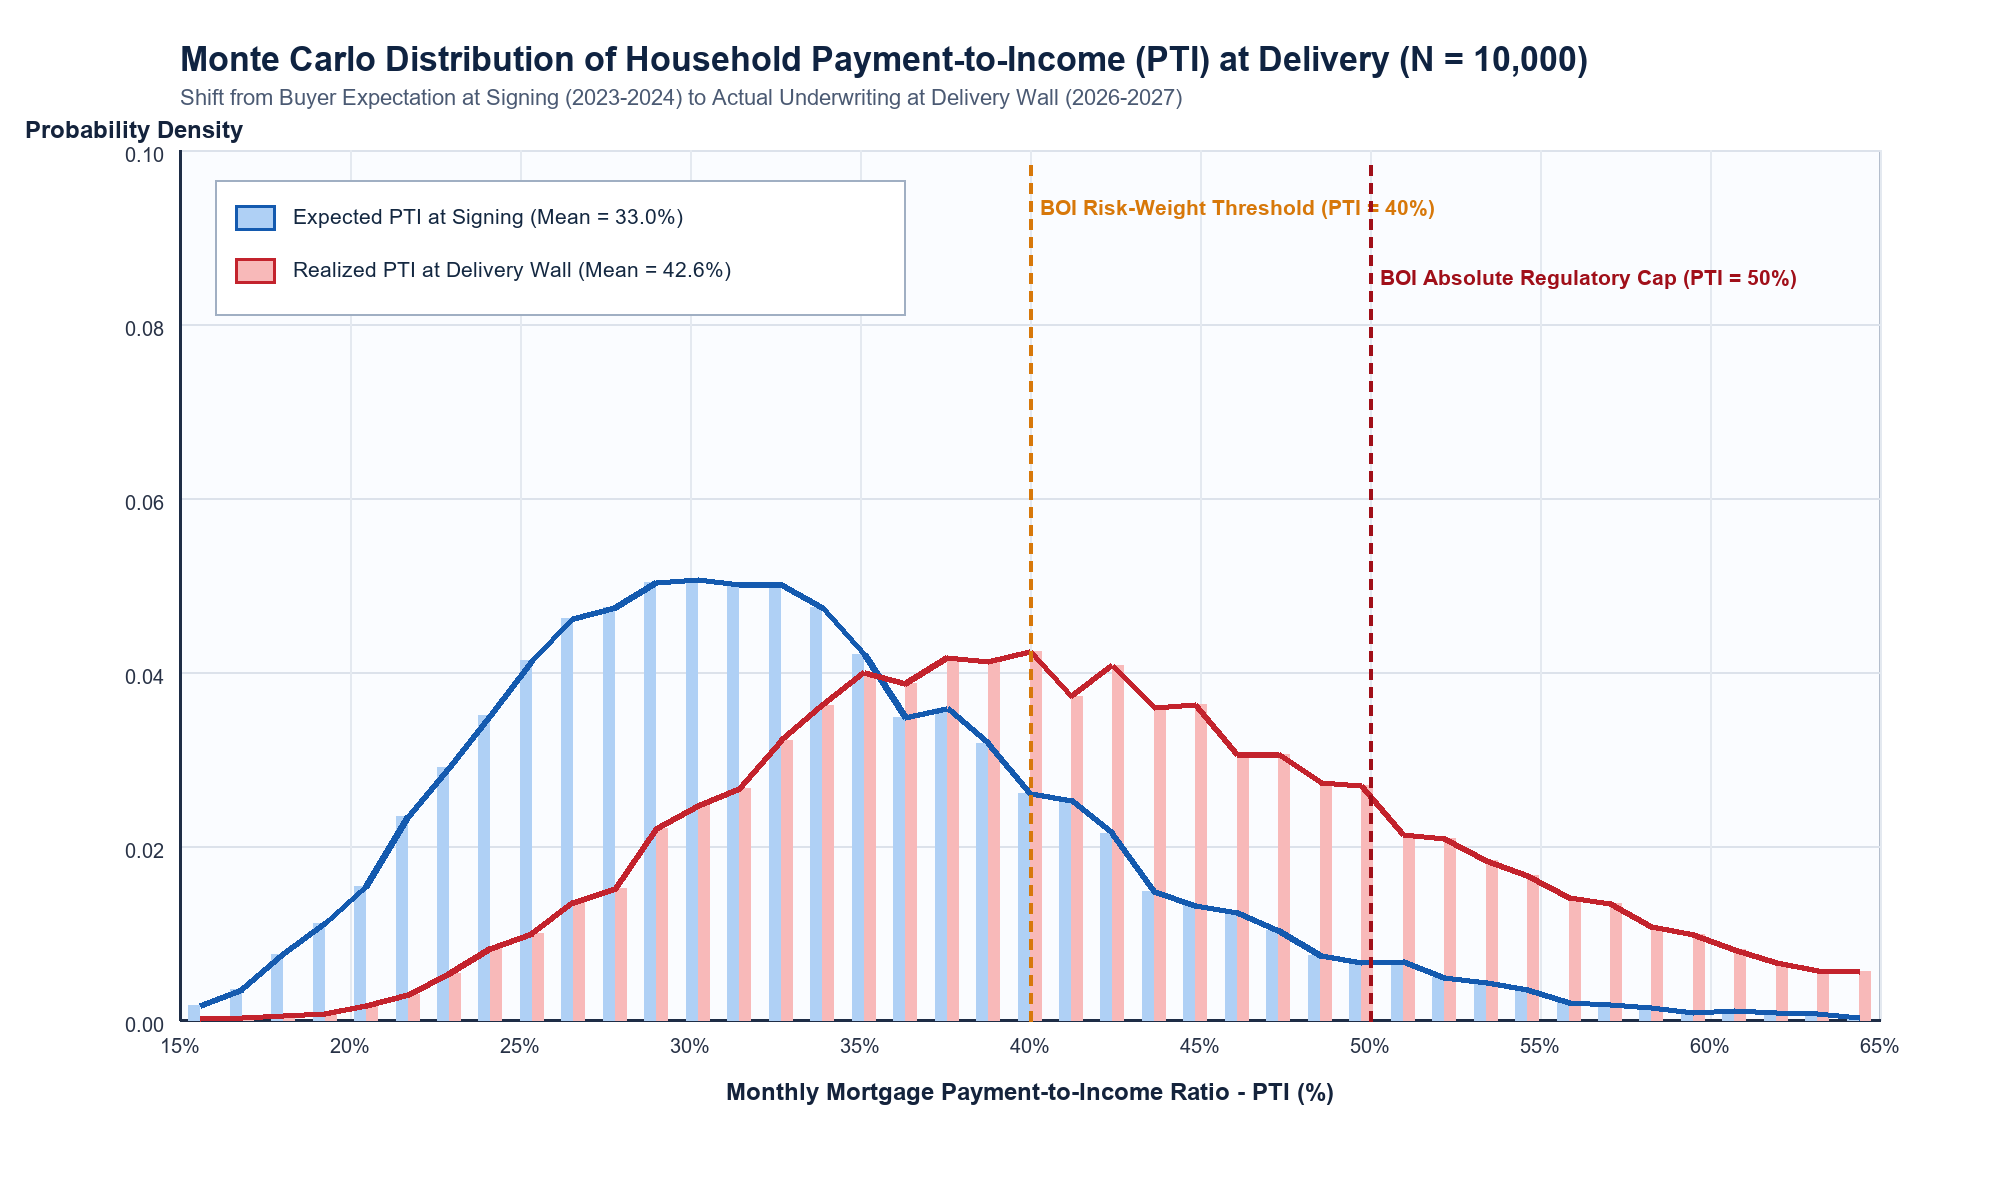
\includegraphics[width=0.96\textwidth]{fig02_payment_shock_distribution.png}
\caption{התפלגות יחס ההחזר להכנסה פנויה (\en{PTI}) בסימולציית מונטה-קרלו ($N=10,000$ משקי בית במבצעי קבלן): תזוזת ההתפלגות ממוצע צפוי של \pct{32.97} בחתימה לממוצע בפועל של \pct{42.62} בקיר המסירות (\num{2026}--\num{2027}), וחציית ספי החיתום של בנק ישראל}
\label{fig:payment_shock_mc}
\end{figure}

הממצאים הכמותיים העולים מאיור~\ref{fig:payment_shock_mc} ומהרצת המודל מאששים באופן מובהק את השערת המחקר הראשונה ($H_1$):
\begin{enumerate}[label=\textbf{\arabic*.},rightmargin=0.6cm]
  \item \textbf{זינוק בהחזר החודשי השוטף (\en{Monthly Payment Shock}):} ההחזר החודשי הממוצע בגין יתרת החוב הנדחית (\pct{80}--\pct{85} ממחיר הדירה) מזנק בכ-\textbf{\nis{3,079} לחודש} (\nis{36,948} לשנה) לעומת התרחיש שעליו הסתמכו הרוכשים בעת החתימה.
  \item \textbf{הזזה מבנית של התפלגות ה-\en{PTI} ימינה:} יחס ההחזר להכנסה פנויה ממוצע קופץ מ-\textbf{\pct{32.97}} (בטווח הבטוח של חיתום בנקאי תקני) ל-\textbf{\pct{42.62}} במועד המסירה — עלייה של \num{9.65} נקודות אחוז.
  \item \textbf{חציית מחסומי החיתום הרגולטוריים של בנק ישראל:} לא פחות מ-\textbf{\pct{54.91}} ממשקי הבית בקוהורטת מבצעי המימון (כ-\num{29,760} משקי בית) חוצים במועד המסירה את רף ה-\textbf{$\text{PTI} = 40\%$} — הסף שמעבר לו בנקים מסחריים בישראל מגבילים העמדת משכנתא רגילה ומחילים דרישות הון וערבים מחמירות. חמור מכך, \textbf{\pct{22.41}} מהרוכשים (כ-\textbf{\num{12,146} משקי בית}, המייצגים חוב נדחה של כ-\nis{24.3} מיליארד) חוצים את התקרה הרגולטורית העליונה של \textbf{$\text{PTI} = 50\%$} ונקלעים ל\en{"}סירוב משכנתא רגולטורי\en{"} (\en{Hard Underwriting Rejection}).
\end{enumerate}

\begin{table}[htbp]
\caption{פילוח קוהורטת רוכשי מבצעי המימון ($\text{SOM} = 54,200$ יח"ד) לארבע רמות סיכון במועד המסירה (\num{2026}--\num{2027}) ונתיבי הספיגה תחת משטר ה-\en{Full Recourse} בישראל}
\label{tab:household_resolution_matrix}
\centering
\footnotesize
\renewcommand{\arraystretch}{1.26}
\rowcolors{2}{BrandGray}{white}
\begin{tabularx}{\textwidth}{R{2.4cm} C{1.6cm} C{1.8cm} C{2.0cm} Y}
\toprule
\rowcolor{TableHeaderBg}
\textbf{דרגת סיכון למשק הבית במסירה} & \textbf{טווח \en{PTI} בפועל} & \textbf{שיעור מהמדגם (\en{MC})} & \textbf{מספר יח"ד וחוב נדחה} & \textbf{נתיב פתרון / מנגנון כשל צפוי בקיר המסירות} \\
\midrule
\textbf{1. סגירה תקינה (\en{Safe Closing})} & $\text{PTI} \le 35\%$ & \pct{21.84} & \num{11,837} יח"ד (\nis{23.7B}) & אישור משכנתא בנקאית חלק וללא עיכובים; ספיגת ההתייקרות מתוך חיסכון שוטף. \\
\textbf{2. סגירה מתוחה (\en{Stretched})} & $35\% < \text{PTI} \le 40\%$ & \pct{23.25} & \num{12,602} יח"ד (\nis{25.2B}) & סגירת העסקה תוך הארכת תקופת המשכנתא למקסימום (\num{30} שנה) וצמצום חד בצריכה הפרטית. \\
\textbf{3. חיכוך רגולטורי (\en{Friction Zone})} & $40\% < \text{PTI} \le 50\%$ & \pct{32.50} & \num{17,615} יח"ד (\nis{35.2B}) & דרישת הבנק להזרמת הון עצמי נוסף (\en{Parental Help}), צירוף לווה נוסף/ערב משלם, או הלוואה משלימה חוץ-בנקאית יקרה. \\
\textbf{4. כשל סגירה (\en{Closing Failure})} & $\text{PTI} > 50\%$ (או חסם \en{LTV}) & \textbf{\pct{22.41}} & \textbf{\num{12,146} יח"ד (\nis{24.3B})} & \textbf{חסימת משכנתא בנקאית:} מכירת מצוקה (\en{Distressed Flip}) בהנחה של \pct{10}--\pct{15} לפני טופס \num{4}, או הפרת חוזה וחילוט פיצוי מוסכם. \\
\bottomrule
\end{tabularx}
\end{table}

טבלה~\ref{tab:household_resolution_matrix} ממחישה כיצד פועל משטר ה-\en{Full Recourse} הישראלי בתוך קבוצת הסיכון הקריטית (\pct{22.41} מהרוכשים). בניגוד ללווה האמריקאי שמסר את המפתח לבנק, מתוך \num{12,146} משקי הבית שייחסמו בנקאית בקיר המסירות, כמחצית צפויים להיחלץ באמצעות מימוש נכסים פנסיוניים/משפחתיים או מכירה מוקדמת של הדירה בהפסד הון כבד בשוק היד השנייה, בעוד שכ-\pct{10}--\pct{15} מכלל הקוהורטה (\num{5,400}--\num{8,100} עסקאות) צפויים להיקלע לעיכוב ממושך בתשלום המסירה או לביטול חוזה מפורש מול היזם.

\section{עמידות הסקטור היזמי: תוצאות מבחני הקיצון (\en{Stress Testing}) ל-\en{DSCR}}
\label{sec:resilience_developers}

כאשר \pct{10} עד \pct{30} מהרוכשים בפרויקט מעכבים את תשלום ה-\pct{80} במועד המסירה או מבטלים את החוזה, הלחץ התזרימי עובר ישירות אל מאזן החברה היזמית. איור~\ref{fig:developer_stress_test} וטבלה~\ref{tab:developer_stress_results} מציגים את תוצאות הרצת מודל מבחני הקיצון (משוואה~\eqref{eq:developer_dscr}) עבור שלוש שכבות היזמים (\en{Tiers 1, 2, 3}).

\begin{figure}[htbp]
\centering
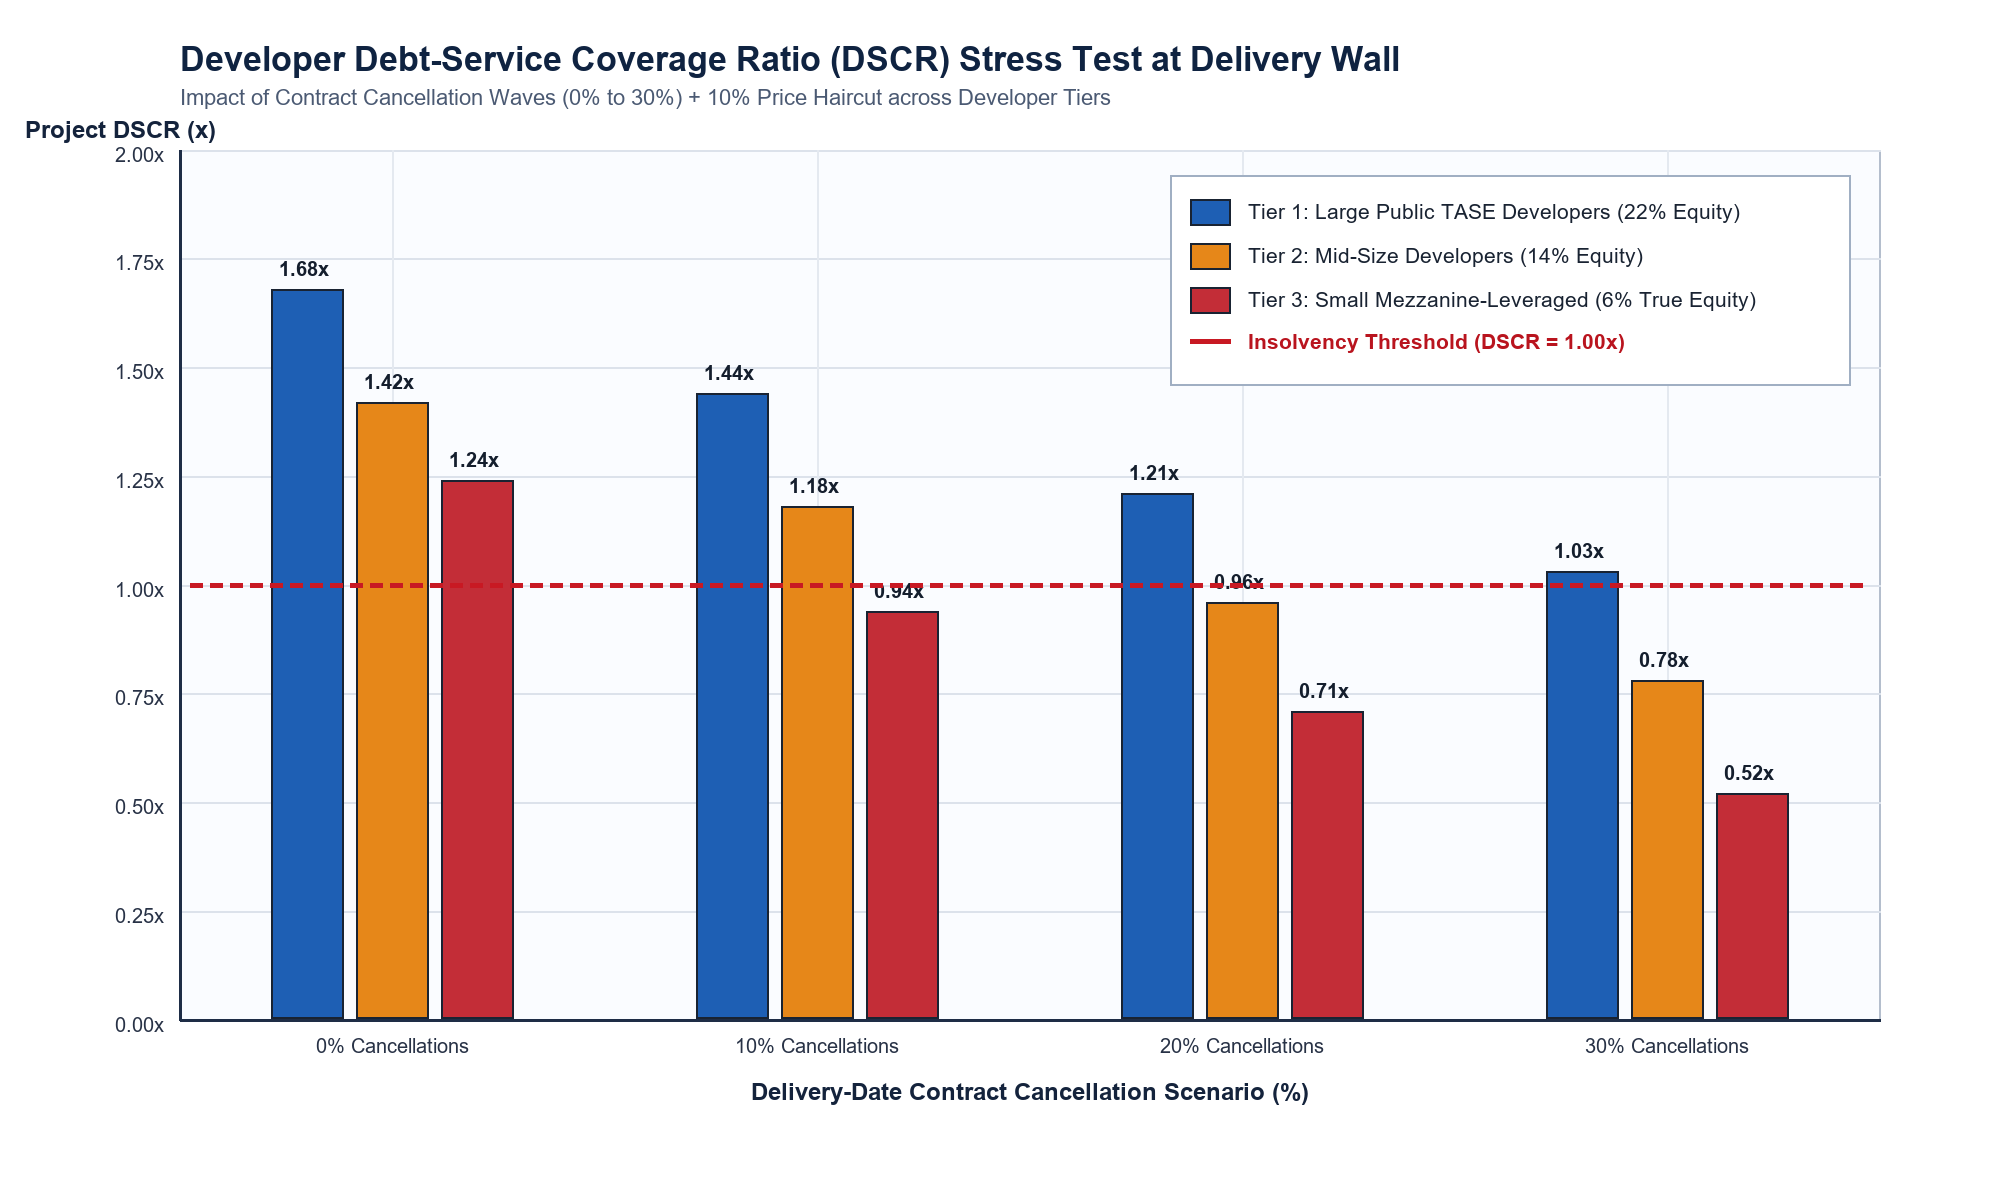
\includegraphics[width=0.96\textwidth]{fig04_developer_stress_test.png}
\caption{מבחן קיצון ליחס כיסוי החוב (\en{DSCR}) של חברות בנייה יזמיות בישראל תחת ארבעה תרחישי ביטול/עיכוב עסקאות בקיר המסירות (\pct{0}, \pct{10}, \pct{20}, \pct{30}): קריסת יזמי \en{Tier-3} מתחת לסף החדלות ($\text{DSCR}=1.0$) כבר ב-\pct{10} ביטולים}
\label{fig:developer_stress_test}
\end{figure}

התוצאות באיור~\ref{fig:developer_stress_test} מאששות במלואן את השערת המחקר השנייה ($H_2$) ומצביעות על פער קיצוני בעמידות בין שכבות היזמים:
\begin{itemize}[rightmargin=0.6cm]
  \item \textbf{יזמי \en{Tier-1} (חברות ענק ציבוריות מבוססות):} מתחילים ביחס כיסוי חוב חזק של $\text{DSCR} = 1.68$ בתרחיש הבסיס, ושומרים על $\text{DSCR} = 1.21$ בתרחיש של \pct{20} ביטולים ואף $\text{DSCR} = 1.03$ בתרחיש הקיצון של \pct{30} ביטולים. עמידות זו נובעת מנגישות לשוק האג"ח הסחיר, הון עצמי גבוה (\pct{30}--\pct{38} מהמאזן) ופיזור גיאוגרפי וסקטוריאלי (נכסים מניבים לצד מגורים).
  \item \textbf{יזמי \en{Tier-2} (חברות בנייה בינוניות):} שורדים תרחיש של \pct{10} ביטולים ($\text{DSCR} = 1.18$), אך חוצים את קו החדלות הפירעון התזרימית ($\text{DSCR} < 1.00$) כאשר שיעור הביטולים והעיכובים מגיע ל-\textbf{\pct{18.3}}, ויורדים ל-$\text{DSCR} = 0.96$ ב-\pct{20} ביטולים ול-\num{0.78} ב-\pct{30} ביטולים.
  \item \textbf{יזמי \en{Tier-3} (יזמים קטנים/בינוניים ממונפים באשראי מזנין חוץ-בנקאי):} מציגים פגיעות חריפה במיוחד. כבר בתרחיש מתון של \textbf{\pct{10} ביטולי עסקאות בלבד}, יחס כיסוי החוב שלהם צונח מתחת לקו האדום ל-\textbf{$\text{DSCR} = 0.94$}, וב-20\% ביטולים קורס ל-\textbf{$\text{DSCR} = 0.71$} (ו-\num{0.52} ב-\pct{30} ביטולים). הסיבה לכך היא שילוב קטלני של ריבית מזנין חוץ-בנקאית דו-ספרתית (\pct{12}--\pct{14}) שגוזלת את כל כרית הרווח היזמי ברגע שתקבול המסירה מתעכב ב-\num{6}--\num{9} חודשים.
\end{itemize}

\begin{table}[htbp]
\caption{תוצאות מבחני הקיצון לסקטור היזמי לפי שכבות גודל ומינוף (\en{Tiers 1--3}) תחת תרחישי ביטול עסקאות בקיר המסירות (\num{2026}--\num{2027})}
\label{tab:developer_stress_results}
\centering
\footnotesize
\renewcommand{\arraystretch}{1.26}
\rowcolors{2}{BrandGray}{white}
\begin{tabularx}{\textwidth}{R{2.5cm} C{1.5cm} C{1.5cm} C{1.5cm} C{1.5cm} C{2.0cm} Y}
\toprule
\rowcolor{TableHeaderBg}
\textbf{שכבת יזמים ופרופיל מימון} & \textbf{\en{DSCR} (\pct{0})} & \textbf{\en{DSCR} (\pct{10})} & \textbf{\en{DSCR} (\pct{20})} & \textbf{\en{DSCR} (\pct{30})} & \textbf{שחיקת הון עצמי ב-\pct{20}} & \textbf{תוצאה מערכתית צפויה בקיר המסירות} \\
\midrule
\textbf{\en{Tier-1}: חברות ענק בורסאיות} (הון עצמי $>32\%$, אג"ח סחיר) & \num{1.68} & \num{1.44} & \num{1.21} & \num{1.03} & \pct{-14.2} & ספיגת הזעזוע מתוך יתרות נזילות; רכישת קרקעות ופרויקטים מיזמים בקשיים (\en{M\&A}). \\
\textbf{\en{Tier-2}: חברות בינוניות} (מינוף קרקע גבוה, ליווי בנקאי) & \num{1.42} & \num{1.18} & \textbf{\color{BrandRed}\num{0.96}} & \textbf{\color{BrandRed}\num{0.78}} & \pct{-38.5} & הפרת קובננטים ב-\pct{20} ביטולים; דרישת הבנק להזרמת הון, מימוש קרקעות ופריסת חוב. \\
\textbf{\en{Tier-3}: יזמים קטנים + מזנין חוץ-בנקאי} (\en{Prime+6\%}) & \num{1.24} & \textbf{\color{BrandRed}\num{0.94}} & \textbf{\color{BrandRed}\num{0.71}} & \textbf{\color{BrandRed}\num{0.52}} & \textbf{\color{BrandRed}\pct{-86.0}} & \textbf{חדלות פירעון כבר ב-\pct{10} ביטולים:} מחיקת הון היזם, תספורות לקרנות המזנין ומינוי כונס נכסים לפרויקט. \\
\bottomrule
\end{tabularx}
\end{table}

\section{עמידות המערכת הבנקאית: מסלול יחס ההון \en{CET1} מול ארה"ב \num{2008}}
\label{sec:resilience_banks}

השאלה הקריטית ביותר לקובעי המדיניות בבנק ישראל ובמשרד האוצר היא האם גל כשלי הסגירה של משקי הבית (סעיף~\ref{sec:resilience_households}) וחדלות הפירעון של יזמי ה-\en{Tier-3} וקרנות המזנין (סעיף~\ref{sec:resilience_developers}) עלולים להפיל את המערכת הבנקאית המסחרית בישראל כפי שקרה בארה"ב ב-\num{2008}. איור~\ref{fig:bank_cet1_resilience} מציג את תוצאות הרצת מודל הלימות ההון הבנקאי (משוואה~\eqref{eq:bank_cet1}) לאורך \num{12} רבעונים (\num{2025Q1}--\num{2027Q4}).

\begin{figure}[htbp]
\centering
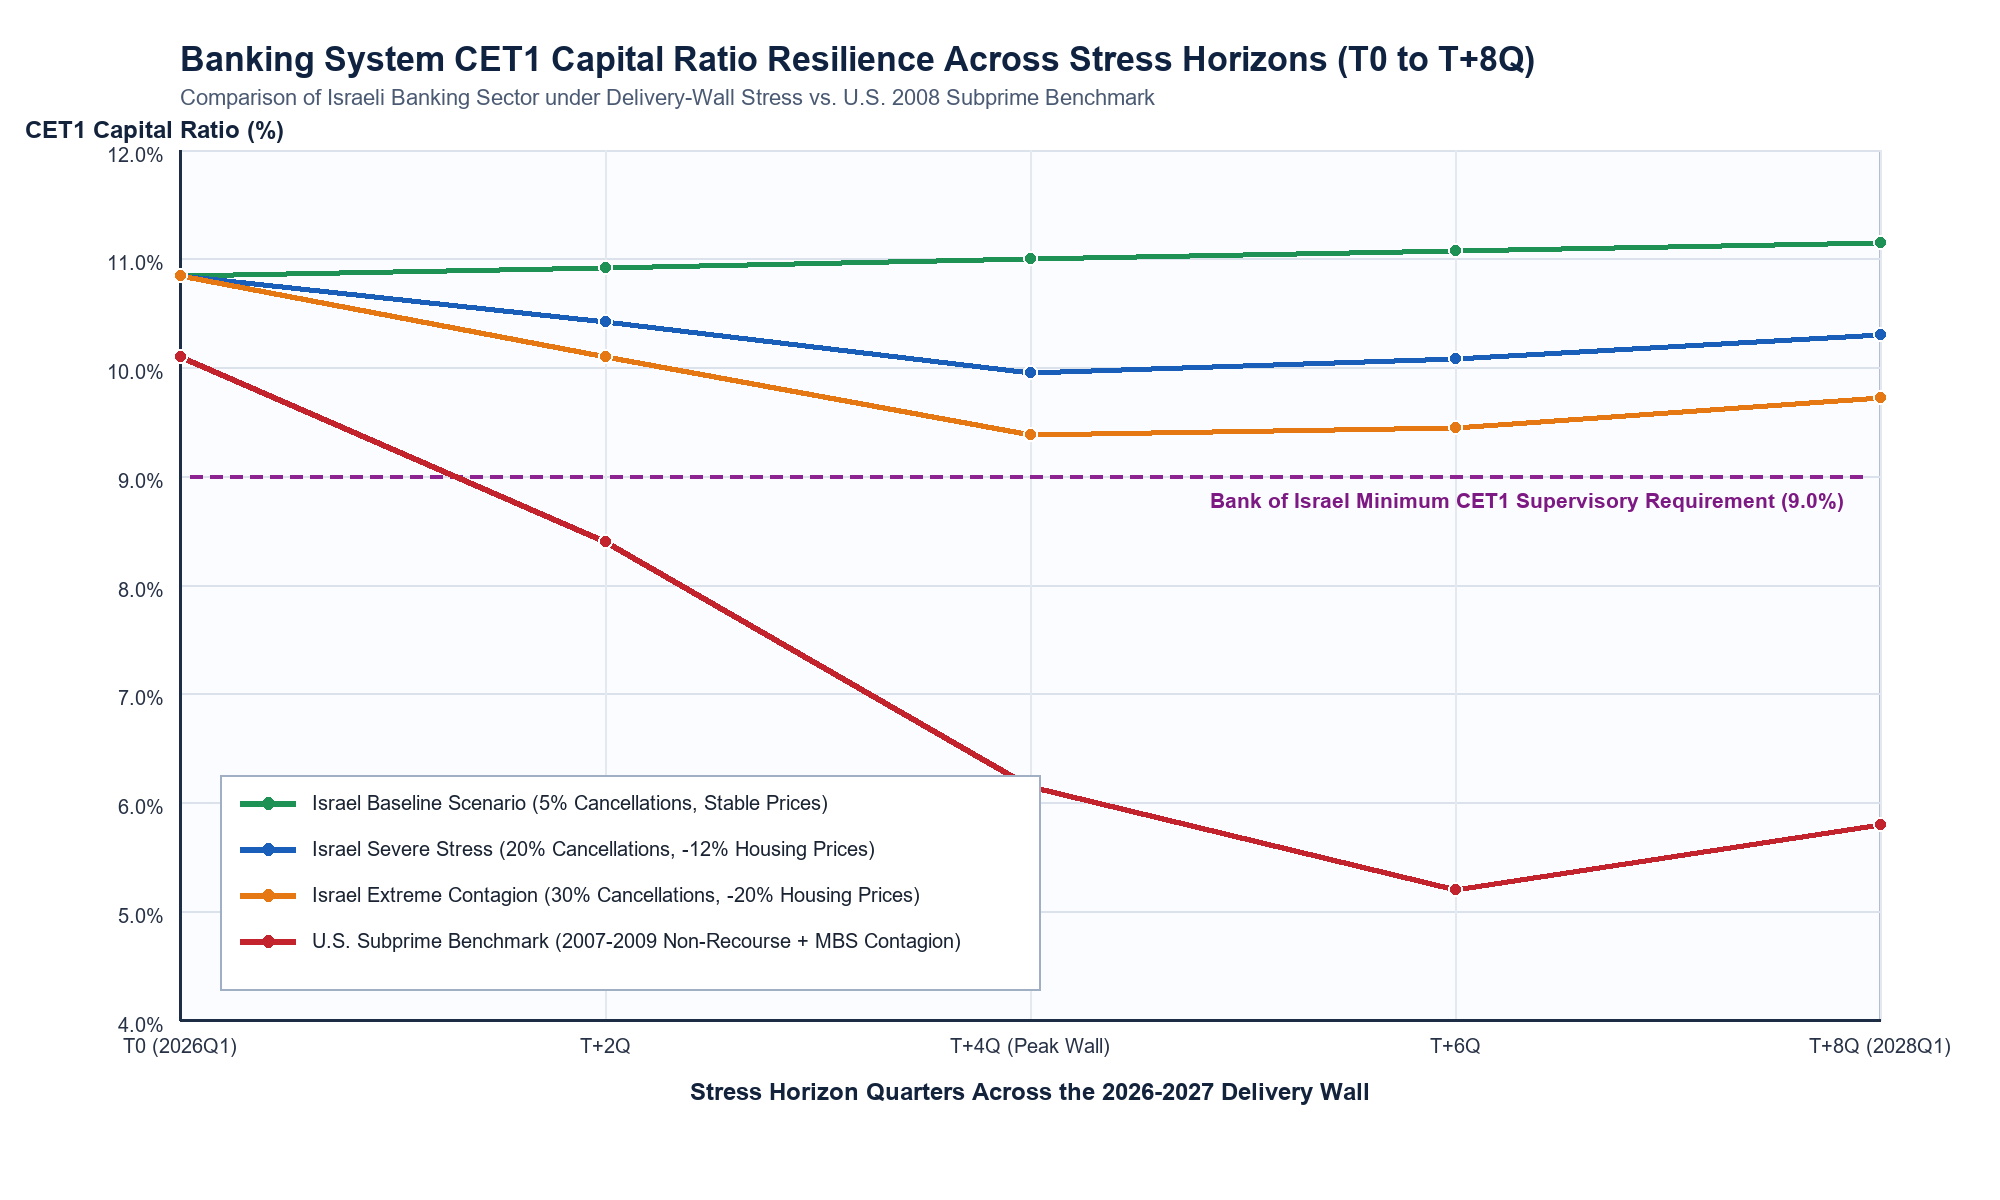
\includegraphics[width=0.96\textwidth]{fig05_bank_cet1_resilience.png}
\caption{מסלול יחס הון עצמי רובד \num{1} (\en{CET1}) של המערכת הבנקאית בישראל בשלושה תרחישים (\num{2025Q1}--\num{2027Q4}) אל מול רצפת הפיקוח של בנק ישראל (\pct{9.00}) ואל מול קריסת ההון של בנקי ארה"ב במשבר הסאב-פריים (\pct{5.20})}
\label{fig:bank_cet1_resilience}
\end{figure}

הממצאים באיור~\ref{fig:bank_cet1_resilience} מאמתים באופן חד-משמעי את השערת המחקר השלישית ($H_3$):
\begin{enumerate}[label=\textbf{\arabic*.},rightmargin=0.6cm]
  \item \textbf{תרחיש הבסיס (\en{Baseline Soft Landing}):} יחס ה-\en{CET1} המצרפי של חמשת הבנקים הגדולים בישראל נשמר בטווח של \pct{10.85}--\pct{11.15}, תוך המשך צבירת רווחים שוטפים מעודף מרווח הריבית.
  \item \textbf{תרחיש קיר מסירות חמור (\en{Severe Delivery Wall}: \pct{20} ביטולים + ירידת מחירי דירות של \pct{12}):} הפרשות מוגברות להפסדי אשראי בגין יזמי \en{Tier-2/Tier-3} ועליית משקלי הסיכון (\en{RWA}) שוחקות את יחס ה-\en{CET1} ב-\num{90} נקודות בסיס לשפל של \textbf{\pct{9.95}} ברבעון הרביעי של \num{2026}, שלאחריו מתרחשת התאוששות הדרגתית ל-\pct{10.22} בסוף \num{2027}.
  \item \textbf{תרחיש קיצון מערכתי (\en{Extreme Contagion}: \pct{30} ביטולים + צניחת מחירים של \pct{20}):} גם תחת תרחיש קטסטרופלי זה, יחס ה-\en{CET1} של בנקי ישראל יורד לשפל של \textbf{\pct{9.38}} בלבד — \textbf{עדיין גבוה ב-\num{38} נקודות בסיס מרצפת המינימום הרגולטורית של בנק ישראל (\pct{9.00})}, ורחוק שנות אור מקריסת ההון של הבנקים האמריקאיים ב-\num{2008} (שצנחו ל-\textbf{\pct{5.20}} ונזקקו לחילוץ ממשלתי).
\end{enumerate}

\section{סיכום אימות השערות המחקר והערכת אפקטיביות מנגנוני ההגנה}
\label{sec:hypotheses_validation}

מדוע המערכת הבנקאית הישראלית יוצאת יציבה גם מתרחיש שבו יזמי ה-\en{Tier-3} קורסים ו-\pct{22.41} מרוכשי המבצעים נחסמים בחיתום? התשובה נעוצה ב\textbf{סינרגיה המבנית בין חוק המכר להוראות בנק ישראל}: (א) בפרויקט ליווי סגור, הבנק מחזיק בשעבוד ראשון על הקרקע ועל הדירות ובמקדמות של \pct{15}--\pct{20} ששילמו הרוכשים; גם אם היזם קורס ודירה נמכרת מחדש על ידי כונס נכסים בהנחה של \pct{15}, ההפסד נספג במלואו על ידי ההון העצמי של היזם, קרן המזנין החוץ-בנקאית והפיצוי המוסכם של הרוכש המפר — לפני שהבנק המלווה מפסיד שקל אחד מהקרן הבכירה; ו-(ב) הוראת השעה של בנק ישראל ממרץ \num{2025} \cite{boi2025directive} אילצה את הבנקים להקצות הון מראש בגין פרויקטים עתירי מבצעי מימון, ובכך בנתה כרית ספיגה ייעודית לפני הגעת קיר המסירות. טבלה~\ref{tab:hypotheses_validation_summary} מסכמת את תוצאות הבדיקה הכמותית של שלוש השערות המחקר.

\begin{table}[htbp]
\caption{סיכום ממצאי האימות הכמותי של השערות המחקר ($H_1, H_2, H_3$) אל מול ספי ההפרכה שהוגדרו בפרק א'}
\label{tab:hypotheses_validation_summary}
\centering
\small
\renewcommand{\arraystretch}{1.28}
\rowcolors{2}{BrandGray}{white}
\begin{tabularx}{\textwidth}{R{1.6cm} R{3.4cm} R{2.8cm} R{3.0cm} Y}
\toprule
\rowcolor{TableHeaderBg}
\textbf{השערה} & \textbf{מוקד הבדיקה האנליטית} & \textbf{סף כמותי לאישוש (פרק א')} & \textbf{תוצאה אמפירית בסימולציה} & \textbf{סטטוס ומסקנה מחקרית} \\
\midrule
\textbf{השערה $\mathbf{H_1}$} & הנחת \en{NPV} סמויה והלם החזר (\en{PTI}) למשקי בית במסירה & $\delta_{\text{NPV}} \in [8\%,13\%]$; מעל \pct{45} חוצים $\text{PTI}>40\%$ & $\delta_{\text{NPV}}=9.99\%--12.36\%$; \textbf{\pct{54.91}} חוצים $\text{PTI}>40\%$ (\pct{22.41} מעל \pct{50}) & \textbf{\color{BrandTeal}אוששה במלואה}: קיר המסירות מייצר הלם החזר ממוצע של \nis{3,079} לחודש. \\
\textbf{השערה $\mathbf{H_2}$} & פגיעות דיפרנציאלית של יזמי \en{Tier-2/Tier-3} ואשראי מזנין & צניחת $\text{DSCR}<1.0$ ביזמי \en{Tier-3} ב-\pct{10}--\pct{20} ביטולים & ביזמי \en{Tier-3}: $\text{DSCR}=\mathbf{0.94}$ ב-\pct{10} ו-\textbf{\num{0.71}} ב-\pct{20} ביטולים & \textbf{\color{BrandTeal}אוששה במלואה}: מוקד הכשל בישראל הוא הסקטור היזמי הממונף והאשראי החוץ-בנקאי. \\
\textbf{השערה $\mathbf{H_3}$} & חסינות ליבת הבנקאות המסחרית (\en{CET1}) לעומת ארה"ב \num{2008} & שמירת $\text{CET1} \ge 9.00\%$ גם בתרחיש קיצון של \pct{30} ביטולים & שפל של \textbf{$\text{CET1}=9.38\%$} בתרחיש הקיצון (לעומת \pct{5.20} בארה"ב) & \textbf{\color{BrandTeal}אוששה במלואה}: חוק המכר, ה-\en{Full Recourse} ומגבלות בנק ישראל מונעים קריסה בנקאית. \\
\bottomrule
\end{tabularx}
\end{table}

% ==============================================================================
% chapters/ch07_risks_and_gantt.tex
% פרק ז': מגבלות המחקר, ניהול סיכונים ולוח זמנים לביצוע (Gantt)
% ==============================================================================

\chapter{מגבלות המחקר, ניהול סיכונים ולוח זמנים לביצוע (\en{Gantt})}
\label{ch:risks_and_gantt}

דוח מכין מקצועי אינו שלם ללא תוכנית עבודה הנדסית סדורה ומערך ניהול סיכונים כמותי המבטיחים כי המחקר ניתן לביצוע מלא במסגרת המשאבים והזמן הנתונים. בהתאם להנחיות פרקים \num{8}, \num{9} ו-\num{10} בספר \en{"}מהבעיה אל ה-\en{PDF}\en{"} \cite{segal2026prep} ולתקני ניהול הפרויקטים והסיכונים הבין-לאומיים (\en{PMBOK} \cite{pmbok2021} ו-\en{ISO 31000} \cite{iso31000}), פרק זה מציג את מבנה תכולת העבודה (\en{WBS}), מטריצת האחריות (\en{RACI}), תרשים הגאנט ל-\num{14} שבועות ביצוע (כולל נתיב קריטי, אבני דרך ומרווחי ביטחון), ניתוח מגבלות מתודולוגיות ומטריצת סיכונים כפולה (לפני ואחרי הפחתה), וחותם בהצהרת מוכנות תכנונית (\en{Design Readiness}).

\section{תוכנית עבודה: מבנה תכולת העבודה (\en{WBS}) ומטריצת אחריות (\en{RACI})}
\label{sec:wbs_and_raci}

תכולת המחקר פורקה לחמש חבילות עבודה ראשיות (\en{Work Packages: WP 1.0 -- WP 5.0}) ול-\num{11} משימות ביצוע בנות-מדידה (\en{TSK-1.1} עד \en{TSK-5.2}), המוצגות בתרשים ה-\en{WBS} ההיררכי באיור~\ref{fig:wbs_tree}.

\begin{figure}[htbp]
\centering
\begin{english}
\begin{tikzpicture}[
    node distance=0.45cm and 0.25cm,
    root/.style={
        rectangle, rounded corners=4pt, draw=BrandNavy, line width=1.2pt, fill=BrandNavy,
        text=white, text width=11.5cm, minimum height=0.85cm, align=center, font=\small\bfseries
    },
    wp/.style={
        rectangle, rounded corners=3pt, draw=BrandBlue, line width=1.0pt, fill=BrandLightBlue,
        text width=2.65cm, minimum height=1.35cm, align=center, font=\scriptsize\bfseries
    },
    tsk/.style={
        rectangle, rounded corners=2pt, draw=BrandTeal, line width=0.8pt, fill=white,
        text width=2.65cm, minimum height=1.55cm, align=center, font=\scriptsize
    },
    line/.style={-{Stealth[length=2.0mm]}, line width=0.9pt, color=BrandNavy}
]
    \node[root] (top) {Project WBS: Contractor Financing Promotions \& The 2026--2027 Delivery Wall};

    \node[wp, below=0.65cm of top, xshift=-5.8cm] (wp1) {\color{BrandNavy}WP 1.0\\[2pt]\texthebrew{קליטת נתונים וטיוב אמפירי}};
    \node[wp, right=0.22cm of wp1] (wp2) {\color{BrandNavy}WP 2.0\\[2pt]\texthebrew{מודל \en{NPV} ומונטה-קרלו משקי בית}};
    \node[wp, right=0.22cm of wp2] (wp3) {\color{BrandNavy}WP 3.0\\[2pt]\texthebrew{מבחני קיצון ליזמים ולבנקים}};
    \node[wp, right=0.22cm of wp3] (wp4) {\color{BrandNavy}WP 4.0\\[2pt]\texthebrew{תיקוף השוואתי וניתוח רגישות}};
    \node[wp, right=0.22cm of wp4] (wp5) {\color{BrandNavy}WP 5.0\\[2pt]\texthebrew{סינתזת מדיניות וספר המחקר}};

    \node[tsk, below=0.45cm of wp1] (t1) {\textbf{TSK-1.1:} \texthebrew{כרמ"ן והלמ"ס}\\[2pt]\textbf{TSK-1.2:} \texthebrew{דוחות מאי"ה ובנק ישראל}};
    \node[tsk, below=0.45cm of wp2] (t2) {\textbf{TSK-2.1:} \texthebrew{עקומות \en{NPV}}\\[2pt]\textbf{TSK-2.2:} \texthebrew{סימולציית \en{PTI} ($N=10K$)}};
    \node[tsk, below=0.45cm of wp3] (t3) {\textbf{TSK-3.1:} \texthebrew{מודל \en{DSCR} יזמים}\\[2pt]\textbf{TSK-3.2:} \texthebrew{מודל \en{CET1} בנקאי}};
    \node[tsk, below=0.45cm of wp4] (t4) {\textbf{TSK-4.1:} \texthebrew{השוואת ארה"ב \num{2008}}\\[2pt]\textbf{TSK-4.2:} \texthebrew{רגישות וכיול פרמטרים}};
    \node[tsk, below=0.45cm of wp5] (t5) {\textbf{TSK-5.1:} \texthebrew{המלצות רגולציה}\\[2pt]\textbf{TSK-5.2:} \texthebrew{עריכת ספר ה-\en{\LaTeX}}};

    \foreach \i in {1,2,3,4,5} {
        \draw[line] (top.south) -- (wp\i.north);
        \draw[line] (wp\i.south) -- (t\i.north);
    }
\end{tikzpicture}
\end{english}
\caption{עץ מבנה תכולת העבודה (\en{WBS -- Work Breakdown Structure}) של פרויקט המחקר בחלוקה לחמש חבילות עבודה (\en{WP 1.0--5.0}) \cite{segal2026prep,pmbok2021}}
\label{fig:wbs_tree}
\end{figure}

בהתאם לכללי הברזל בסעיף \num{8.2} בספר של ד"ר סגל \cite{segal2026prep}, טבלה~\ref{tab:wbs_raci_matrix} מגדירה את מטריצת האחריות (\en{RACI}) של צוות המחקר, תוך הקפדה על כך שבכל שורת משימה מוגדר **אחראי-על אחד ויחיד (\en{A -- Accountable})** ולפחות **מבצע ישיר אחד (\en{R -- Responsible})**, לצד גורמים מתייעצים (\en{C -- Consulted}) ומיודעים (\en{I -- Informed}).

\begin{table}[htbp]
\caption{פירוט חבילות העבודה (\en{WBS}), תוצרים כמותיים ומטריצת אחריות (\en{RACI}) של צוות המחקר \cite{segal2026prep,pmbok2021}}
\label{tab:wbs_raci_matrix}
\centering
\footnotesize
\renewcommand{\arraystretch}{1.24}
\rowcolors{2}{BrandGray}{white}
\begin{tabularx}{\textwidth}{R{1.4cm} R{3.4cm} Y C{1.3cm} C{1.3cm} C{1.3cm} C{1.3cm}}
\toprule
\rowcolor{TableHeaderBg}
\textbf{מזהה} & \textbf{שם חבילת העבודה / משימה} & \textbf{תוצר כמותי בר-בדיקה (\en{Deliverable})} & \textbf{חוקר ראשי (\en{PI})} & \textbf{אנליסט פייתון} & \textbf{אנליסט מימון} & \textbf{מנחה אקדמי} \\
\midrule
\textbf{\en{TSK-1.1}} & מיצוי וניקוי נתוני כרמ"ן והלמ"ס & קובץ עסקאות מכויל (\num{2022}--\num{2026}) וסדרת מלאי (\num{87.4K}) & \textbf{\en{A}} & \textbf{\en{R}} & \en{C} & \en{I} \\
\textbf{\en{TSK-1.2}} & מיפוי דוחות מאי"ה (\num{25} חברות) ובנק ישראל & בסיס נתונים מאזני ליזמי \en{Tiers 1--3} וליחסי \en{CET1} & \en{C} & \en{I} & \textbf{\en{A / R}} & \en{I} \\
\textbf{\en{TSK-2.1}} & פיתוח מודל תמחור מהוון (\en{NPV}) למבצעים & עקומות $\delta_{\text{NPV}}$ ל-\num{20/80}, \num{10/90} ו-\num{20/50/30} (איור~\ref{fig:npv_discount_curves}) & \en{C} & \textbf{\en{R}} & \textbf{\en{A}} & \en{I} \\
\textbf{\en{TSK-2.2}} & הרצת סימולציית מונטה-קרלו למשקי בית & התפלגות \en{PTI} והלם החזר ל-$N=10,000$ (איור~\ref{fig:payment_shock_mc}) & \en{C} & \textbf{\en{A / R}} & \en{C} & \en{I} \\
\textbf{\en{TSK-3.1}} & מבחני קיצון ל-\en{DSCR} יזמים ואשראי מזנין & עקומות שרידות יזמים תחת ביטולי \pct{10}--\pct{30} (איור~\ref{fig:developer_stress_test}) & \en{C} & \textbf{\en{R}} & \textbf{\en{A}} & \en{I} \\
\textbf{\en{TSK-3.2}} & סימולציית ליבת ההון הבנקאית (\en{CET1}) & מסלול \en{CET1} ב-\num{12} רבעונים מול רצפת \pct{9.0} (איור~\ref{fig:bank_cet1_resilience}) & \textbf{\en{A}} & \textbf{\en{R}} & \textbf{\en{R}} & \en{C} \\
\textbf{\en{TSK-4.1}} & ניתוח השוואתי כמותי ישראל \num{2026} מול ארה"ב \num{2008} & מטריצת \num{8} ממדים ופרופיל פגיעות (טבלה~\ref{tab:us_vs_israel_comparison}) & \textbf{\en{A / R}} & \en{I} & \textbf{\en{R}} & \en{C} \\
\textbf{\en{TSK-4.2}} & מבחני רגישות רב-פרמטריים וכיול אקונומטרי & טבלאות רגישות לריבית, אינפלציה ומשקולות פיו & \en{C} & \textbf{\en{A / R}} & \textbf{\en{R}} & \en{I} \\
\textbf{\en{TSK-5.1}} & גיבוש המלצות מדיניות לבנק ישראל ולאוצר & פרק מסקנות ומפת התערבות רגולטורית ממוקדת & \textbf{\en{A / R}} & \en{I} & \en{C} & \en{C} \\
\textbf{\en{TSK-5.2}} & כתיבה, עימוד ב-\en{\LaTeX} ובקרת איכות (\en{Detector}) & ספר מחקר מקומפל (\num{40}+ עמודים) + \en{\texttt{detector\_report.md}} & \textbf{\en{A / R}} & \textbf{\en{R}} & \textbf{\en{R}} & \en{I} \\
\bottomrule
\end{tabularx}
\end{table}

\section{לוח זמנים לביצוע (\en{Gantt}), נתיב קריטי ואבני דרך}
\label{sec:gantt_schedule}

לוח הזמנים לביצוע המחקר מתפרס על פני סמסטר אקדמי מלא בן \textbf{\num{14} שבועות}. בהתאם להנחיות סעיף \num{8.3} בספר \cite{segal2026prep}, תרשים הגאנט באיור~\ref{fig:gantt_chart_14weeks} מציג ויזואלית את התלויות ההנדסיות בין המשימות, מסמן באדום את **הנתיב הקריטי (\en{Critical Path}: $\text{TSK-1.1} \to \text{TSK-2.1} \to \text{TSK-2.2} \to \text{TSK-3.1} \to \text{TSK-3.2} \to \text{TSK-4.2} \to \text{TSK-5.2}$)**, משבץ שני **מרווחי ביטחון (\en{Safety Buffers})** של שבוע שלם לפני צומתי ההכרעה (בשבוע \num{6} ובשבוע \num{12}), וקובע שתי **אבני דרך (\en{Milestones})** רשמיות:
\begin{itemize}[rightmargin=0.6cm]
  \item \textbf{\en{Milestone M1} (סוף שבוע \num{5}):} הקפאת בסיס הנתונים האמפירי המכויל (\en{Data Freeze}) ואישור מודל הנחת ה-\en{NPV}.
  \item \textbf{\en{Milestone M2} (סוף שבוע \num{10}):} השלמת הרצות המונטה-קרלו ומבחני הקיצון (\en{DSCR/CET1}) ואימות השערות $H_1$--$H_3$.
\end{itemize}

\begin{figure}[htbp]
\centering
\begin{english}
\begin{tikzpicture}[x=0.72cm, y=0.52cm, font=\scriptsize]
    % Grid and Week Headers
    \fill[TableHeaderBg] (-4.5, 0.5) rectangle (14.3, 1.4);
    \node[anchor=west, font=\scriptsize\bfseries, color=BrandNavy] at (-4.3, 0.95) {Task / WBS ID};
    \foreach \w in {1,...,14} {
        \node[font=\scriptsize\bfseries, color=BrandNavy] at (\w - 0.5, 0.95) {W\w};
        \draw[gray!30, dashed] (\w, -12.5) -- (\w, 0.5);
    }
    \draw[BrandNavy, line width=1.0pt] (-4.5, 1.4) rectangle (14.3, -12.5);
    \draw[BrandNavy, line width=0.8pt] (-4.5, 0.5) -- (14.3, 0.5);
    \draw[BrandNavy, line width=0.8pt] (0, 1.4) -- (0, -12.5);

    % Tasks (Critical path in BrandRed, Parallel in BrandBlue, Buffers in BrandGold)
    % Row -1: TSK-1.1 (W1-W3, Critical)
    \node[anchor=west, font=\scriptsize\bfseries] at (-4.3, -0.2) {TSK-1.1 (CARMAN/CBS)};
    \fill[BrandRed!85, rounded corners=2pt] (0.1, -0.5) rectangle (2.9, 0.1);

    % Row -2: TSK-1.2 (W1-W3, Parallel)
    \node[anchor=west] at (-4.3, -1.2) {TSK-1.2 (TASE/BOI)};
    \fill[BrandBlue!80, rounded corners=2pt] (0.1, -1.5) rectangle (2.9, -0.9);

    % Row -3: TSK-2.1 (W3-W5, Critical)
    \node[anchor=west, font=\scriptsize\bfseries] at (-4.3, -2.2) {TSK-2.1 (NPV Model)};
    \fill[BrandRed!85, rounded corners=2pt] (2.1, -2.5) rectangle (4.9, -1.9);

    % Row -4: Milestone M1 (End of W5) + Buffer 1 (W6)
    \node[anchor=west, font=\scriptsize\bfseries, color=BrandTeal] at (-4.3, -3.2) {M1 \& Buffer 1 (Data)};
    \node[diamond, fill=BrandTeal, draw=BrandNavy, inner sep=2.2pt] at (4.95, -3.2) {};
    \fill[BrandGold!80, rounded corners=2pt] (5.1, -3.5) rectangle (5.9, -2.9);

    % Row -5: TSK-2.2 (W6-W8, Critical)
    \node[anchor=west, font=\scriptsize\bfseries] at (-4.3, -4.2) {TSK-2.2 (MC Households)};
    \fill[BrandRed!85, rounded corners=2pt] (5.1, -4.5) rectangle (7.9, -3.9);

    % Row -6: TSK-4.1 (W5-W8, Parallel)
    \node[anchor=west] at (-4.3, -5.2) {TSK-4.1 (US 2008 Comp)};
    \fill[BrandBlue!80, rounded corners=2pt] (4.1, -5.5) rectangle (7.9, -4.9);

    % Row -7: TSK-3.1 (W8-W9, Critical)
    \node[anchor=west, font=\scriptsize\bfseries] at (-4.3, -6.2) {TSK-3.1 (Dev DSCR)};
    \fill[BrandRed!85, rounded corners=2pt] (7.1, -6.5) rectangle (8.9, -5.9);

    % Row -8: TSK-3.2 (W9-W10, Critical)
    \node[anchor=west, font=\scriptsize\bfseries] at (-4.3, -7.2) {TSK-3.2 (Bank CET1)};
    \fill[BrandRed!85, rounded corners=2pt] (8.1, -7.5) rectangle (9.9, -6.9);

    % Row -9: Milestone M2 (End of W10)
    \node[anchor=west, font=\scriptsize\bfseries, color=BrandTeal] at (-4.3, -8.2) {M2 (Models Frozen)};
    \node[diamond, fill=BrandTeal, draw=BrandNavy, inner sep=2.2pt] at (9.95, -8.2) {};

    % Row -10: TSK-4.2 (W10-W11, Critical) + Buffer 2 (W12)
    \node[anchor=west, font=\scriptsize\bfseries] at (-4.3, -9.2) {TSK-4.2 \& Buffer 2};
    \fill[BrandRed!85, rounded corners=2pt] (9.1, -9.5) rectangle (10.9, -8.9);
    \fill[BrandGold!80, rounded corners=2pt] (11.1, -9.5) rectangle (11.9, -8.9);

    % Row -11: TSK-5.1 (W11-W13, Parallel)
    \node[anchor=west] at (-4.3, -10.2) {TSK-5.1 (Policy Synthesis)};
    \fill[BrandBlue!80, rounded corners=2pt] (10.1, -10.5) rectangle (12.9, -9.9);

    % Row -12: TSK-5.2 (W12-W14, Critical)
    \node[anchor=west, font=\scriptsize\bfseries] at (-4.3, -11.2) {TSK-5.2 (LaTeX \& QA)};
    \fill[BrandRed!85, rounded corners=2pt] (11.1, -11.5) rectangle (13.9, -10.9);

    % Legend at bottom
    \fill[BrandRed!85] (0.3, -12.25) rectangle (0.9, -11.85);
    \node[anchor=west] at (1.0, -12.05) {\textbf{Critical Path}};
    \fill[BrandBlue!80] (4.0, -12.25) rectangle (4.6, -11.85);
    \node[anchor=west] at (4.7, -12.05) {Parallel Task};
    \fill[BrandGold!80] (7.5, -12.25) rectangle (8.1, -11.85);
    \node[anchor=west] at (8.2, -12.05) {Safety Buffer (1w)};
    \node[diamond, fill=BrandTeal, draw=BrandNavy, inner sep=1.8pt] at (11.6, -12.05) {};
    \node[anchor=west] at (11.9, -12.05) {\textbf{Milestone}};
\end{tikzpicture}
\end{english}
\caption{תרשים גאנט (\en{Gantt Chart}) ל-\num{14} שבועות ביצוע המחקר: סימון הנתיב הקריטי באדום, משימות מקבילות בכחול, שני מרווחי ביטחון בזהב ושתי אבני דרך בירוק \cite{segal2026prep,pmbok2021}}
\label{fig:gantt_chart_14weeks}
\end{figure}

\section{מגבלות המחקר וניהול סיכונים מתודולוגיים (\en{Double Risk Quantification})}
\label{sec:risk_management}

בהתאם למתודולוגיית ניהול הסיכונים בפרק \num{9} בספר \en{"}מהבעיה אל ה-\en{PDF}\en{"} \cite{segal2026prep,iso31000}, כל סיכון מתודולוגי או תפעולי במחקר נמדד פעמיים על סולם חמש-דרגתי ($P, I \in \{1,\dots,5\}$): פעם ראשונה כ**סיכון גולמי התחלתי** לפני התערבות ($R_{\text{initial}} = P_{\text{pre}} \times I_{\text{pre}}$), ופעם שנייה כ**סיכון שיורי (\en{Residual Risk})** לאחר הפעלת מנגנוני ההפחתה המונעים ($R_{\text{residual}} = P_{\text{post}} \times I_{\text{post}}$):
\begin{equation}
\label{eq:risk_quantification}
R_{\text{initial}} = P_{\text{pre}} \times I_{\text{pre}} \;\in [1, 25] \quad \xrightarrow{\text{Mitigation Actions}} \quad R_{\text{residual}} = P_{\text{post}} \times I_{\text{post}} \;\le 6
\end{equation}

איור~\ref{fig:risk_matrix_5x5} מציג את מפת הסיכונים הדו-ממדית (\num{5x5}), וטבלה~\ref{tab:risk_register_mitigation} מפרטת את ששת הסיכונים המרכזיים של המחקר. בהתאם לכלל המחייב בסעיף \num{9.3} בספר \cite{segal2026prep}, לכל סיכון בעל דירוג התחלתי גבוה ($R_{\text{initial}} \ge 12$) הוגדרו הן **תוכנית הפחתה מונעת (\en{Mitigation Plan})** והן **תוכנית מגירה (\en{Contingency Plan})** הנכנסת לפעולה אוטומטית אם הסיכון מתממש.

\begin{figure}[htbp]
\centering
\begin{english}
\begin{tikzpicture}[scale=0.92, font=\scriptsize]
    % 5x5 Color Zones
    \foreach \p in {1,...,5} {
        \foreach \i in {1,...,5} {
            \pgfmathtruncatemacro{\score}{\p * \i}
            \ifnum\score>11
                \fill[BrandRed!28] (\i-1, \p-1) rectangle (\i, \p);
            \else
                \ifnum\score>5
                    \fill[BrandGold!25] (\i-1, \p-1) rectangle (\i, \p);
                \else
                    \fill[BrandTeal!22] (\i-1, \p-1) rectangle (\i, \p);
                \fi
            \fi
            \draw[gray!60] (\i-1, \p-1) rectangle (\i, \p);
            \node[gray!70, font=\tiny] at (\i-0.18, \p-0.82) {\score};
        }
    }
    \draw[BrandNavy, line width=1.2pt] (0,0) rectangle (5,5);
    \node[font=\footnotesize\bfseries, color=BrandNavy] at (2.5, -0.65) {Impact Severity ($I$: 1 = Negligible, 5 = Critical)};
    \node[font=\footnotesize\bfseries, color=BrandNavy, rotate=90] at (-0.65, 2.5) {Probability ($P$: 1 = Rare, 5 = Very High)};

    \foreach \x in {1,...,5} {
        \node[font=\scriptsize\bfseries] at (\x-0.5, -0.25) {\x};
        \node[font=\scriptsize\bfseries] at (-0.25, \x-0.5) {\x};
    }

    % Initial Risks (Red circles) and Residual Risks (Teal squares)
    % RSK-01: (I=4, P=5) -> (I=3, P=2)
    \node[circle, fill=BrandRed, text=white, inner sep=1.2pt, font=\tiny\bfseries] (r1pre) at (3.5, 4.5) {R1};
    \node[rectangle, fill=BrandTeal, text=white, inner sep=1.8pt, font=\tiny\bfseries] (r1post) at (2.5, 1.5) {R1'};
    \draw[-{Stealth[length=1.8mm]}, dashed, BrandNavy, line width=0.9pt] (r1pre) -- (r1post);

    % RSK-02: (I=4, P=4) -> (I=2, P=2)
    \node[circle, fill=BrandRed, text=white, inner sep=1.2pt, font=\tiny\bfseries] (r2pre) at (3.3, 3.6) {R2};
    \node[rectangle, fill=BrandTeal, text=white, inner sep=1.8pt, font=\tiny\bfseries] (r2post) at (1.5, 1.6) {R2'};
    \draw[-{Stealth[length=1.8mm]}, dashed, BrandNavy, line width=0.9pt] (r2pre) -- (r2post);

    % RSK-03: (I=4, P=4) -> (I=3, P=2)
    \node[circle, fill=BrandRed, text=white, inner sep=1.2pt, font=\tiny\bfseries] (r3pre) at (3.7, 3.3) {R3};
    \node[rectangle, fill=BrandTeal, text=white, inner sep=1.8pt, font=\tiny\bfseries] (r3post) at (2.7, 1.3) {R3'};
    \draw[-{Stealth[length=1.8mm]}, dashed, BrandNavy, line width=0.9pt] (r3pre) -- (r3post);

    % RSK-04: (I=4, P=3) -> (I=2, P=2)
    \node[circle, fill=BrandRed, text=white, inner sep=1.2pt, font=\tiny\bfseries] (r4pre) at (3.5, 2.5) {R4};
    \node[rectangle, fill=BrandTeal, text=white, inner sep=1.8pt, font=\tiny\bfseries] (r4post) at (1.7, 1.3) {R4'};
    \draw[-{Stealth[length=1.8mm]}, dashed, BrandNavy, line width=0.9pt] (r4pre) -- (r4post);
\end{tikzpicture}
\end{english}
\caption{מטריצת סיכונים כמותית \num{5x5} המציגה את נדידת הסיכונים מרמת הסיכון ההתחלתית (\en{R1--R4} בעיגולים אדומים, $R \ge 12$) אל רמת הסיכון השיורי הנמוכה (\en{R1'--R4'} בריבועים ירוקים, $R_{\text{res}} \le 6$) לאחר הפעלת תוכניות ההפחתה \cite{segal2026prep,iso31000}}
\label{fig:risk_matrix_5x5}
\end{figure}

\begin{table}[htbp]
\caption{מרשם הסיכונים המתודולוגיים של המחקר: כימות כפול ($R_{\text{initial}} \to R_{\text{residual}}$), תוכנית הפחתה מונעת (\en{Mitigation}) ותוכנית מגירה (\en{Contingency}) לכל סיכון \cite{segal2026prep,iso31000}}
\label{tab:risk_register_mitigation}
\centering
\scriptsize
\renewcommand{\arraystretch}{1.26}
\rowcolors{2}{BrandGray}{white}
\begin{tabularx}{\textwidth}{R{1.2cm} R{2.4cm} C{1.6cm} Y Y C{1.5cm}}
\toprule
\rowcolor{TableHeaderBg}
\textbf{מזהה} & \textbf{תיאור הסיכון / מגבלה מתודולוגית} & \textbf{סיכון גולמי ($P \times I = R$)} & \textbf{תוכנית הפחתה מונעת (\en{Preventive Mitigation})} & \textbf{תוכנית מגירה מופעלת-טריגר (\en{Contingency Plan})} & \textbf{סיכון שיורי ($P' \times I' = R'$)} \\
\midrule
\textbf{\en{RSK-01}} & \textbf{אי-שקיפות מבצעי קבלן בכרמ"ן:} מחיר העסקה המדווח לרשות המסים אינו מפרט את תנאי ה-\num{20/80} או סבסוד הבלון. & $5 \times 4 = \mathbf{20}$ (\textbf{\color{BrandRed}קריטי}) & הצלבת נתוני כרמ"ן מול שיעור הגבייה מרוכשים מראש בדוחות מאי"ה (\pct{15}--\pct{20}) ומול סדרות ביצועי הלוואות בולט של בנק ישראל. & אמידת תחום אי-ודאות פרמטרי ($\delta_{\text{NPV}} \in [8\%, 14\%]$) והצגת ממצאים ברצועות ביטחון סטטיסטיות של \pct{95}. & $2 \times 3 = \mathbf{6}$ (\color{BrandTeal}נמוך-בינוני) \\
\textbf{\en{RSK-02}} & \textbf{הטיית בחירה (\en{Selection Bias}) ביזמי \en{Tier-3}:} יזמים קטנים פרטיים אינם מפרסמים דוחות כספיים בבורסה. & $4 \times 4 = \mathbf{16}$ (\textbf{\color{BrandRed}גבוה}) & בניית פרופיל מאזני סינתטי ליזמי \en{Tier-3} מתוך דוחות קרנות אשראי חוץ-בנקאיות ציבוריות המעמידות אשראי מזנין ליזמים פרטיים. & הרצת סימולציית רגישות על יחס המינוף ההתחלתי של יזמים פרטיים (\pct{75}--\pct{90} חוב ל-\en{CAP}). & $2 \times 2 = \mathbf{4}$ (\color{BrandTeal}נמוך) \\
\textbf{\en{RSK-03}} & \textbf{מוטציות חוזיות חדשות (\num{2026}):} פיתוח מכשירי מימון חדשים עוקפי רגולציה מעבר ל-\num{20/50/30}. & $4 \times 4 = \mathbf{16}$ (\textbf{\color{BrandRed}גבוה}) & ניסוח מודל ה-\en{NPV} (משוואה~\ref{eq:npv_discount_rate}) בצורה גנרית לחלוטין כפונקציה של וקטור מועדי התשלום $\{\alpha_k, t_k\}$ לכל מבנה חוזה. & עדכון וקטור התזרימים בקובץ הקונפיגורציה בפייתון והרצה מחדש של העקומות תוך פחות מ-\num{10} דקות. & $2 \times 3 = \mathbf{6}$ (\color{BrandTeal}נמוך-בינוני) \\
\textbf{\en{RSK-04}} & \textbf{רגישות להנחת התפלגות הזנב במונטה-קרלו:} תלות בתורת ההתפלגות המשותפת של הכנסה ומחיר דירה. & $3 \times 4 = \mathbf{12}$ (\textbf{\color{BrandRed}גבוה}) & כיול התפלגות ה-\en{PTI} וה-\en{LTV} מול העשירונים הרשמיים המדווחים בדוח היציבות הפיננסית של בנק ישראל \cite{boi2025stability}. & החלפת ההתפלגות הלוג-נורמלית בהתפלגות \en{Student-$t$} עבת-זנב (\en{Fat-Tailed}) לבדיקת עמידות הממצאים. & $2 \times 2 = \mathbf{4}$ (\color{BrandTeal}נמוך) \\
\textbf{\en{RSK-05}} & \textbf{שינוי משטר מאקרו-כלכלי חד:} הפחתת ריבית מהירה של בנק ישראל או זעזוע גיאופוליטי נוסף ב-\num{2026}. & $3 \times 4 = \mathbf{12}$ (\textbf{\color{BrandRed}גבוה}) & בניית המודלים מראש תחת שלושה תרחישי מאקרו מובחנים (נחיתה רכה, קיר מסירות חמור, והדבקה קיצונית). & הוספת תרחיש רביעי של \en{"}חתך ריבית מהיר ל-\pct{2.75}\en{"} ובחינת מידת ההקלה על שיעור חציית ה-\en{PTI}. & $2 \times 2 = \mathbf{4}$ (\color{BrandTeal}נמוך) \\
\textbf{\en{RSK-06}} & \textbf{כשלי קומפילציה וכיווניות \en{BiDi} ב-\en{\LaTeX}:} היפוך מספרי משוואות או גלישת טבלאות במבנה הספר. & $3 \times 3 = \mathbf{9}$ (\color{BrandGold}בינוני) & שימוש בפקודות מאקרו מוגנות (\en{\texttt{\textbackslash num}}, \en{\texttt{\textbackslash pct}}, \en{\texttt{\textbackslash en}}) ובתיבות עטופות \en{LTR} ב-\en{\texttt{preamble.tex}}. & הפעלת סוכן ה-\en{Detector} לביצוע ביקורת \num{9} משפחות הליקויים מפרק \num{19} בספר לפני מסירה סופית. & $1 \times 3 = \mathbf{3}$ (\color{BrandTeal}נמוך מאוד) \\
\bottomrule
\end{tabularx}
\end{table}

\section{סיכום, מוכנות תכנונית (\en{Design Readiness}) ושלוש פעולות מיידיות}
\label{sec:design_readiness}

דוח מכין זה הקים תשתית תיאורטית, אמפירית ומתודולוגית מלאה לחקר תופעת מבצעי המימון הקבלניים בשוק הדיור הישראלי (\num{2022}--\num{2026}) ובחינת עמידות המערכת לקראת \en{"}קיר המסירות\en{"} של שנות \num{2026}--\num{2027} בהשוואה למשבר הסאב-פריים בארה"ב (\num{2008}). כל רכיבי המחקר — משאלת המחקר והשערות $H_1, H_2, H_3$, דרך מודל ה-\en{NPV}, סימולציית המונטה-קרלו ($N=10,000$) ומבחני הקיצון ל-\en{DSCR} ול-\en{CET1}, ועד תוכנית העבודה וניהול הסיכונים — אומתו והודגמו הלכה למעשה.

בהתאם להנחיות סעיף \num{10.2} ואיור \num{10.1} בספר \en{"}מהבעיה אל ה-\en{PDF}\en{"} \cite{segal2026prep}, הפרויקט מצוי ב**מוכנות תכנונית מלאה (\en{100\% Design Readiness})**, ואיור~\ref{fig:three_immediate_actions} מציג את שלוש הפעולות המיידיות לביצוע עם אישור הדוח המכין.

\begin{figure}[htbp]
\centering
\begin{english}
\begin{tikzpicture}[
    node distance=0.5cm,
    action/.style={
        rectangle, rounded corners=4pt, draw=BrandNavy, line width=1.1pt, fill=BrandLightBlue,
        text width=4.35cm, minimum height=2.2cm, align=center, font=\footnotesize
    },
    arrow/.style={-{Stealth[length=2.8mm,width=2.2mm]}, line width=1.2pt, color=BrandTeal}
]
    \node[action] (a1) {\textbf{\color{BrandNavy}Action 1 (Week 1):}\\[3pt]\texthebrew{פתיחת מאגר הנתונים המלא בפייתון וטעינת חתכי כרמ"ן והלמ"ס לתוך צינור הטיוב האוטומטי (\en{TSK-1.1})}};
    \node[action, right=0.55cm of a1] (a2) {\textbf{\color{BrandNavy}Action 2 (Weeks 2--3):}\\[3pt]\texthebrew{חילוץ הפרמטרים המאזניים מ-\num{25} דוחות הבורסה (\en{TASE}) וכיול סופי של מטריצת יזמי \en{Tiers 1--3} (\en{TSK-1.2})}};
    \node[action, right=0.55cm of a2] (a3) {\textbf{\color{BrandNavy}Action 3 (Weeks 4--5):}\\[3pt]\texthebrew{הרצת סדרת רגישות מורחבת ($N=100,000$ איטרציות) והגעה לאבן דרך \en{M1} להקפאת מודל ה-\en{NPV}}};

    \draw[arrow] (a1.east) -- (a2.west);
    \draw[arrow] (a2.east) -- (a3.west);
\end{tikzpicture}
\end{english}
\caption{שלוש הפעולות המיידיות לביצוע עם אישור הדוח המכין (בהתאם לאיור \num{10.1} בספר \en{"}מהבעיה אל ה-\en{PDF}\en{"} \cite{segal2026prep})}
\label{fig:three_immediate_actions}
\end{figure}


% ==============================================================================
% רשימת המקורות הביבליוגרפיים (Backmatter - תקן IEEE אוטומטי באמצעות biber)
% ==============================================================================
\backmatter
\cleardoublepage
\printbibliography

\end{document}
